 
\documentclass [12pt, proquest] {uwthesis}[10/05/2018]
 
\usepackage[noend]{algpseudocode}
\usepackage{algorithm}
\usepackage{alltt}  
\usepackage{amsmath}       % align environment  
\usepackage{booktabs}      % underline table cells
\usepackage[font=small,margin=0.5in,labelfont=bf,tableposition=top]{caption}
\DeclareCaptionLabelFormat{andtable}{#1~#2  \&  \tablename~\thetable} % figure+table 
\usepackage{dashrule}      % long dashes for table cells
\usepackage{dsfont}        % for indicator function
\usepackage{enumitem}      % nolistsep,noitemsep
\usepackage{graphicx}      % includegraphic
\usepackage{kbordermatrix} % matrix with element labels
\usepackage{makecell}      % carriage returns in table cells
\usepackage{mathabx}       % corresponds symbol
\usepackage{multirow}      % multiple rows for table cells
\usepackage{mathtools}     % shortintertext
\usepackage{url}           % urls in bibliography
\usepackage{natbib}
\usepackage[section]{placeins}      % FloatBarrier
\usepackage{float}         % enforce float placement
\usepackage{tikz}          % tikz for diagrams :-/
\usetikzlibrary{arrows}    % tikz arrows
\usepackage[figuresright]{rotating} % landscape figures and tables
\def\bibpreamble{\protect\addcontentsline{toc}{chapter}{Bibliography}}

\setcounter{tocdepth}{2}  % Print the chapter and sections to the toc
 

% ==========   Local defs and mods
\newcommand{\blambda}{\boldsymbol{\lambda}}
\newcommand{\balpha}{\boldsymbol{\alpha}}
\newcommand{\bLambda}{\boldsymbol{\Lambda}}
\newcommand{\boeta}{\boldsymbol{\eta}}
\newcommand{\bPhi}{\boldsymbol{\Phi}}
\newcommand{\bmu}{\boldsymbol{\mu}}
\newcommand{\bSigma}{\boldsymbol{\Sigma}}
\newcommand{\btheta}{\boldsymbol{\theta}}
\newcommand{\bxi}{\boldsymbol{\xi}}
\newcommand{\btau}{\boldsymbol{\tau}}
\newcommand{\bpsi}{\boldsymbol{\psi}}
\newcommand{\bA}{\mathbf{A}}
\newcommand{\bC}{\mathbf{C}}
\newcommand{\bc}{\mathbf{c}}
\newcommand{\bF}{\mathbf{F}}
\newcommand{\bM}{\mathbf{M}}
\newcommand{\mcN}{\mathcal{N}}
\newcommand{\bQ}{\mathbf{Q}}
\newcommand{\bW}{\mathbf{W}}
\newcommand{\bN}{\mathbf{N}}
\newcommand{\bK}{\mathbf{K}}
\newcommand{\Ntil}{\widetilde{N}}
\newcommand{\bNtil}{\widetilde{\bN}}
\newcommand{\R}{\mathtt{R}}
\newcommand{\bn}{\mathbf{n}}
\newcommand{\bntil}{\widetilde{\bn}}
\newcommand{\bR}{\mathbf{R}}
\newcommand{\bYtil}{\widetilde{\mathbf{Y}}}
\newcommand{\br}{\mathbf{r}}
\newcommand{\bX}{\mathbf{X}}
\newcommand{\bx}{\mathbf{x}}
\newcommand{\bY}{\mathbf{Y}}
\newcommand{\by}{\mathbf{Y}}
\newcommand{\bZ}{\mathbf{Z}}
\newcommand{\bU}{\mathbf{U}}
\newcommand{\bD}{\mathbf{D}}
\newcommand{\bp}{\mathbf{p}}
\newcommand{\mcG}{\mathcal{G}}
\newcommand{\bP}{\mathbf{P}}
\newcommand{\bz}{\mathbf{z}}
\newcommand{\e}{\mathrm{e}}
\newcommand{\E}{\mathrm{E}}
\newcommand{\Var}{\mathrm{Var}}
\newcommand{\Proj}{\mathrm{Proj}}
\newcommand{\mcC}{\mathcal{C}}
\newcommand{\mcI}{\mathcal{I}}
\newcommand{\mcS}{\mathcal{S}}
\newcommand{\mcL}{\mathcal{L}}
\newcommand{\mcV}{\mathcal{V}}
\newcommand{\mcO}{\mathcal{O}}
\newcommand{\bs}[1]{\boldsymbol{#1}}
\newcommand{\bm}{\mathbf{m}}
\newcommand{\bV}{\mathbf{V}}
\newcommand{\mr}[1]{\mathrm{#1}}
\newcommand{\mb}[1]{\mathbf{#1}}
\newcommand{\diag}{\mr{diag}}
\newcommand{\rmd}{\mr{d}}
\newcommand{\dt}{\rmd t}
\newcommand{\logit}{\mr{logit}}
\newcommand{\Cor}{\mr{Cor}}
\newcommand{\ttau}{\widetilde{\tau}}
\newcommand{\xnew}{\mathbf{x}^{\mathrm{new}}}
\newcommand{\xcur}{\mathbf{x}^{\mathrm{cur}}}
\newcommand{\deriv}[2]{\frac{\rmd#1}{\rmd#2}}
\newcommand{\pdiv}[2]{\frac{\partial#1}{\partial#2}}
\newcommand{\doLNA}{\texttt{doLNA}}
\newcommand{\doGMRF}{\texttt{doGMRF}}
\newcommand{\doElliptSS}{\texttt{doElliptSS}}
\newcommand{\ind}[1]{\mathds{1}_{\left \lbrace#1\right \rbrace}}


\renewcommand{\kbldelim}{(}
\renewcommand{\kbrdelim}{)}

\newenvironment{demo}
  {\begin{alltt}\leftskip3em
     \def\\{\ttfamily\char`\\}%
     \def\{{\ttfamily\char`\{}%
     \def\}{\ttfamily\char`\}}}
  {\end{alltt}}
 
% metafont font.  If logo not available, use the second form
%
% \font\mffont=logosl10 scaled\magstep1
\let\mffont=\sf
% --- end-of-sample-stuff ---
 

\begin{document}
 
% Preliminary pages ----------------
\prelimpages

\Title{Bayesian Modeling of Partially Observed Epidemic Count Data}
\Author{Jonathan Fintzi}
\Year{2018}
\Program{Biostatistics}

\Chair{Vladimir Minin}{Co-chair}{}
\Chair{Jon Wakefield}{Co-chair}{}
\Signature{M. Elizabeth Halloran}
\Signature{James Hughes}

\copyrightpage

\titlepage  

\setcounter{page}{-1}
\abstract{
Epidemic count data reported by public health surveillance systems reflect the incidence or prevalence of an infectious agent as it spreads through a population. They are a primary source of information for shaping response strategies and for predicting how an outbreak will evolve. Incidence and prevalence counts are often the only source of information about historical outbreaks, or outbreaks in resource limited settings, which are of interest for researchers seeking to develop an understanding of disease transmission during ``peace time", with an eye on preparing for future outbreaks. The absence of subject--level information and the systematic underreporting of cases complicate the task of  disentangling whether the data arose from a severe outbreak, observed with low fidelity, or a mild outbreak were most cases were detected. The magnitude of the missing data and the high dimensional state space of the latent epidemic process present challenges for fitting epidemic models that appropriately quantify the stochastic aspects of the transmission dynamics. In this dissertation, we develop computational algorithms for fitting stochastic epidemic models to partially observed incidence and prevalence data. Our algorithms are not specific to particular model dynamics, but rather apply to a broad class of commonly used stochastic epidemic models, including models that allow for time--inhomogeneous transmission dynamics. We use our methods to analyze data from an outbreak of influenza in a British boarding school, the 2014--2015 outbreak of Ebola in West Africa, and the 2009--2011 A(H1N1) influenza pandemic in Finland.
}
 
\tableofcontents
\listoffigures
\listoftables 
 
\chapter*{Glossary}      % starred form omits the `chapter x'
\addcontentsline{toc}{chapter}{Glossary}
\thispagestyle{plain}
%
\begin{glossary}
\item[ACF] Autocorrelation function.
\item[BDA] Bayesian data augmentation
\item[CDF] Cumulative distribution function.
\item[CLE] Chemical Langevin equation.
\item[CLT] Central limit theorem.
\item[CP] Centered parameterization.
\item[CTMC] Continuous--time Markov chain.
\item[DA] Data augmentation.
\item[DFE] Disease free equilibrium.
\item[EliptSS] Elliptical slice sampler.
\item[ESS] Effective sample size.
\item[EVD] Ebola virus disease.
\item[FOI] Force of infection.
\item[GMRF] Gaussian Markov random field.
\item[ILI] Influenza--like illness.
\item[LNA] Linear noise approximation.
\item[MCSE] Monte Carlo standard error.
\item[MJP] Markov jump process.
\item[MMTL] Multinomial modification of the $ \tau $--leaping algorithm.
\item[MVNSS] Multivariate normal slice sampler.
\item[NGM] Next generation matrix.
\item[PACF] Partial autocorrelation function.
\item[PMCMC] Particle Markov chain Monte Carlo.
\item[PMMH] Particle marginal Metropolis--Hastings.
\item[PPI] Posterior predictive interval.
\item[PPP] Posterior predictive p--value.
\item[PSRF] Potential scale reduction factor.
\item[NCP] Non--centered parameterization.
\item[SDE] Stochastic differential equation.
\item[SEM] Stochastic epidemic model.
\item[SIR] Susceptible--infected--recovered model.
\item[TPM] Transition probability matrix.
\item[VE] Vaccine efficacy.
\item[WHO] World Health Organization.
\end{glossary}
 

\acknowledgments{ \vskip2pc
   {\narrower\noindent\onehalfspacing
   	The trouble with acknowledgements is that I don't have the words to convey how profoundly grateful I am to everyone who supported me throughout this journey. I hope this note of thanks will suffice.
   	
   	I am deeply indebted to my advisers, Vladimir and Jon, who taught me about the importance of resilience in research and life, and who were always strangely optimistic that we'd make it here, eventually. Vladimir and Jon are exceptional, not only for their breadth of knowledge and creativity, but also for their kindness and ability to see the humanity in those around them. They never made me feel less for my ignorance, even as I was often my own harshest critic. They always gave me new challenges at the moments I was prepared for them, even when I didn't believe I was. Vladimir and Jon, I could not have imagined better advisers. Truly, thank you for everything. 
   	
   	The work presented in this dissertation would not have been possible without the support from the Department of Biostatistics, and from the Center for Inference and Dynamics of Infectious Diseases (NIH/NIGMS MIDAS Center of Excellence U54-GM111274
   	), which funded me throughout the research years of my degree. In addition to supporting me financially during this period, CIDID provided me with incredible opportunities to meet researchers in the field of infectious disease modeling from all over the world, many of whom are listed in the bibliography of this dissertation. I especially want to thank Betz Halloran, not only for her contributions as a member of my dissertation committee and as the director of CIDID, but also for her support throughout my degree. Betz encouraged me to think more broadly about the scientific implications of my work and welcomed my participation in regular reading group meetings with the Center for Statistics and Quantitative Infectious Diseases at the University of Florida. These meetings were an invaluable opportunity to break out of my computational/statistical bubble and to learn about vaccine trials.
   	
   	I want to thank my other committee members, Jim Hughes and Neil Abernethy, for their feedback and support. Jim was also on my applied qualifying exam committee. One of the defining aspects of my graduate education was having the repeated experience of having Jim asking me sharp and insightful questions during each of my oral exams, which would invitably creep back into my thoughts for days after as I continued to try to come up with good answers. I also want to thank Scott Emerson, Galen Shorack, Ken Rice, Barbara McKnight, Lurges Inoue, Ali Shojaie, Thomas Fleming, Patrick Heagerty, Daniela Witten, Mathias Drton, Adam Spiro, Paul Sampson, Peter Hoff,  Katie Kerr, Emily Fox, and Brian Leroux who contributed to my education as either instructors or research mentors at various points.
   	
   	My ability to navigate graduate school was made manifestly easier by the dedicated staff who always had my back. I especially want to thank Stephanie Shadbolt and Rebecca Allen at CIDID, Gitana Garofalo and Sandra Coke, in the Department of Biostatistics, Ellen Reynolds in the Department of Statistics, and the computer support staff in both departments for all of their support and their hard work in helping me to make it through this in one piece. 
   	
   	I have spent more than my fair share of time in school, and had more than my fair share of teachers. With that said, I want to acknowledge two individuals who shaped my direction in life, my relationship with learning, and the person I have become. The first is Joan Liu, who was my sophomore year high school english teacher. Ms. Liu's greatest effect on me was not the result of any particular lesson, though she was an immensely talented teacher. Nor was it her infectious enthusiasm for literature, or her invaluable help navigating the college admissions process, for which I remain ever grateful. Ms. Liu transformed my relationship with learning when one morning she announced the unexpected passing of a classmate. I never realized that a student could matter so much to a teacher until I saw how deeply this shook her, and how deeply she cared. In her humanity, Ms. Liu changed my relationship with every teacher I would ever have, and by extension my ability to learn and to grow. I did not realize it at the time, but that moment changed my life.
   	
   	I would also like to acknowledge Irma Weiss, also a teacher, though never my teacher in a formal setting. Irma has become a dear friend and has taught me, mostly by her own example, so much about perseverence and compassion. I will always be grateful to her for everything she has done help me and my family grow wiser, more patient, and more kind. We are lucky to have such a teacher in our lives.
   	
   	I am fortunate to have had incredible friends in my life who, despite years of grad school induced neglect, insist that we are still friends. That they would persist in the face of such adversity is as much a testament to their insanity as mine. Thank you to my classmates at the UW. We suffered together a bit, but really, it was mostly a lot of fun! To all of my friends who I abandoned on the east coast, I'm coming home and I've got some new stats jokes! 
   	
   	Finally, I want to thank my family, without whom this process would have been infinitely more difficult. Thank you to my Uncle Yaki, who  patiently waited far too long to brag that I had finally finished school, and to my Aunt Joan for all of your wisdom throughout the years. To my family in Israel, there are too many of you to name, but please know that I love and miss you all, and that I am thinking of each of you. Donna, Anat, and Scott, you worked really hard to cheer me up and keep me on track during the darkest times of my dissertation. Donna, thank you for all the times you burned through the family data plan so I wouldn't procrastinate on the internet. Anat and Scott, you made Sybil just to cheer me up. That's a lot of work! But, in all seriousness, I couldn not have asked for better cheerleaders and I love you all. 
   	
   	Along the way to collecting my Ph.D. I got lucky and found a new family. Jamie, my love, it's hard to express how profoundly thankful I am to have you in my life. You helped me to find balance during times when I felt unsteady, and your good humor and optimism have provided me with no end of happy distractions. I can't wait for the rest of our life to start! Sam, Edna, and Danielle, thank you for so warmly welcoming me into your family, and for all of your support and encouragement throughout the last few years. 
   	
   	Most of all, thank you to my parents, Tilda and Ariel, better known as Imma and Abba. What successes I have had in my life would not have been possible without you. I know that it wasn't easy, and I know how much you sacrificed to make sure we had every opportunity to succeed. I'm so proud of you both. 
   \par}  
}

\dedication{\begin{center}
		To my parents, Ariel and Tilda, who dreamt their children could be anything they wanted. And to Jamie, my love, and my best friend.
\end{center}}



% Text pages -------------
\textpages
\chapter{Introduction and data setting}
\label{chap:introduction}

\section{Motivating examples}
\label{sec:motivatingexamples}

\subsection{Influenza in a British boarding school}
\label{subsec:bbs_motivation}

\subsection{Ebola in West Africa}
\label{subsec:ebola_motivation}

\subsection{Pandemic A(H1N1) influenza in Finland}
\label{subsec:flu_motivation}

\section{Organization of this dissertation}
\label{sec:organization} % introduction
\chapter{Background}
\label{chap:background}

\section{Models for the spread of infectious disease}
\label{sec:outbreak_models}

\subsection{Deterministic representations}
\label{subsec:deterministic_models}

\subsection{Stochastic representations}
\label{subsec:stochastic_models}

\subsubsection{Agent--based models}
\label{subsubsec:agent_based_models}

\subsubsection{Population--level models}
\label{subsubsec:pop_level_models}

\subsection{Large--population approximations}
\label{subsec:large_pop_approx}

\subsubsection{Diffusion approximations of Markov jump processes}
\label{subsubsec:diff_approx}

\subsubsection{Linear noise approximation}
\label{subsubsec:lna_background}

\section{Computational approaches to fitting stochastic epidemic models}
\label{sec:computational_background}

\section{Bayesian computation}
\label{sec:bayesian_computation}

\subsection{Markov chain Monte Carlo}
\label{subsec:mcmc}

\subsection{Bayesian data augmentation}
\label{subsec:data_augmentation} % background
\chapter{Agent--Based Data Augmentation for Fitting Stochastic Epidemic Models to Prevalence Data}
\label{chap:bda_for_fitting_sems_to_prevalence_data}

\section{Overview}
\label{sec:bda_overview}

In this chapter, we develop an agent--based DA Markov chain Monte Carlo (MCMC) framework for fitting stochastic epidemic models (SEMs) to time series count data of disease prevalence. We obtain a tractable complete data likelihood by augmenting the data with subject--level disease histories. Our MCMC targets the joint posterior distribution of the latent epidemic process and the model parameters as we alternate between updating subject--level paths and model parameters. We propose each new subject--path, conditionally on the data, using a time--inhomogeneous continuous--time Markov chain (CTMC) with rates determined by the disease histories of the other individuals. These data--driven path proposals result in highly efficient perturbations to the latent epidemic path, and enable us to analyze epidemic count data in the absence of any subject--level information. Thus, our MCMC algorithm enables exact Bayesian inference for SEMs fit to datasets that would have been impossible to study with existing agent--based DA methods. Our algorithm is not specific to any particular SEM dynamics or measurement process, and may be applied, with minimal modifications, to a broad class of SEMs. 

Section \ref{sec:bda_sir_model} presents the DA algorithm in the context of fitting the stochastic Susceptible--Infected--Recovered (SIR) model to binomially distributed prevalence counts. The minimal adaptations required to fit Susceptible--Exposed--Infected--Recovered (SEIR) and Susceptible--Exposed--Infected--Susceptible (SIRS) models are given in Sections  \ref{subsec:bda_seir_model} and \ref{subsec:bda_sirs_model}. Section \ref{sec:bda_simulations} presents a series of simulations that demonstrate the utility of the algorithm for fitting a variety of SEMs, including models where the dynamics or population size are misspecified, and that investigate the sensitivity of estimates to prior specification. In Section \ref{sec:bda_bbs}, we will use our algorithm to fit SIR and SEIR models to data from an outbreak of influenza in a British boarding school (described in Section \ref{subsec:bbs_descrip}).

\section{The Data Augmentation Algorithm for an SIR Model}
\label{sec:bda_sir_model}

The SIR model describes the time evolution of an epidemic in terms of the disease histories of individuals as they transition through three states --- susceptible (S), infected/infectious (I), and recovered (R). Under simple SIR dynamics, each individual becomes infectious immediately upon becoming infected, and acquires lifelong immunity upon recovery. For simplicity, we assume that the population is closed and mixes homogeneously, and that there is no external force of infection. Therefore, the epidemic ceases once the pool of infectious individuals is depleted.

\subsection{Measurement Process and Data}
\label{subsec:bda_meas_proc}
Our data, $\bY = \lbrace Y_{1}, \dots, Y_L \rbrace$, are disease prevalence counts recorded at times $t_1,\dots,t_L \in [t_1,t_L]$. It should not beggar belief that the data could be subject to measurement error, for example underreporting in settings where asymptomatic individuals escape detection. Let $ S_\tau $, $ I_\tau $, and $ R_\tau $ denote the total susceptible, infected, and recovered people at time $ \tau $. We model the observed prevalence as a binomial sample, with constant mean case detection probability $ \rho $. Thus,
\begin{equation}\label{eqn:bda_emit_dist}
Y_\ell | I_{t_\ell},\rho \sim \mathrm{Binomial}\left (I_{t_\ell}, \rho\right ).\end{equation}

\subsection{Latent Epidemic Process}
\label{subsec:bda_pop_proc}
The data are sampled from a latent epidemic process, $ \bX = \lbrace \bX_1,\dots,\bX_N\rbrace $, that evolves continuously in time  as individuals become infected and recover. The state space of this process is $ \mcS = \lbrace S,I,R\rbrace^N $, the Cartesian product of $ N $ state labels taking values in $ \lbrace S,I,R\rbrace $. The state space of the infection process for a single subject, $ \bX_j $, is $\mcS_j = \lbrace S, I, R\rbrace $, and a realized subject--path is of the form 
\begin{equation} \bx_j(\tau) = \left \lbrace \begin{array}{ll}
S\ ,& \tau < \tau^{(j)}_{\mathrm{I}},\\
I\ ,& \tau^{(j)}_{\mathrm{I}} \leq \tau < \tau^{(j)}_{\mathrm{R}},\\
R\ ,& \tau^{(j)}_{\mathrm{R}} \leq \tau,
\end{array} \right . \end{equation} 
where $ \tau^{(j)}_{\mathrm{I}} $ and $ \tau^{(j)}_{\mathrm{R}} $ are the infection and recovery times for subject $ j $ (though subject $ j $ may also never become infected or recover, or may become infected or recover outside of the observation period $ [t_1,t_L] $). We write the configuration of $ \bX $ at time $ \tau $ as $ \bX(\tau) = \left (\bX_1(\tau),\dots,\bX_N(\tau)\right ) $, and adopt the convention that $ \bX(\tau) $ and derived quantities, e.g., $ I_\tau $, depend on the configuration just before $ \tau $. We  use $ \tau^+ $ for quantities evaluated just after a particular time. The waiting times between transition events are taken to be exponentially distributed, and we denote by $ \beta $ and $ \mu $ the per--contact infectivity and recovery rates. Note that $ 1/\mu $ is interpreted as the mean infectious period duration, and $ R_0=\beta N/\mu $ is the basic reproduction number. The latent epidemic process evolves according to a time--homogeneous CTMC, with transition rate from configuration $ \bX $ to $ \bX^\prime $ given by
\begin{equation}
\lambda_{\bX,\bX^\prime} = \left \lbrace \begin{array}{rl}
\beta I,\ &\text{if } \bX\ \text{and } \bX^\prime\ \text{differ only in subject }j \text{, with }\bX_j=S\text{, and }\bX_j^\prime=I,\\
\mu,\ &\text{if } \bX\ \text{and } \bX^\prime\ \text{differ only in subject }j \text{, with }\bX_j=I\text{, and }\bX_j^\prime=R,\\
0,\ & \text{for all other configurations }\bX\ \text{and }\bX^\prime.
\end{array}\right.
\end{equation}
At the first observation time, we let $ \bX(t_1)|\bp_{t_1} \sim \mathrm{Categorical}\left (\lbrace S,I,R\rbrace, \bp_{t_1}\right ) $, where $ \bp_{t_1}=\left(p_{S}, p_{I},p_{R}\right) $ are the probabilities that an individual is susceptible, infected, or recovered. Let $ \btau = \lbrace\tau_0,\dots,\tau_{K+1}\rbrace $, where $ t_1 \equiv \tau_0 $ and $ t_L \equiv \tau_{K+1} $, be the (ordered) set of $ K $ infection and recovery times of all individuals along with the endpoints of the observation period $ [t_1,t_L] $. Let $ \ind{\tau_k \corresponds I} $ and $ \ind{\tau_k \corresponds R} $ indicate whether $ \tau_k $ is an infection or recovery time, and let $ \btheta = (\beta, \mu, \rho, \bp_{t_1}) $ denote the vector of unknown parameters. The complete data likelihood is 
\begin{align} 
\label{eqn:bda_comp_data_likelihood}
L(\bX, \bY | \btheta) &= \Pr(\bY|\bX, \rho)\times \Pr(\bX(t_1)|\bp_{t_1}) \times \pi(\bX |\bX(t_1),\beta, \mu) \nonumber \\
&=  \left [ \prod_{l = 1}^{L}\binom{I_{t_\ell}}{Y_\ell}  \rho^{Y_\ell}(1-\rho)^{I_{t_\ell} - Y_\ell}\right ] \times \left [p_{S}^{S_{t_1}} p_{I}^{I_{t_1}}p_{R}^{R_{t_1}}\right ]  \nonumber\\
&\hspace{0.2in} \times \prod_{k = 1}^{K}\left \lbrace \left [\beta I_{\tau_k}\times\ind{\tau_k \corresponds I} + \mu\times\ind{\tau_k \corresponds R}\right ] \exp{\left [-\left (\tau_k - \tau_{k-1}\right )\left (\beta I_{\tau_k} S_{\tau_k} + \mu I_{\tau_k}\right )\right ]}\right \rbrace \nonumber \\
& \hspace{0.2in} \times \exp \left [-\left (t_L - \tau_K\right )\left (\beta I_{\tau_K^+}S_{\tau_K^+} + \mu I_{\tau_K^+}\right )\right ]. 
\end{align}

\begin{figure}
	\centering
	\includegraphics[width=0.95\linewidth]{figures/SIRdynamics_HMM}
	\caption[Diagram of subject--level state transitions and HMM structure for an SIR model.]{(a) SIR dynamics in a population of five subjects. The number of infecteds can increase from two to three via an infection of the first or second subject, reaching each of those configurations at rate $ 2\beta $. The number of recovered individuals can increase from one to two via a recovery of the third or fourth subject, reaching each of those configurations at rate $ \mu $. (b) Hidden Markov model for the joint distribution of the latent epidemic process and the data. The observations, $\mathbf{Y}_\ell,\ \ell=1,\dots,L$, are conditionally independent given $\bX(t)$, and $ \bY_\ell | I_{t_\ell}, \rho\sim\mathrm{Binomial}(I_{t_\ell}, \rho) $.}
	\label{fig:bda_SIRdynamics_HMM}
\end{figure}

\subsection{Subject--Path Proposal Framework}
\label{subsec:bda_subj_proc}
The observed data likelihood in the posterior  $$ \pi(\btheta|\bY) \propto \pi(\bY|\btheta)\pi(\btheta)=\int L(\bY|\bX, \btheta) \pi(\bX|\btheta) \pi(\btheta) \rmd\bX$$
is analytically intractable for even moderately sized $ N $ as it involves a  high dimensional integral over the collection of subject--paths, $ \bX $. DA methods introduce the subject--paths, $ \bX $, as latent variables in the model that are jointly estimated along with the model parameters, $ \btheta $. Introducing $ \bX $ in this way enables us to work with the tractable complete data likelihood, (\ref{eqn:bda_comp_data_likelihood}). The joint posterior distribution is \begin{equation}
\label{eqn:bda_jointpost}
\pi(\btheta, \bX| \bY) \propto \Pr(\bY|\bX,\rho) \times\pi(\bX|\bX(t_1),\beta,\mu) \times \Pr\left (\bX(t_1)|\bp_{t_1}\right) \times\pi(\beta)\pi(\mu) \pi(\rho) \pi(\bp_{t_1}),
\end{equation} where $ \pi(\beta)$, $\pi(\mu)$, $\pi(\rho)$, and $\pi(\bp_{t_1}) $ are prior densities. Our MCMC targets the joint posterior distribution, given by (\ref{eqn:bda_jointpost}), as we alternate between updating $ \bX|\btheta,\bY $ and $ \btheta|\bX,\bY $. 

Given the current collection of subject--paths, $ \xcur $, we propose $ \xnew $ by sampling the path of a single subject $\bX_j$, conditionally on the data, using a time--inhomogeneous CTMC with state space $ \mcS_j  $ and rates conditioned on the collection of disease histories of other individuals, $ \bx_{(-j)}  = \lbrace \bx_1,\dots,\bx_{j-1},\bx_{j+1},\dots,\bx_N \rbrace$. The proposed collection of paths is accepted or rejected in a Metropolis--Hastings step. 

Let $ \btau^{(j)} = \lbrace \tau_\mathrm{I}^{(j)},\tau_\mathrm{R}^{(j)}\rbrace $ be the (possibly empty) set of infection and recovery times for subject $ j $, and define $ \btau^{(-j)} = \lbrace\btau\setminus\btau^{(j)}\rbrace = \left \lbrace \tau_0^{(-j)} ,\tau_1^{(-j)}, \dots, \tau_{M}^{(-j)}, \tau_{M+1}^{(-j)}\right \rbrace$, where $ t_1 \equiv \tau_0^{(-j)} $ and $ t_L\equiv\tau_{M+1}^{(-j)} $, to be the set of $ M\leq K $ (ordered) times at which other subjects become infected or recover, along with $ t_1$ and $ t_L $. Let $ \mcI = \lbrace \mcI_1, \dots,\mcI_{M+1}\rbrace $ be the intervals that partition $ [t_1,t_L]$, i.e. $ \mcI_1 = \left [\tau_0^{(-j)},\tau_1^{(-j)}\right ),\ \mcI_2=\left [\tau_1^{(-j)},\tau_2^{(-j)}\right ),\dots,\ \mcI_{M+1}=\left [\tau_{M}^{(-j)},\tau_{M+1}^{(-j)}\right )$. Let $ I_\tau^{(-j)} = \sum_{i\neq j}\ind{\bX_i(\tau) = I} $ be the prevalence at time $ \tau $, excluding subject $ j $. Let $ \bLambda^{(-j)}(\btheta) = \left \lbrace\bLambda_1^{(-j)}(\btheta),\dots,\bLambda_{M+1}^{(-j)}(\btheta) \right \rbrace$ be the sequence of rate matrices corresponding to each interval in $ \mcI $, where for $ m=1,\dots,M+1 $,
\begin{equation} \bLambda_m^{(-j)}(\btheta) = \bordermatrix{ & S & I & R \cr
	S & -\beta I_{\tau_m}^{(-j)} & \beta I_{\tau_m}^{(-j)} & 0 \cr 
	I & 0 & -\mu & \mu \cr
	R & 0 & 0 & 0 }.
\end{equation}
We can construct the transition probability matrix for subject $ j $ over interval $ I_m $, $$ \bP^{(j)}(\tau_{m-1},\tau_m) = \left (
p_{a,b}^{(j)}(\tau_{m-1},\tau_m)\right )_{a,b\in \mcS_j}, $$ where $ p_{a,b}^{(j)}(\tau_{m-1},\tau_m) = \Pr(\bX_j(\tau_m)=b|\bX_j(\tau_{m-1})=a, \btheta) $, using the matrix exponential $$
	\bP^{(j)} (\tau_{m-1},\tau_m)= \exp\left [(\tau_m - \tau_{m-1})\bLambda^{(-j)}_m(\btheta)\right ].
	$$
This computation requires an eigen--decomposition of each rate matrix. We may reduce the total computational burden by computing the eigen decompositions analytically, and by caching the decompositions to avoid duplicate computations. One additional point is that while the eigenvalues of any SIR rate matrix are always real valued, this is not generally true, e.g., it is possible for the rate matrix of an SIRS model to have complex eigenvalues. In this case, we obtain a real valued transition probability matrix by first applying a rotation to each rate matrix with complex eigenvalues to obtain its real canonical form \cite{hirsch2013differential}. This is discussed in Section \ref{sec:mtx_exp}.

By the Markov property, the time--inhomogeneous CTMC density over the observation period $ [t_1,t_L] $, denoted $ \pi(\bX_j | \bx_{(-j)}, \btheta) \equiv \pi\left (\bX_j | \bLambda^{(-j)}(\btheta); \mathcal{I}\right ) $, can be written as a product of time--homogeneous CTMC densities over the inter--event intervals $ \mcI_1,\dots,\mcI_{M} $. Hence,
\begin{equation}
\label{eqn:subj_level_dens}
\pi\left (\bX_j | \bLambda^{(-j)};\mathcal{I}\right ) = \Pr(\bX_j(t_1) | \bp_{t_1}) \prod_{m=1}^{M}\pi\left (\bX_j  | \bx_j(\tau_{m-1}), \bLambda^{(-j)}_m(\btheta);\mcI_m\right ).
\end{equation} 
Similarly, the transition probability matrix over an interval $ \mathcal{I}_\ell = [t_{\ell-1},t_\ell] $ can be written as the product of transition probability matrices over the sub--intervals in $ \mathcal{I}_\ell $, within which the subject--level CTMC is time--homogeneous. Thus, the transition probability matrix over an inter--observation interval, $ \mcI_\ell = [t_{\ell-1}, t_\ell] $, partitioned by $ S $ transition events that define inter--event intervals with endpoints given by times $ t_{\ell-1} \equiv \tau_{\ell,0}^{(-j)} < \tau_{\ell,1}^{(-j)}<\dots<\tau_{\ell,S-1}^{(-j)}  < \tau_{\ell,S}^{(-j)} \equiv t_\ell $, is constructed as
\begin{equation*}\label{eqn:inhomog_tpmprod} \bP^{(j)}(t_{\ell - 1},t_\ell) = \prod_{s=1}^{S}\bP^{(j)}\left(\tau_{\ell,s-1}^{(-j)},\tau_{\ell,s}^{(-j)}\right) .\end{equation*}

The algorithm for constructing a subject--path proposal proceeds in three steps, diagrammed in Figure \ref{fig:sampling_diagram}:  
\begin{enumerate}[nolistsep]
	\item \textit{HMM step}: sample the disease state of the subject under consideration at the observation times, conditional on the data and disease histories of other subjects.
	\item \textit{Discrete time skeleton step}: sample the state at times when the time--inhomogeneous CTMC rates change, conditional on the states sampled in the HMM step. 
	\item \textit{Event time step}: sample the exact times of transition events conditional on the sequence of states sampled in the previous steps. 
\end{enumerate}

\begin{figure}[htbp]
	\centering
	\includegraphics[width=0.95\linewidth]{figures/sampling_diagram.pdf}
	\caption[Diagram of subject--path proposals used in fitting models via Bayesian data augmentation.]{Procedure for constructing a subject--path proposal with SIR dynamics. (a) The dashed line depicts the number of infected individuals, excluding $ \bX_j $, the subject whose path is being sampled. The observation times, $ t_1,\dots,t_5 $, and times at which other subjects change disease states, $ \tau_1,\dots,\tau_5 $, are shown on the bottom axis. Rate matrices of the time--inhomogeneous CTMC (top axis) are constant within inter--event intervals (vertical lines). The state space of the subject--level process, $ \bX_j $, is shown on the right axis. (b) \textit{HMM step}: Sample the state of $ \bX_j $ at $ t_1,\dots,t_5 $, conditional on the data and on the disease histories of other subjects. (c) \textit{Discrete time skeleton step}: Sample the infection status at  $ \tau_1,\dots,\tau_5 $, conditional on the sequence of states sampled in the HMM step. (d) \textit{Event time step}: Sample the infection and recovery times from endpoint-conditioned time--homogeneous CTMC distributions, conditional on the sequence of disease states sampled in the HMM and discrete time skeleton steps.}
	\label{fig:sampling_diagram}
\end{figure}

\subsubsection{HMM step}
The key to sampling a sequence of disease states at the observation times is to rewrite the emission probability, given by (\ref{eqn:bda_emit_dist}), as
\begin{equation}\label{eqn:hmm_emit}
Y_\ell| X_j(t_\ell), I_{t_\ell}^{(-j)},\rho \sim \mathrm{Binomial}\left (\ind{X_j(t_\ell)=I} + I_{t_\ell}^{(-j)}, \rho\right ).
\end{equation}
If we treat the paths of all subjects except individual $ j $ as fixed, the emission probability in (\ref{eqn:hmm_emit}) only varies depending on whether subject $ j $ is infected at time $ t_\ell $. Furthermore, the data are conditionally independent of one another, given $ \bx$ and $ \btheta $, which induces a hidden Markov model (HMM) over the joint distribution $ \bX $ and $ \bY $ (Figure \ref{fig:bda_SIRdynamics_HMM}b). 

We sample the state of $ \bX_j $ at times $ t_1,\dots,t_L $ from the conditional distribution of $ \bX_j $, denoted $ \pi(\bX_j | \bY,\bx_{(-j)}, \btheta; t_1,\dots,t_L) $, using the stochastic forward--backward algorithm \cite{scott2002}. The algorithm enables us to efficiently sample from $ \pi\left (\bX \mid \bY, \bX_{(-j)}, \btheta\right ) $ by recursively accumulating, in a ``forward'' pass, information about the probability of various paths through $ \mcS $, conditional on the data, and then recursively sampling a trajectory in a ``backwards'' pass. 

In the forward recursion, we construct a sequence of matrices $ \bQ^{(t_2)}_j,\dots,\bQ^{(t_L)}_j $, where $ \bQ^{(t_\ell)}_j = \left (q_{j,r,s}^{(t_\ell)}\right )$, and $ q_{j,r,s}^{(t_\ell)} = \Pr\left (\bX_j(t_\ell) = s, \bX_j(t_{\ell - 1}) = r \mid \bY_{t_1}^{t_{\ell}},\bX_{(-j)},\btheta \right )$. Let $ \bP^{(j)}_{r,s}(t_{\ell - 1},t_\ell) = \Pr\left (\bX_j(t_\ell) = s \mid \bX(t_{\ell-1})=r, \btheta; \bX_{(-j)}\right ) $. If there are changes in the numbers of infected individuals in interval $ \mathcal{I}_\ell $, we construct the transition probability matrix for that interval as in (\ref{eqn:inhomog_tpmprod}). Then, 
\begin{equation}
q_{j,r,s}^{(t_\ell)} \propto \pi_{j}^{(t_\ell)}\left (r \mid \bX_{(-j)}, \btheta\right ) \times \bP^{(j)}_{r,s}\left (t_{\ell-1},t_\ell\right ) \times f\left (Y_{t_\ell} \mid \bX_j(t_\ell),\bX_{(-j)}(t_\ell), \rho, \bp_{t_1}\right ),	
\end{equation}
where $  \pi_{j}^{(t_\ell)}\left (r \mid \bX_{(-j)}, \btheta, \rho\right ) = \sum_r q_{j,r,s}^{(t_j)}$ and with proportionality reconciled via $ \sum_r\sum_s q_{j,r,s}^{(t_j)}=1 $.

In the backwards recursion, we sample the sequence of states at times $ t_1,\dots,t_L $ from the distribution $ \pi\left (\bX \mid \bY, \bX_{(-j)},\btheta, \rho,\bp_{t_1}\right )$. To do this, we first note that\vspace{-0.25in}

\begin{scriptsize}
	\begin{align*}\scriptsize
	\pi\left (\bX \mid \bY, \bX_{(-j)},\btheta, \rho,\bp_{t_1}\right ) &= \pi\left (\bX_j(t_L) \mid \bY_{t_1}^{t_L}, \bX_{(-j)},\btheta,\rho, \bp_{t_1}\right ) \prod_{\ell = 1}^{L-1}\pi \left (\bX_j(t_{L-\ell}) \mid \bX_{j,t_{L-\ell+1}}^{t_L}, \bX_{(-j)}, \bY_{t_1}^{t_L}, \btheta, \rho, \bp_{t_1}\right )\\
	&= \pi\left (\bX_j(t_L) \mid \bY_{t_1}^{t_L}, \bX_{(-j)},\btheta,\rho, \bp_{t_1}\right ) \prod_{\ell = 1}^{L-1}\pi \left (\bX_j(t_{L-\ell}) \mid \bX_{j,t_{L-\ell+1}}, \bX_{(-j)}, \bY_{t_1}^{t_{L-\ell+1}}, \btheta, \rho, \bp_{t_1}\right ),
	\end{align*}
\end{scriptsize} 
\hspace{-0.05in}where the second equality follows from the conditional independence of the HMM. We proceed by first drawing $ \bX_j(t_L) $ from $ \pi_j^{(t_L)}\left (\cdot \mid \bX_{(-j)}, \btheta,\rho\right  ) $, and then drawing $ \bX_j(t_\ell),\ \ell = L-1,\dots,1, $ each in turn from the categorical distribution with masses proportional to column $ \bx_j(t_{\ell+1}) $ of $ \bQ_j^{(t_{\ell+1})} $. 

\subsubsection{Discrete-time skeleton step}
It would be straightforward to sample the exact infection and recovery times of subject $ j $, conditional on the sequence of states at times $ t_1,\dots, t_L $, if the subject--level CTMC rates did not possibly vary over each inter--observation interval. We may reduce our problem to the time--homogeneous case by first sampling the disease state at the intermediate event times when the CTMC rates change, and then sampling the full path within each inter--event interval. Consider an inter--observation interval, $ \mcI_\ell = [t_{\ell-1}, t_\ell] $, containing inter--event intervals whose endpoints are given by times $ t_{\ell-1} \equiv \tau_{\ell,0}^{(-j)} < \tau_{\ell,1}^{(-j)}<\dots<\tau_{\ell,n-1}^{(-j)}  < \tau_{\ell,n}^{(-j)} \equiv t_\ell $. We recursively sample $ \bX_j $ at each intermediate event time, beginning at $ \ttau_1 $, from the discrete distribution with masses 
\begin{align}
&\Pr\left (\bX_j\left (\ttau_{i}\right ) = x_{i} \mid  \bX_j\left (\ttau_{i-1}\right ) = x_{i-1}, \bX_j\left (\ttau_{n}\right ) = x_n\right ) \nonumber \\  &\hspace{1in}= \frac{\Pr\left (\bX_j\left (\ttau_{i}\right ) = x_{i}, \bX_j\left (\ttau_{i-1}\right ) = x_{i-1}, \bX_j\left (\ttau_{n}\right ) = x_n\right )}{\Pr\left (\bX_j\left (\ttau_{i-1}\right ) = x_{i-1}, \bX_j\left (\ttau_{n}\right ) = x_n\right )} \nonumber\\
&\hspace{1in}= \frac{\Pr\left (\bX_j\left (\ttau_{i}\right ) = x_{i} \mid \bX_j\left (\ttau_{i-1}\right ) = x_{i-1}\right )\Pr\left (\bX_j\left (\ttau_{n}\right ) = x_n \mid \bX_j\left (\ttau_{i}\right ) = x_{i}\right )}{\Pr\left (\bX_j\left (\ttau_{n}\right ) = x_n | \bX_j\left (\ttau_{i-1}\right ) = x_{i-1}\right)} \nonumber\\
&\hspace{1in} = \frac{\left [\bP^{(j)}\left (\ttau_{i-1},\ttau_{i}\right )\right ]_{x_{i-1},x_{i}}\left [\prod_{k=i}^{n-1}\bP^{(j)}\left (\ttau_{k}, \ttau_{k+1}\right )\right ]_{x_{i},x_n}}{\left [\prod_{k=i-1}^{n-1}\bP^{(j)}\left (\ttau_{k}, \ttau_{k+1}\right )\right]_{x_{i-1},x_n}}.
\label{eqn:dt_skel}
\end{align}

\subsubsection{Event time step}
The final step in constructing a subject--path is to sample the exact infection and recovery times given the discrete sequence of states obtained in the previous two steps. This amounts to simulating the path of an endpoint--conditioned time--homogeneous CTMC, a task for which there exist a variety of efficient methods \cite{hobolth2009}. When fitting the SIR model, we chose to use modified rejection sampling, a modification of Gillespie's direct algorithm \cite{gillespie1976general} that explicitly avoids simulating constant paths. This method is known to be efficient when the states differ at the endpoints of small time intervals. We used uniformization--based sampling \cite{hobolth2009} when fitting SEIR and SIRS models, which was more robust when sampling paths in intervals with multiple transitions. Fast implementations of these methods are available in the \texttt{ECctmc} package in \texttt{R} \cite{ECctmc}. We briefly summarize the algorithms below, and refer to \cite{hobolth2009} for a more thorough discussion.   

Our goal is to simulate a path for a time--homogeneous CTMC, $ \bX $, in the interval $ [0,T] $, conditional on $ \bX(0) = a $ and $ \bX(T) = b $. Let $ \bLambda $ be the rate matrix for the process. Let $ \Lambda_{a} $ denote the $ a,a $ diagonal element of $ \bLambda $, and similarly let $ \Lambda_{a,b} $ denote the rate given by the $ a,b $ element. We also denote by $ \mathbf{P}(T) $ the transition probability matrix for the CTMC over $ [0,T] $, and $ P_{ab}(T) $ the probability of beginning in state $ a $ and ending in state $ b $.

The modified rejection algorithm proposes paths by explicitly sampling the first transition time when it is known that at least one transition occurred (i.e. when $ a  \neq b $). The remainder of the path is proposed by forward sampling, using, for instance, Gillespie's direct algorithm. The proposed path is accepted if $ \bX(T) = b $. If a transition is not known to have occurred (i.e. when $ a = b $), a path is proposed via ordinary forward simulation and accepted if $ \bX(T) = b $. We sample the first transition time via the inverse--CDF method, sampling $ u\sim \mathrm{Unif}(0,1) $ and applying the inverse-CDF function 
\begin{equation} F^{-1}(u) = \frac{-\log\left [1 - u \times \left (1 - \e^{-T\Lambda_a}\right )\right ]}{\Lambda_a}. 
\end{equation}

We found that the modified rejection algorithm worked well in fitting the SIR and SIRS models. In the examples we studied in which these models were fit, subject--paths over intervals where the endpoints required multiple jumps ($ S \rightarrow R $, or $ I \rightarrow S $) were almost never considered. Usually, only a single transition time was sampled in a given interval, so the inverse--CDF method was fast.

The uniformization algorithm samples the path for a time--homogeneous CTMC conditional on the state at the interval endpoints by coupling the original CTMC to the Markov chain for an auxilliary Poisson point process. State transitions, including virtual transition where the state does not change, are events of the point process, and the sequence of state labels is drawn from the corresponding Markov chain.

We construct the transition rate matrix of the auxilliary Markov chain, $ \bZ $, as $ R = I + \frac{1}{\mu}\bLambda $, where $ \mu = \max_a \bLambda_a$. The probability mass function for the number of state transitions, $ N $, conditional on $ \bX(0) = a,\ \bX(T) = b $, is
\begin{equation}
P(N=n|\bX(0) = a, \bX(T) = b) = \e^{-\mu T}\frac{(\mu T)^n}{n!}R_{ab}^n / P_{ab}(T).
\end{equation}
The algorithm proceeds by first sampling the number of state transitions from this distribution. If there are no transitions, or if there is one transition and the states at the endpoints are the same, the algorithm terminates. Otherwise, we drawn $ n $ independent uniform values in $ [0,T] $ and sort them to obtain the times of state transitions. The state labels at the sorted sequence of times, $ \tau_i $, $ i = 1,\dots,n-1 $, are drawn from the discrete distribution with masses given by
\begin{equation}
P(\bX(\tau_i) | \bX(\tau_{i-1}, \bX(T) = b) = \frac{R_{x_{i-1},x_i}(R^{n-i})_{x_ib}}{(R^{n-i+1})_{x_{i-1}b})}.
\end{equation}

Uniformization--based sampling was preferred in the case of the SEIR model since modified rejection sampling tended to get hung up when sampling paths in intervals where the endpoints suggested that at least two state transitions occured (which though it seldom occured, significantly slowed down the MCMC). We also note that the transition probability, $ P_{ab}(T) $, is computed and cached in executing the HMM step of our algorithm. Therefore, there are no additional eigen--decompositions or matrix exponentiations are required for the uniformization algorithm.

\subsubsection{Metropolis--Hastings step}
Having constructed a complete subject--path proposal, we decide whether to accept or reject it via a Metropolis--Hastings step. We emphasize that the true distribution of $ \bX_j | \bx_{(-j)},\btheta $ does not match the time--inhomogeneous CTMC in our proposal. Suppressing the dependence on $ \btheta $, the target distribution of the subject--path proposal is $ \pi(\bX | \bY) \propto\pi(\bY | \bX)\pi(\bX) $. Note that $ \xnew $ and $ \xcur $ differ only in the path of the $ j^{th} $ subject, so $ \Lambda^{(-j)}(\xcur) = \Lambda^{(-j)}(\xnew)=\bLambda^{(-j)} $.

Suppressing the dependence on $ \btheta$ for clarity, the acceptance ratio is
\begin{equation*}
a_{\xcur \longrightarrow \xnew} = \min \left \lbrace \frac{\pi(\xnew|\by)}{\pi(\xcur|\by)}\frac{q(\xcur|\xnew)}{q(\xnew|\xcur)},\ 1\right \rbrace
\end{equation*}
Now, 
\begin{eqnarray*}
	\pi(\xnew|\by) &\propto& \Pr(\by|\xnew)\pi(\xnew),\\
	\pi(\xcur|\by) &\propto& \Pr(\by|\xcur)\pi(\xcur),
\end{eqnarray*}
where $ \Pr(\by|\xnew) $ and $ \Pr(\by|\xcur )$ are binomial probabilities for the measurement process, and $ \pi(\xnew) $ and $ \pi(\xcur) $ are the time--homogenous CTMC densities of the current and the proposed population--level paths that appear in Equation (\ref{eqn:bda_comp_data_likelihood}). Let $ \pi(\xnew_j|\bLambda^{(-j)}; \mcI) $ and $ \pi(\xcur_j| \bLambda^{(-j)}; \mcI) $ denote the time--inhomogeneous subject--level CTMC proposal densities given by (\ref{eqn:subj_level_dens}). Then,
\begin{align*}
	q(\xnew|\xcur) &= \Pr(\xnew|\by; \bLambda^{(-j)}(\xcur), \mcI)\\
	&= \frac{\pi(\xnew, \by; \bLambda^{(-j)}(\xcur), \mcI)}{\Pr(\by; \bLambda^{(-j)}, \mcI)}\\
	&= \frac{\Pr(\by|\xnew)\pi(\xnew_j| \bLambda^{(-j)}; \mcI)}{\Pr(\by; \bLambda^{(-j)}(\xnew), \mcI)}\\
	\shortintertext{and similarly, } q(\xcur|\xnew) &= \frac{\Pr(\by|\xcur)\pi(\xcur_j| \bLambda^{(-j)}; \mcI)}{\Pr(\by; \bLambda^{(-j)}(\xcur), \mcI)}.
\end{align*}
Therefore, 
\begin{align*}
	\frac{\pi(\xnew|\by)}{\pi(\xcur|\by)}\frac{q(\xcur|\xnew)}{q(\xnew|\xcur)} &= \frac{\Pr(\by|\xnew)\pi(\xnew)}{\Pr(\by|\xcur)\pi(\xcur)}\frac{\Pr(\by|\xcur)\pi(\xcur_j; \bLambda^{(-j)})}{\Pr(\by|\xnew)\pi(\xnew_j; \bLambda^{(-j)})}\\
	&= \frac{\pi(\xnew)}{\pi(\xcur)}\frac{\pi(\xcur_j| \bLambda^{(-j)}; \mcI)}{\pi(\xnew_j| \bLambda^{(-j)}; \mcI)}.
\end{align*}
Hence, the Metropolis--Hastings acceptance probability is
\begin{equation*}
a_{\xcur \longrightarrow\xnew}=\min \left \lbrace  \frac{\pi(\xnew)}{\pi(\xcur)}\frac{\pi(\xcur_j| \bLambda^{(-j)}; \mcI)}{\pi(\xnew_j| \bLambda^{(-j)}; \mcI)} , 1 \right \rbrace, 
\end{equation*}
which depends on the ratio is of the population-level time--homogeneous CTMC densities, multiplied by the ratio of time--inhomogeneous CTMC proposal densities. 

\subsubsection{Initializing the collection of subject--paths}
We initialize the collection of subject paths at the start of our MCMC by simulating paths using Gillespie's direct algorithm \cite{gillespie1976general} until we have found a path under which the data have non--zero probability. 
A sufficient condition for this under the binomial sampling model is that the number of infected individuals is greater than the observed prevalence at each observation time. 

\subsection{Parameter Updates and MCMC Scan Order}
\label{subsec:bda_mcmc_scan}
One MCMC iteration includes a number of subject--path updates, followed by a set of parameter updates. Conjugate priors were available for all parameters of the models in this chapter. Therefore, we chose to use Gibbs sampling to update parameter values from their univariate full conditional distributions (below).

There is no need to re--sample the path of every subject within each MCMC iteration. Indeed, we might suspect that the efficiency of our MCMC could be improved by sampling only a few subject--paths between parameter updates. Successive subject--path proposal tend to be highly autocorrelated, as with other DA methods \cite{roberts2001}, and incur a relatively high computational cost. Frequently updating model parameters may help to break this correlation, despite the strong autocorrelations in posterior samples of model parameters. Often, the effective sample size (ESS) per CPU time is optimized by sampling only a handful of subject--paths per MCMC iteration. However, many factors, including the SEM dynamics, population size, efficiency of the implementation, and the degree of model misspecification could affect the optimal number subject--path updates per MCMC iteration. It is clearly impossible to disentangle all possible factors affecting the optimal number of subject--path updates per iteration. Therefore, we set the number of subject--paths per iteration on the basis of log--posterior ESS per CPU time in an initial run of 5,000--10,000 iterations.

\subsection{Data Augmentation for SEIR Dynamics}
\label{subsec:bda_seir_model}

The SEIR model adds a latent state to the SIR model in which subjects who are exposed to an infected individual incubate before becoming infectious. As with the SIR model, recovery is assumed to confer lifelong immunity. The structure of this model does not affect any of the machinery involved in the subject--path proposal mechanism, but rather merely redefines the population--level time--homogeneous CMTC for the epidemic process, and the subject--level time--inhomogeneous CTMC used in the subject--path proposals.

Under this model, we suppose that the data are sampled from a latent epidemic process, $ \bX = \lbrace \bX_1,\dots,\bX_N\rbrace $, that evolves in continuous--time as individuals become exposed, infectious, and recover. The state space of this process is $ \mcS = \lbrace S,E,I,R\rbrace^N $, the Cartesian product of $ N $ state labels taking values in $ \lbrace S,E,I,R\rbrace $. The state space of a single subject, $ \bX_j $, is $\mcS_j = \lbrace S, E, I, R\rbrace $, and a realized subject--path is of the form $$ \bx_j(\tau) = \left (S,\ \tau < \tau^{(j)}_{\mathrm{E}};E,\  \tau^{(j)}_{\mathrm{E}} \leq \tau < \tau^{(j)}_{\mathrm{I}};I,\ \tau^{(j)}_{\mathrm{I}} \leq \tau < \tau^{(j)}_{\mathrm{R}};R\ ,\ \tau^{(j)}_{\mathrm{R}} \leq \tau
\right ) $$
where $ \tau^{(j)}_{\mathrm{E}} $, $ \tau^{(j)}_{\mathrm{I}} $, and $ \tau^{(j)}_{\mathrm{R}} $ are the times at which subject $ J $ becomes exposed, infectious, and recovers. As with the SIR model, some or all of these events may not transpire in the observation period $ [t_1,t_L] $, or at all. We let $ \beta $ be the per--contact infectivity rate, $ \gamma $ be the rate at which an exposed individual becomes infectious, and $ \mu $ be the rate at which an infectious individual recovers. Furthermore, we write the vector of disease state probabilities as $ \bp_{t_1} = (p_S,p_E,p_I,p_R) $. The latent epidemic process evolves according to a time--homogeneous CTMC, with transition rate from configuration $ \bx $ to $ \bx^\prime $ that differ only in the state of one subject $ j $ is given by $ \bLambda = \beta I $ if $ \bX_j = S $ and $ \bX^\prime_j = E$, $ \gamma $ if $ \bX_j = E $ and $ \bX^\prime_j = I$, and $ \mu $ if $ \bX_j = I $ and $ \bX^\prime_j = R$. Finally, the time--inhomogeneous CTMC rate matrices used in the subject--path proposal distribution have the form
\begin{equation} \bLambda_m^{(-j)}(\btheta) = \bordermatrix{ & S & E & I & R \cr
	S & -\beta I_{\tau_m}^{(-j)} & \beta I_{\tau_m}^{(-j)} & 0 & 0 \cr 
	E & 0 & -\gamma & \gamma & 0 \cr
	I & 0 & 0 & -\mu & \mu \cr
	R & 0 & 0 & 0 & 0 }.
\end{equation}
As with the SIR model, the eigenvalues of the CTMC rate matrices for the SEIR model are always real valued. The only computational modification, relative to the SIR model, that we suggest is that times of state transition in inter--event intervals be sampled conditional on the state at the endpoints via uniformization.

\subsection{Data Augmentation for SIRS Dynamics}
\label{subsec:bda_sirs_model}

The SIRS model modifies the SIR model to allow for loss of immunity. Again, fitting this model using our Bayesian data augmentation algorithm does not affect any of the machinery involved in the subject--path proposal mechanism, although the recurrent nature of the disease dynamics increases the computational burden since the disease state at the interval endpoints does not absolve us of sampling the full path within each inter--event interval where the states at the endpoints are the same.

Under the SIRS model, we suppose that the data are sampled from a latent epidemic process, $ \bX = \lbrace \bX_1,\dots,\bX_N\rbrace $, that evolves in continuous--time as individuals become exposed, infectious, and recover. The state space of this process is $ \mcS = \lbrace S,I,R\rbrace^N $, the Cartesian product of $ N $ state labels taking values in $ \lbrace S,I,R\rbrace $. The state space of a single subject, $ \bX_j $, is $\mcS_j = \lbrace S, I, R\rbrace $, and a realized subject--path is of the form $$ \bx_j(\tau) = \left (S,\ \tau < \tau^{(j)}_{\mathrm{I}_1}; 
	I,\ \tau^{(j)}_{\mathrm{I}_1} \leq \tau < \tau^{(j)}_{\mathrm{R}_1};
	R\ ,\ \tau^{(j)}_{\mathrm{R}_1} \leq \tau < \tau^{(j)}_{\mathrm{L}_1}; 
	S\ ,\ \tau^{(j)}_{\mathrm{L}_1} \leq \tau < \tau^{(j)}_{\mathrm{I}_2};\dots
	\right ), $$
where $ \tau^{(j)}_{\mathrm{I}_k} $, $ \tau^{(j)}_{\mathrm{R}_k} $, and $ \tau^{(j)}_{\mathrm{L}_k} $ are times at which subject $ J $ becomes infected, recovers, and loses immunity, and are ennumerated by the subscript $ k $ as the process may revisit each state multiple time. As with the SIR and SEIR models, it is possible that some or all of these events may not come about within the observation period $ [t_1,t_L] $. We let $ \beta $ be the per--contact infectivity rate, $ \mu $ be the rate at which an infectious individual recovers, and $ \gamma $ be the rate at which immunity is lost. We write the vector of disease state probabilities as $ \bp_{t_1} = (p_S,p_I,p_R) $. The latent epidemic process evolves according to a time--homogeneous CTMC, with transition rate from configuration $ \bx $ to $ \bx^\prime $ that differ only in the state of one subject $ j $ is given by $ \bLambda = \beta I $ if $ \bX_j = S $ and $ \bX^\prime_j = E$, $ \mu $ if $ \bX_j = I $ and $ \bX^\prime_j = R$, and $ \gamma $ if $ \bX_j = R $ and $ \bX^\prime_j = S$. Finally, the time--inhomogeneous CTMC rate matrices used in the subject--path proposal distribution have the form
\begin{equation} \bLambda_m^{(-j)}(\btheta) = \bordermatrix{ & S & I & R \cr
	S & -\beta I_{\tau_m}^{(-j)} & \beta I_{\tau_m}^{(-j)} & 0  \cr 
	I & 0 & -\mu & \mu \cr
	R & \gamma & 0 & -\gamma }.
\end{equation}
Unlike the SIR and SEIR models, eigenvalues of each CTMC rate matrix may be complex. In order to obtain a real valued transition probability matrix over an interval for which eigenvalues of the rate matrix are complex, we must rotate that rate matrix to obtain its real canonical form. This is further discussed in Section \ref{sec:mtx_exp}.

\section{Simulation results}
\label{sec:bda_simulations}

\subsection{Inference Under a Variety of Epidemic Dynamics}
\label{subsec:bda_sir_seir_sirs_sim}
We fit SIR, SEIR, and SIRS dynamics to binomially distributed prevalence counts sampled from epidemics simulated under corresponding dynamics in populations of 750, 500, and 200 individuals (details provided in Section \ref{sec:bda_sim1_details}). Priors for the rate parameters and binomial sampling probability were chosen so that the priors spanned reasonable ranges of values (e.g. recovery durations ranging from days to weeks/months rather than seconds to eons under extremely diffuse priors), but were otherwise only mildly informative, while the initial distribution parameters were assigned informative priors (see tables \ref{tab:sim1_sir_priors}, \ref{tab:sim1_seir_priors}, and \ref{tab:sim1_sirs_priors}). The three datasets, depicted in Figure \ref{fig:sim1_latent_posts} along with the estimated pointwise posterior prevalence, presented a range of challenges. The SIR example was arguably the most ``standard'' example as the observation period captured the exponential growth and decline of the epidemic. Thus, much of the curvature in the latent path was reflected in the data. In contrast, data from the outbreak simulated under near--endemic SEIR dynamics contained very little information about the shape of the epidemic curve. The task of disentangling whether the data were sampled with low probability from a high--prevalence outbreak, or visa--versa, was further complicated by the inclusion of an additional disease state --- the exposed state --- that was not directly observed. Finally, the SIRS model was more computationally challenging for two reasons. First, the recurrent nature of the disease process demanded that the disease state at each event time, and the path within each inter--event interval, be sampled in the subject--path proposal. Second, it was possible for CTMC rate matrices to have complex eigen--decompositions, which made computing transition probability matrices more expensive. This affected the optimal number of subject--path updates per MCMC iteration.

\begin{figure}[!h]
	\centering
	\includegraphics[width=\linewidth]{figures/sim1_latent_posts.pdf}
	\caption[Estimated latent posteriors for SIR, SEIR, and SIRS models fit to simulated prevalence data.]{Estimated latent posterior distributions of disease prevalence in outbreaks simulated under SIR (left), SEIR (middle), and SIRS (right) dynamics. Depicted are the true unobserved prevalence (solid line), observed data (dots), pointwise posterior median prevalence (dashed line), and pointwise 95\% credible intervals (shaded region). Latent posterior estimates are based on a thinned sample, with every $250^{th}$ sample retained.}
	\label{fig:sim1_latent_posts}
\end{figure}

The true epidemic paths and parameter values fell well within the 95\% Bayesian credible intervals in all three simulations (Figure \ref{fig:sim1_latent_posts} presents the estimated latent posterior prevalence; Figure \ref{fig:sim1_credint} presents posterior estimates of model parameters; Figure \ref{fig:sim1_latent_post_all} presents estimated latent posterior distributions and true epidemic paths for all model compartments). The acceptance rates for subject--path proposals were roughly 92\% for the SIR model, 91\% for the SEIR model, and 77\% for the SIRS model. Our posterior estimates of the model parameters also closely match estimates obtained using the particle marginal Metropolis--Hastings (PMMH) algorithm of \cite{andrieu2010particle}, implemented using the \texttt{pomp} package in \texttt{R} \cite{pomp}. We simulated particle paths in the PMMH algorithm in two ways; exactly using Gillespie's direct algorithm \cite{gillespie1976general}, and approximately using a multinomial modification of $ \tau $--leaping \cite{breto2011compound}. In these small population examples, the exact algorithm is arguably more appropriate, as the leap conditions for $ \tau $--leaping may not be met in small populations, but it is also substantially slower. In these simple settings, PMMH tended to outperform our algorithm in terms of log--posterior effective sample size (ESS) per CPU time. When PMMH particle paths were simulated by $ \tau $--leaping, the average ESS per CPU compared to BDA was roughly $ 350\times $ greater for the SIR model, $ 4.4\times $ greater for the SEIR model, and $ 13\times $ greater for the SIRS model. Exact simulation of PMMH particle paths reduced the computational advantage of PMMH substantially. In this case, the average log--posterior ESS per CPU time was $ 10.5\times $ greater for PMMH in fitting the SIR model, $ 2\times $ for the SEIR model, and $ 0.7\times $ for the SIRS model. These comparisons did not include the time required to tune the MCMC for PMMH, which was nontrivial. In contrast, our algorithm required no tuning beyond selecting the number of subject--paths to update per MCMC iteration. We also note that in fitting the models using PMMH, we were required to make several implementation decisions to prevent particle degeneracy and to balance speed with precision. These included selecting the number of particles and the time--step in the approximate $ \tau $--leaping algorithm. For example, when using $ \tau $--leaping to simulate particle paths, the number of particles required to obtain good mixing for the SIRS model fit with PMMH was higher than for the other two models. Details of the PMMH implementations and further results are presented in Section \ref{sec:bda_sim1_details}.

\begin{figure}[!h]
	\centering
	\includegraphics[width=\linewidth]{figures/sim1_credints.pdf}
	\caption[Posterior estimates of SIR, SEIR, and SIRS model parameters fit to simualted data using Bayesian data augmentation and PMMH.]{Posterior medians and 95\% credible intervals of parameters in the SIR, SEIR, and SIRS models fit with Bayesian data augmentation (BDA) and particle marginal Metropolis--Hastings (PMMH) with particle paths simulated approximately (using $ \tau $--leaping) and exactly (using Gillespie's direct algorithm). Displayed are estimates of the basic reproductive number, $ R_0 $, the rate parameters, and the binomial sampling probability. In all models, $ \beta $ is the per--contact infectivity rate, $ \mu $ is the recovery rate, and $ \rho $ is the binomial sampling probability. In the SEIR model, $ \gamma $ denotes the rate at which an exposed individual becomes infectious, while in the SIRS model $ \gamma $ denotes the rate at which immunity is lost.}
	\label{fig:sim1_credint}
\end{figure}

\subsection{Inference Inder Model Misspecification}
\label{subsec:bda_misspec_sim}
In practice, every stochastic epidemic model is misspecified with respect to the real world epidemic process from which the data arise, and the malignancy of the model misspecification is often impossible to fully diagnose. We can build up an understanding of the epidemic dynamics by fitting SEMS under a range of dynamics, beginning with simple, easily interpretable models. Given the iterative nature of epidemic modeling and the inherent misspecification of simple models that form the building blocks for more realistic models, a minimal criteria for the usefulness of a computational algorithm is that be computationally robust to model misspecification. In other words, we had better, at the very least, be able to use the algorithm to sample from the posterior distribution of simple models. 

It is precisely the inherent misspecification of SEMs that leads simulation--based methods to struggle in many instances, and it is here that we highlight a critical advantage of our DA algorithm. Our subject--path proposals are driven, not just by the SEM dynamics, but also by the data. This buys us computational robustness to model misspecification in situations where simulation--based methods degenerate due to their reliance on having a model that is a good approximation of the true data generating process from which to simulate epidemic paths. We demonstrate this in a simple example in which we fit SIR and SEIR models to four years of weekly prevalence data sampled from an epidemic simulated under time--varying SEIR dynamics, where the latent period, infectious period, and per--contact infectivity rate were modulated over four discrete epochs (depicted in Figure \ref{fig:misspec_data}, details presented in Section \ref{sec:bda_misspec_sim_details}).

\setcounter{table}{1}
\begin{figure}[!ht]
	\centering
	\includegraphics[width=0.5\linewidth]{figures/SEIR_misspec_data.pdf}
	\qquad
	\begin{tabular}[b]{lllll}
		& \multicolumn{4}{c}{Epoch}\\ \cmidrule{2-5}
		Parameter & 1 & 2 & 3 & 4 \\ \hline	
		$ R_0^{\mathrm{Eff}} $ & 14.9& 9.2& 0.1& 0\\
		$ 1/\gamma $ (days) & 210&210&90& 180\\
		$ 1/\mu $ (days) & 150 &330&300&70	\\
		&&&&
	\end{tabular}
	\captionsetup{labelformat=andtable}
	\caption[Simulated outbreak data from an SEIR model with time--varying dynamics.]{Simulated outbreak with SEIR dynamics that varied over four epochs (shaded regions). Weekly prevalence counts (points) were binomially sampled with sampling probability $ \rho = 0.95 $ from the true unobserved prevalence (solid line). The table presents the effective reproductive number computed based on the number of susceptibles at the beginning of each epoch, $ R_0^{\mathrm{Eff}} = \beta(\tau) S(\tau) / \mu(\tau) $, the mean latent period, $ 1/\gamma $, and the mean infectious period, $ 1/\mu $.}
	\label{fig:misspec_data}
\end{figure}

We fit SIR and SEIR models using our DA algorithm, and using PMMH with 2,500 particles, the paths for which were simulated approximately via $ \tau $--leaping with a time--step of 1 day. We assigned weakly informative priors for the rate parameters governing the epidemic dynamics in both models, and informative priors for the binomial sampling probability and the initial state probabilities (Table \ref{tab:misspec_priors}). MCMC chains for models fit via PMMH were plagued by particle degeneracy and did not converge (Figures \ref{fig:misspec_sir_bda_traceplots} and \ref{fig:misspec_seir_bda_traceplots}).

Both models fit via DA yield reasonable estimates for the within--subject disease dynamics (i.e., the infectious period, as well as the latent period in the case of the SEIR model). The posterior median average infectious period duration was estimated to be 292 days (95\% BCI: 263 days, 323 days) under SIR dynamics, and 287 days (95\% BCI: 260 days, 318 days) under SEIR dynamics. The posterior median average latent period under SEIR dynamics was 211 days (95\% BCI: 165 days, 260 days). The posterior median estimate of $ R_0 $ under SIR dynamics was 4.05 (95\% BCI: 3.40, 4.81), while under SEIR dynamics, the posterior median estimate of $ R_0 $ was 23.8 (95\% BCI: 15.1, 37.0). While the true prevalence fell well within the pointwise 95\% credible interval for both models (Figure \ref{fig:misspec_latent_posts}), we notice that the degree of model misspecification drastically affected our ability to estimate the history of the numbers of noninfectious people over the course of the epidemic. Under SIR dynamics, we drastically overestimate the number of susceptible individuals. The SEIR model much more closely resembles the time--varying SEIR model used to simulate the epidemic. Although the true path for the number of susceptible still falls outsize the 95\% credible interval at times, we are still able to reconstruct a reasonabe range of paths for the number of exposed individuals. This contrasts with the models fit in Section \ref{subsec:bda_sir_seir_sirs_sim}, which were not misspecified with respect to the true epidemic dynamics. In that case, the complete path of the epidemic fell well within the estimated credible intervals for all disease states for all three models (Figure \ref{fig:sim1_latent_post_all}). Therefore, we advise caution in  reconstructing the epidemic history for disease states that were not measured, particularly when severe model misspecification is suspected.

\begin{figure}[!h]
	\centering
	\includegraphics[width=0.9\linewidth]{figures/misspec_latent_posts.pdf}
	\caption[Latent posterior distributions for SIR and SEIR models fit to simulated data from an SEIR model with time--varying dynamics.]{True epidemic path (solid lines), pointwise posterior median estimate of the numbers of susceptibles (dashed line), exposed (dotted line), and infected individuals (dash--dotted line) and pointwise 95\% credible intervals (shaded regions) under SIR and SEIR dynamics.}
	\label{fig:misspec_latent_posts}
\end{figure}

\subsection{Effect of Prior Specification on Posterior Inference}
\label{subsec:prior_effect_sim}
Given the limited extent of aggregated prevalence counts, we must consider how our choices of prior distributions influence our posterior inferences. We simulated an outbreak with SIR dynamics in a population of 750 individuals for which $ R_0 = \beta \times 763 / \mu \approx 1.84 $ and the mean infectious period was $ 1/\mu = 7 $ days. We fit SIR models to binomially distributed weekly prevalence data, sampled with detection probability $ \rho = 0.2$, under the following four prior regimes: Regime 1 --- informative priors for all model parameters; Regime 2 --- vague priors for the rate parameters and an informative prior for the sampling probability; Regime 3 --- informative priors for the rate parameters and a flat prior for the sampling probability; Regime 4 --- vague priors for the rate parameters and a flat prior for the sampling probability. The same prior for the initial state probabilities was used in all four regimes. Complete simulation details and convergence diagnostics are supplied in Section \ref{sec:prior_effect_details}.

\begin{figure}[htbp]
	\centering
	\includegraphics[width=\linewidth]{figures/prior_effect_credints.pdf}
	\caption[Posterior estimates of SIR model parameters under four prior regimes.]{Posterior median estimates and 95\% credible intervals for all SIR model parameters under four different prior regimes (Table \ref{tab:prior_effect_priors}). Regimes 1 and 3 set informative priors for the per--contact infectivity and recovery rates. Regimes 1 and 2 set informative priors for the binomial sampling probability. The same mildly informative prior for the initial state probabilities was used in all four regimes.}
	\label{fig:prior_credints}
\end{figure}

The true values for all model parameters fell within the 95\% credible intervals under all four prior regimes. Unsurprisingly, informative priors tended to result in narrower credible intervals for the parameters (Figure \ref{fig:prior_credints}) as well as for the latent process (Figure \ref{fig:prior_latent_posts}). The strength of prior information about the sampling probability affected the widths of credible intervals to a much greater extent than the priors for the rate parameters. Strong prior information about the sampling probability also resulted in substantially narrower credible intervals for disease prevalence under each of the prior regimes for the rate parameters. In contrast, informative priors for the rate parameters yielded only slightly narrower credible intervals for disease prevalence when holding constant the strength of the sampling probability prior. The effects on the initial state probability parameters seem to reverse this pattern, although we caution against overinterpretion given the paucity of data available for estimating those parameters. MCMC chains with strong priors for the binomial sampling probability also appeared to mix somewhat better than chains with diffuse priors for the sampling probabilty (see traceplots in Section \ref{sec:prior_effect_details}).

\begin{figure}[htbp]
	\centering
	\includegraphics[width=0.6\linewidth]{figures/prior_latent_posts.pdf}
	\caption[Estimated latent posterior for an SIR model under four prior regimes.]{Estimated latent posterior distributions of disease prevalence in outbreaks simulated under four prior regimes for SIR model rate parameters and the binomial sampling probability. Depicted are the true unobserved prevalence (solid line), observed data (dots), pointwise posterior median prevalence (dashed line), and pointwise 95\% credible intervals (shaded region). Latent posterior estimates are based on a thinned sample, with every $250^{th}$ sample retained.}
	\label{fig:prior_latent_posts}
\end{figure}

\section{Example: Influenza in a British boarding school}
\label{sec:bda_bbs}

As an example, we apply the methods developed in this chapter data from the boarding school outbreak of influenza that was described in Section \ref{subsec:bbs_descrip}. We used our DA algorithm and PMMH to fit SIR and SEIR models with a binomial emission distribution to the data (see Section \ref{sec:bbs_supp} of the supplement for complete details). All of the parameters were assigned diffuse priors, which are plotted over the posterior ranges in Figure \ref{fig:bbs_densities}. The PMMH algorithm failed to converge for both models, which we suspect was due to a combination of model misspecification and the constrained state space of the binomial measurement process. We also fit a set of supplementary SIR and SEIR models in Section \ref{sec:bbs_neg_binom}, in which we assumed a negative--binomial emission distribution. This was done in order to facilitate comparison with PMMH, although we feel that a negative binomial emission distribution is not appropriate in such a closely monitored outbreak setting since it does not rule out over--reporting of cases.

\begin{figure}[ht!]
	\centering
	\includegraphics[width=\linewidth]{figures/bbs_latent_posts.pdf}
	\caption[Boarding school data and latent posterior under SIR and SEIR dynamics.]{Boarding school data, pointwise posterior median estimates and pointwise 95\% credible intervals (grey shaded areas) under SIR and SEIR dynamics of the numbers of susceptible boys (dashed line), exposed boys (dotted line), and infected boys (solid line). Posterior estimates based on a thinned sample, with every 250$ ^{th} $ configuration retained.}
	\label{fig:bbs_dat}
\end{figure}

Together, the SIR and SEIR models suggest that cases were detected with high probability and that the outbreak, though aggressive, was not atypical given the closed environment in which it occurred. The posterior median estimates of the detection probability, roughly 0.98 for both models (SIR 95\% BCI: 0.92, 1.00; SEIR 95\% BCI: 0.91, 1.00), suggested that while almost all of the infectious boys were detected, a handful of cases went unnoticed. The posterior median recovery rate under SIR dynamics corresponds to an average period of 2.16 days (95\% BCI: 1.99, 2.37) during which an infectious boy could transmit an infection to other boys before being confined to the infirmary. Under SEIR dynamics, the posterior median average infectious period was 2.12 days (95\% BCI: 1.95, 2.33), and the posterior median average latent period was 1.19 days (95\% BCI: 0.84, 1.51). These results are consistent with the typical progression of influenza, in which individuals typically incubate for between one to four days before symptoms manifest, and are typically infectious for one day before, and up to a week after, symptom onset \cite{cdcFlu}. The posterior median estimates of $ R_0 $ were 3.89 (95\% BCI: 3.40, 4.47) under SIR dynamics, and 10.38 (95\% BCI: 7.40, 14.11) under SEIR dynamics. Previous analyses of this dataset with trajectory matching estimate $ R_0 $ to be roughly 3.7 for the SIR model and 35.9 for the SEIR model \cite{wearing2005, keeling2008}, though we note that these estimates are based on deterministic models that do not properly account for distributional properties of the data. Another analysis using the linear noise approximation produced point estimates of $ R_0 $ in the range of 3.4--3.6, depending on the model specification \cite{ross2009parameter}. Our results for both models are also in agreement with estimates of SIR and SEIR model dynamics under a negative binomial emission distribution (see Section \ref{sec:bbs_neg_binom}).

\begin{figure}
	\centering
	\includegraphics[width=0.95\linewidth]{figures/bbs_densities.pdf}
	\caption[Posterior estimates of SIR and SEIR model parameters fit to British boarding school outbreak data.]{Posterior density estimates for $ R_0 = \beta N /\mu $, the mean latent and infectious periods, $ 1/\gamma $ and $ 1/\mu $, and the binomial sampling probability, $ \rho $, from SIR and SEIR model parameters fit to the British boarding school data (solid lines). The posterior median and 95\% Bayesian credible intervals are drawn below the density plots (solid lines with circles). The implied prior densities (dashed lines) for $ R_0 $ and the latent and infectious periods, and the prior density for the binomial sampling probability, are plotted over the posterior ranges.}
	\label{fig:bbs_densities}
\end{figure}

\section{Discussion}
\label{sec:bda_discussion}

We have presented an agent--based Bayesian DA algorithm for fitting SEMs to disease prevalence time series counts. This was previously difficult, if not computationally infeasible, to carry out using traditional agent--based DA methods in the absence of subject--level data. Although we outlined the algorithm in the context of fitting an SIR model to binomially distributed prevalence data, our algorithm represents a general solution for fitting SEMs to prevalence counts. In simulations and the applied example, we fit SEIR and SIRS models to prevalence data, and in the supplement also fit SIR and SEIR models with a negative binomial emission distribution to the British boarding school data. We have demonstrated that our algorithm yields approximately valid inference when the population size is misspecified. Moreover, our algorithm is usable in settings where simulation--based methods, such as PMMH, break down due to misspecification of the SEM. Finally, our DA algorithm is carried out entirely at the subject level, making it possible to also incorporate subject--level covariates and household structure, or to fit models to subject--level data. 

There are two fundamental limitations of agent-based DA methods from which our algorithm is not excepted. First, the bookkeeping required to track the collection of subject--paths increases in size and complexity as the number of events grows large. Attempts to fit stochastic epidemic models in large populations using agent-based DA may be thwarted by prohibitive computational overhead. MCMC run times using our implementation, which was coded for reliability rather than speed, substantially degraded once the assumed population size was greater than a few thousand people. Second, we suspect that MCMC mixing in large populations could eventually become too slow for agent--based DA to be of practical use, even if solutions could be found for the computational bottlenecks. As the population size gets large, perturbations to the likelihood from re-sampling one subject at a time become relatively less significant. For this reason, we view extensions for jointly sampling multiple subject--paths as a critical step in mitigating slow MCMC mixing in large populations.

To conclude, we would like to comment on directions for future work that could be pursued. The DA algorithm in this paper addresses the problem of fitting SEMs to prevalence data. This type of data summarizes total number of infections in the population at a particular time. However, outbreak data often consist of incidence counts, which are the number of new cases accumulated in each inter-observation interval. Extending our DA algorithm to accommodate incidence data is an important next step and should be straightforward in situations where the state space for the subject level process is finite --- for instance, if a subject cannot become reinfected more than once or twice in a given inter-observation interval. Another line of inquiry involves improving the computational efficiency of the algorithm. One possibility would be to use a coarse grid for the time--varying force of infection used in each subject--path proposal, and to approximate the transition probabilities in the HMM step of the algorithm. For example, we could propose each subject--path conditionally on the disease states of all other subjects but assume that the force of infection is each inter--observation interval is fixed. This might lead to more subject--paths being rejected, but the loss could well be offset by not having to as many matrix exponentials. Finally, we note that the algorithm could also be used to fit semi--Markov models where transition probabilities depend on the duration of state occupancy. This would require a modification of the complete data likelihood and the Metropolis--Hastings ratio, though we could retain the Markovian structure of the proposal and possibly avoid costly rejected proposals by using a phase--type distribution to approximate the target semi--Markov process. % agent--based data augmentation
\chapter{Approximate Inference for Stochastic Epidemic Models of Outbreaks in Large Populations}
\label{chap:lna_for_sems}

\section{Overview}
\label{sec:lna_overview}

Surveillance and outbreak response systems often report incidence counts of new cases detected in each inter--observation time interval. Analyzing this type of time series data is challenging since we must overcome many of the same challenges that we face in modeling the transmission dynamics of infectious diseases in small population settings with prevalence data --- discrete snapshots of a continuously evolving epidemic process, detecting a fraction of the new cases, and often directly observing only one aspect of the disease process. Furthermore, our task is made more difficult by the additional computational burden that results from repeated evaluation of CTMC likelihoods; the products of exponential waiting time distributions consist of polynomially increasing numbers of terms, and agent--based data augmentation MCMC algorithms become unwieldy as the numbers of subject--path proposals required to meaningfully perturb the CTMC likelihood get large \citep{fintzi2017efficient}. 

In this chapter, we show how the LNA of Section \ref{subsubsec:lna_background} can be adapted to obtain approximate inference for SEMs fit to epidemic count data in large populations. Our contributions are threefold: First, we demonstrate how the SEM dynamics should be reparameterized so that the LNA can be used to approximate transition densities of the counting processes for disease state transition events. Second, we fold the LNA into a Bayesian data augmentation framework in which latent LNA paths are sampled using the elliptical slice sampling (EliptSS) algorithm of \cite{murray2010}. This provides us with general machinery for jointly updating the latent paths while absolving us of the \textit{de facto} modeling choice that the data be Gaussian in order to efficiently perform inference as in \cite{fearnhead2014,komorowski2009}, or the need to use particle filter methods for non--Gaussian emission distributions as in \cite{golightly2015delayed}. Finally, we introduce a non--centered parameterization for the latent LNA process that massively improves the efficiency of our DA MCMC framework and makes it tractable for fitting complex models. 

\section{Fitting Stochastic Epidemic Models via the Linear Noise Approximation}
\label{sec:lna_methods}

For clarity, we will present the algorithm for fitting SEMs via the LNA in the context of fitting the susceptible--infected--recovered (SIR) model to Poisson distributed incidence counts before proceeding to generalize the algorithm to more complex SEM dynamics and measurement processes. This simple SIR model is an abstraction of the transmission dynamics of an outbreak as a closed, homogeneously mixing population of $ P $ exchangeable individuals who are either susceptible $ (S) $, infected, and hence infectious, $ (I) $, or recovered $ (R) $. It is important to note that the model compartments refer to disease states as they relate to the transmission dynamics, not the disease process. Thus, an individual is considered to be recovered when she no longer has infectious contact with other individuals in the population, not when she clears disease carriage. As another example, in the susceptible--exposed--infected--recovered (SEIR) type models that we will consider later, the latent period in which an individual is exposed, but not yet infectious, should be understood as possibly varying in population with different contact dynamics, even when the incubation period of the pathogen should arguably be consistent across groups.

\subsection{Measurement Process and Data}
\label{subsec:lna_measproc}
Incidence data, $ \bY = \lbrace Y_1,\dots,Y_L\rbrace $,  arise as increments of the cumulative numbers of new cases accumulated over a set of time intervals, $ \mcI = \lbrace\mcI_1,\dots,\mcI_L:\ \mcI_\ell = (t_{\ell-1},t_\ell]\rbrace $. In outbreak or surveillance settings, we do not typically believe that every case is detected since individuals may be asymptomatic or may escape detection. Let $ \bN^c = (N^c_{SI}, N^c_{IR}) $ denote the counting process for the cumulative numbers of infections ($ S\rightarrow I $ transitions) and recoveries ($ I\rightarrow R $ transitions), and let $ \Delta \bN^c(t_\ell) = \bN^c(t_\ell) - \bN^c(t_{\ell-1})$ denote the change in cumulative numbers of transitions over $ \mcI_\ell $; so, $ \Delta N^c_{SI}(t_\ell)$ is the incidence over $ (t_{\ell-1},t_\ell] $. We might choose to model the number of observed cases as a Poisson sample of the true incidence with detection rate $ \rho $. Thus,
\begin{equation}
\label{eqn:incidence_emitprob}
Y_\ell|\Delta N^c_{SI}(t_\ell),\rho \sim \mr{Pois}(\rho\Delta N^c_{SI}(t_\ell)).
\end{equation}

There are two minor points that we wish to make note of before proceeding. First, we have allowed for the possibility that cases are over--reported. This is neither a necessary assumption for any of the subsequent results, nor is it unreasonable when studying outbreaks in large populations where the ``fog of war" might lead to inflation of reported incidence or misclassification of individuals whose symptoms are similar to the disease of interest. This modeling choice is also not particularly problematic when the detection probability is low since the emission densities will have negligible mass above the true incidence. Second, we are also making this modeling choice with an eye on the compatibility of the measurement distribution with the eventual LNA approximation, which takes real, not integer, values. The Poisson distribution, along with the negative binomial distribution that we will use in subsequent sections, are well defined for non--integer values of the mean parameter. 

\subsection{Latent Epidemic Process}
\label{subsec:lna_epid_proc}

The SIR model is typically expressed in terms of compartment counts, $ \bX^c = \lbrace S^c,I^c,R^c\rbrace $, that evolve in continuous time on state space $ \mcS_X^c = \left \lbrace \mcC_{lmn}:l,m,n\in\lbrace1,\dots,P\rbrace,\ l+m+n=P\right \rbrace $. We will make the (not particularly limiting) modeling choice to express the waiting times between disease state transitions as being exponentially distributed. Thus, $ \bX $ evolves according to a Markov jump process (MJP). If our data had consisted of prevalence counts, which arise as partial observations of infected individuals, we might have chosen to approximate transition densities of the MJP in the usual way that appears in \cite{komorowski2009,fearnhead2014}. That is, we would write down the diffusion approximation for increments of the MJP for $ \bX $, which takes the form of a chemical Langevin equation (CLE), and Taylor expand the resulting stochastic differential equation (SDE) around its deterministic limit, discarding higher order terms, to arrive at the LNA. 

However, incidence data are discretely observed, partial realizations of the increments of counting processes that evolve continuously in time as individuals transition among disease states. The emission probabilities for incidence data, e.g., (\ref{eqn:incidence_emitprob}), depend on the change in $ N_{SI}^c $ over the time interval $ (t_{\ell-1},t_\ell] $, not on the change in $ I $ over the interval. It would be incorrect to treat incidence as simply the difference in prevalence since we could easily construct a scenario where there are positive numbers of infections, but where the prevalence does not change due to an equal number of recoveries. We need to construct the LNA that approximates transition densities of $ \bN $ if we are to write down correctly specified emission probabilities.

The cumulative incidence process for infections and recoveries, $ \bN^c $, is a Markov jump process state space {\small$ \mcS_N^c = \left \lbrace \mcC_{jk}:j,k\in\lbrace0,\dots,P\rbrace\right \rbrace $}. Let $ \beta $ denote the per--contact infection rate, and $ \mu $ denote the rate at which each infected individual recovers. The rate at which $ \bN^c $ transitions from state $ \bn $ to $ \bn^{\prime}$ is given by
\begin{equation}
	\label{eqn:lna_sir_rates}
	\blambda_{\bn,\bn^\prime} = \left \lbrace \begin{array}{ll}
	\lambda_{SI} = \beta S I, & \bn = (n_{SI},n_{IR}),\ \bn^\prime = (n_{SI}+1,n_{IR}),\text{ and } n_{SI}+1\leq P, \\
	 \lambda_{IR} = \mu I, &  \bn = (n_{SI},n_{IR}),\  \bn^\prime = (n_{SI},n_{IR}+1),\text{ and } n_{IR}+1\leq P, \\
	 0, & \text{for all other } \bn \text{ and } \bn^\prime.
	\end{array} \right.
\end{equation}

\subsection{Diffusion Approximation --- SIR Model}
\label{subsec:diff_approx_sir}

As outlined in Section \ref{subsubsec:diff_approx}, there are a variety of methods for arriving at a diffusion approximation for a Markov jump process, which under certain conditions yield equivalent results (for a comprehensive reference, see \cite{fuchs2013inference}). In the interest of clarity, we follow \cite{fearnhead2014,golightly2013simulation,golightly2015delayed,wilkinson2011stochastic} and appeal to an intuitive, though somewhat informal, construction of the CLE by matching its drift and diffusion with the approximate moments of increments of the MJP paths in infinitesimal time intervals. Fo more detailed presentations see \cite{fuchs2013inference,gillespie2000chemical,wallace2012linear}. 

Suppose that, at the current time, the compartment counts are given by $ \bX^c(t) = \bx^c_t $ and we initialize $ \bN^c(t) = \bs{0} $. We are interested in approximating the numbers of infections and recoveries in a small time interval, $ (t, t+\dt] $, $ \bN^c(\dt)$. Suppose further that it is possible to choose $ \dt $ such that the following two \textit{leap} conditions hold:

\begin{enumerate}
	\item $ \dt $ is sufficiently \textit{small} that the $ \bX^c $ is essentially unchanged over $ (t,t+\dt] $, so that the rates of infections and recoveries are approximately constant: 
	\begin{equation}\label{eqn:tau_cond_1}
	\blambda(\bX^c(t^\prime)) \approx \blambda(\bx^c(t)),\ \forall t^\prime \in (t,t+\dt].
	\end{equation}
	\item $ \dt $ is sufficiently \textit{large} that we can expect many disease state transitions of each type:
	\begin{equation}\label{eqn:tau_cond_2}
	\blambda(\bx^c(t)) \gg \bs{1}.
	\end{equation}
\end{enumerate}

Condition (\ref{eqn:tau_cond_1}) implies that the numbers of infections and recoveries in $ (t,t+\dt] $ are essentially independent of one another since the rates at which they occur are approximately constant within the interval \cite{gillespie2000chemical}. This condition also carries the stronger implication (see \cite{gillespie2000chemical}) that the numbers of infections and recoveries in the interval are independent Poisson random variables with rates $ \blambda(\bx^c(t)\dt) $, i.e., $ N^c_{SI}(\dt) \sim \mr{Poisson}(\beta S(t)I(t)\dt) $ and $ N^c_{IR}(\dt) \sim \mr{Poisson}(\mu I(t)\dt) $. The second leap condition, (\ref{eqn:tau_cond_2}), implies that the Poisson distributed increments can be well approximated by independent Gaussian random variables. 

Let $ \bN(\dt) = (N_{SI},N_{IR}) \sim MVN(\blambda(\bX)\dt, \bLambda(\bX)\dt) $, where $ \bLambda = \diag\left (\blambda(\bX) \right )$, and let $ \bZ\sim MVN(\bs{0},\mb{I}) $. If (\ref{eqn:tau_cond_1}) and (\ref{eqn:tau_cond_2}) are satisfied, we have that 
\begin{equation}
\bN(t+\dt) \approx \blambda(\bX(t))\dt + \bLambda(\bX(t))^{1/2}\dt^{1/2}\bZ.
\end{equation}
This implies the equivalent CLE
\begin{equation}
\label{eqn:sir_cle}
\rmd \bN(t) = \blambda(\bX(t))\dt + \blambda(\bX(t))^{1/2}\rmd\bW_t, 
\end{equation}
where $ \bW_t $ are independent Brownian motion.

Now, what remains is to reparameterize (\ref{eqn:sir_cle}) so that we need not make reference to $ \bX(t) $ explicitly, thus ensuring that the CLE is self--consistent with respect to $ \bN $. 

\begin{itemize}
	\item Diffusion approximation and reparameterization - Resume with reparameterization.
	\item LNA
	\item Noncentered parameterization
	\item MCMC
\end{itemize} % linear noise approximation
\chapter{Models with Time--Varying Dynamics for Pandemic A(H1N1) Influenza in Finland}
\label{chap:lna_extensions}

\section{Overview}
\label{sec:lna_extensions_overview}
To this point, we have largely worked with stochastic epidemic models (SEMs) where the transmission dynamics of an outbreak are time--homogeneous. This may be reasonable for short outbreaks in closed, relatively ``well--mixed" populations, and is often an attractive modeling choice as SEMs with static dynamics are easier to interpret and fit. Incidence data typically arise in settings where the outbreak milieu changes with environmental factors, heterogeneity in the contact structures of various subpopulations as they are exposed, or behavioral responses as people become aware of an outbreak (or complacent about the extent to which it is under control). Furthermore, we are often interested in understanding the effects of time--varying interventions, such as vaccination campaigns, on the transmission dynamics of an outbreak. Thus, it is important to allow time--varying aspects of an outbreak to be flexibly expressed in the model.

In this chapter, we will use SEMs with time--varying force of infection (FOI) to model the spread of pandemic A(H1N1) influenza in Finland using surveillance data. Our goals will be to quantify the transmission dynamics of the outbreak, to estimate the true incidence, and to understand what effect a national vaccination campaign had in mitigating the outbreak severity. We will demonstrate how the LNA and ODE SEM representations can be used to fit models with time--varying dynamics. 

%We will compare models with time--varying and constant dynamics that we fit using the linear noise approximation (LNA) framework developed in Chapter \ref{chap:lna_for_sems}.

\subsection{On the Importance of Allowing for Time--Varying Dynamics}
\label{subsec:tparam_motivation}

A critical aspect of modeling outbreaks over multiple seasons is that we must account for changes in rates of infectious contacts both within, and between, seasons. The decline in transmission at the end of one season may be attributable, in some combination, to stochastic extinction, a decline in the rate of infectious contact, and a reduction in the effective number of susceptible individuals via immunity acquired from natural exposure or vaccination. It is difficult to explain the emergence of the second season without allowing for stochastic reemergence, changes in the FOI, or waning immunity. Put another way, it is highly unlikely an outbreak that died off in a population protected by herd immunity would reemerge absent changes in FOI or repletion of susceptibles in the population. 

Before delving into details of how we intend to accommodate time--inhomogeneity in the FOI, we briefly highlight why we should bother. To make the point, we compare results for two SIRS models fit to incidence data from an outbreak with time--inhomogeneous dynamics. The data were simulated from an SIRS model where the rate of infectious contact varied sinusoidally over the course of two waves (depicted in Figure \ref{fig:sinfoi_tparam_plots}). While both models allowed for loss of immunity, the per--contact infectious rate was held constant in one model, and in the other was allowed to vary in time, with changes penalized via a first order Gaussian Markov random field (GMRF) shrinkage prior (details presented in Sections \ref{sec:flu_tparam_models} and \ref{sec:tparam_motiv_details}). We used the LNA framework developed in Chapter \ref{chap:lna_for_sems} to fit both models. 

Although both models are misspecified vis--a--vis the  data generating model, the model with time--varying FOI was clearly better able to describe the dynamics of the outbreak (Figure \ref{fig:sinfoi_tparam_plots}). Estimates of basic and effective reproduction numbers capture the true basic and effective reproduction numbers throughout both seasons. The model with time--varying FOI is also able to recover the true incidence. In contrast, the model with homogeneous dynamics fails to accurately estimate the basic and effective reproduction numbers between seasons and during the second wave. It also completely fails to capture the incidence during the second wave. Unlike the model with time--varying FOI, the model with constant FOI also fails to recover the hyperparameters governing the outbreak dynamics and sampling process. In particular the mean duration of immunity and case detection rate are important parameters that are poorly estimated (Figure \ref{fig:sinfoi_param_plots}). Finally, the posterior predictive distributions for the model with time--varying FOI are more accurate, and more precise, than posterior predictive distributions for the model with constant FOI (Figures \ref{fig:sinfoi_tparam_plots} and \ref{fig:sinfoi_ppi_comp}).

\begin{sidewaysfigure}[htbp]
	\centering
	\includegraphics[width=\linewidth]{figures/sinfoi_lna_tparam_plots}
	\caption[Time--varying reproduction numbers, latent incidence, and posterior predictive distributions for SIRS models fit to data from an outbreak with time--varying dynamics.]{Posterior estimates of time--varying quantities. From left to right: basic reproduction numbers, effective reproduction numbers, latent incidence, partial and full posterior predictive distributions. The top row corresponds to estimates obtained using an SIRS model where the basic reproduction number, and hence the per--contact infectivity rate, was allowed to vary in time, with differences penalized according to a first order GMRF. The second row shows estimates obtained from an SIRS model where the per--contact infectivity rate was constant over time. Shaded bands correspond to pointwise 50\%, 80\%, and 95\% Bayesian credible intervals and posterior predictive intervals, with the pointwise posterior/predictive median drawn as a solid line.}
	\label{fig:sinfoi_tparam_plots}
\end{sidewaysfigure}

\begin{figure}[htbp]
	\centering
	\includegraphics[width=\linewidth]{figures/sinfoi_lna_param_plots}
	\caption[Posterior distributions of SIRS model parameters fit to data from an outbreak with time--varying dynamics.]{Posterior distributions of SIRS model parameters fit to data from an outbreak with time--varying dynamics. From left to right: $ 1/\mu $, the mean infectious period duration; $ 1/\omega $, the mean duration of immunity; $ \rho $, the mean case detection rate; $ \phi $, negative binomial overdispersion parameter; $ \sigma_{RW1} $, standard deviation of log--differences of time--varying basic reproduction numbers. True values are given by solid red lines and priors by dashed green curves. Solid grey lines are posterior medians, and shaded regions correspond to 95\% Bayesian credible intervals.}
	\label{fig:sinfoi_param_plots}
\end{figure}

\begin{figure}[htbp]
	\centering
	\includegraphics[width=0.8\linewidth]{figures/sinfoi_ppi_comp}
	\caption[Comparison with posterior predictive p-values and relative predictive interval widths for SIRS models fit to an outbreak with time--varying dynamics.]{Comparison of models with time--varying and constant force of infection using posterior predictive p-values (PPPs) and relative posterior predictive interval (PPI) widths. Each point corresponds to the observed incidence in a given week. The X--Y coordinates give the PPPs under a model with a time--varying force of infection (FOI), where R0 was modeled as a Gaussian Markov random field of order one, the PPP under a model with constant per--contact infection rate. The size and color of each point corresponds to the relative PPI width, computed as $ (\widehat{\sigma}_{post,\ell}^{constant} - \widehat{\sigma}_{post,\ell}^{RW1})/\widehat{\sigma}_{post,\ell}^{RW1} $, and the sign of the relative width is further emphasized by the shape of the point. Dots indicate that PPIs with constant FOI are wider, the lone triangle corresponds to the one data point where the PPI for the model with time--varying FOI was wider.}
	\label{fig:sinfoi_ppi_comp}
\end{figure}

\newpage
\section{Modeling the Spread of A(H1N1)pdm09 in Finland}
\label{sec:flu_tparam_models}

\subsection{Data and Vaccination}
\label{subsec:flu_datavacc}

We will model the time series of weekly incidence among youths (Y), ages 0--19, and adults (A), ages 20+, over a one year period beginning in epiweek 15, 2009, one month prior to the first observed case in the first season, and a 42 week period beginning in epiweek 33, 2010, corresponding to the start of the 2010--2011 Finnish school year \cite{calendarFinland}. Data from the inter--season period, epiweeks 15--32, 2010, were aggregated over the inter--season period and indexed at epiweek 33, 2010. We denote the data as, $$ \bY = \left (\left (Y_{Y,1},Y_{A,1}\right ),\dots,\left (Y_{Y,52},Y_{A,52}\right ),\left (Y^\prime_{Y,71},Y^\prime_{A,71}\right ),\dots,\left (Y_{Y,113},Y_{A,113}\right )\right ), $$ where the index corresponds to weeks elapsed from week zero, i.e., epiweek 15, 2009. The observed incidence in age--stratum $ j $ at week $ \ell $ is modeled as a negative binomial sample of the true incidence \begin{equation}
\label{flu_emit_prob}
Y_{j,\ell} \sim \mr{Neg.Binom}\left (\mu = \rho_j(\Delta N_{SI}^{(u)}(t_\ell) + \Delta N_{SI}^{(v)}(t_\ell)), \sigma^2 = \mu + \mu^2 / \phi_j\right ),
\end{equation}
where $ \rho_j $ is the age--specific mean case detection rate, $ \phi_j $ is an age--specific overdispersion parameter, and $ \Delta $ is a difference operator for the cumulative incidence in a age--vaccination stratum, e.g., $ \Delta N_{SI}^{(u)}(t_\ell) = N_{SI}^{(u)}(t_\ell) - N_{SI}^{(u)}(t_{\ell-1}) $ is change in cumulative incidence between times $ t_{\ell-1} $ and $ t_\ell $. Three cases, two among adults and one among youths, were detected over the interseason period and were treated as if they were accrued at epiweek 33, 2010. 

\begin{sidewaysfigure}[htbp]
	\centering
	\includegraphics[width=\linewidth]{figures/fludat_plots}
	\caption[A(H1N1)pdm09 incidence and vaccination data from Finland, April 15, 2009 --- June 5, 2011.]{(Top) Observed incidence (solid lines) and vaccine coverage (lines with points). (Bottom left) Observed cases by season and age stratum. The 2009--2010 season (dark green) corresponds to the period from April 15, 2009 through April 4, 2010. The 2010--2011 season (light green) corresponds to the period from September 12, 2010 through June 5, 2011. Numbers in points give the attack rate within each stratum for the corresponding season. (Bottom right) Vaccination coverage by age stratum, colored by vaccine coverages at the times of peak incidence in the first season, tail of the major outbreak in the first season, and end of the vaccination campaign. The numbers inside and outside the histograms denote the percentage of individuals in each stratum that were vaccinated and unvaccinated, respectively, by the end of the vaccination campaign. The times at which vaccine coverages are summarized, denoted by colors of histogram bars, are also identified by corresponding triangles above the top figure.}
	\label{fig:finland_fludat}
\end{sidewaysfigure}

\subsection{Model Structure}
\label{subsec:flu_modstructure}

We fit an age--vaccination stratified susceptible--infected--recovered--susceptible (SIRS) model in which individuals transitioned stochastically, and continuously in time, between disease states. Individuals were assumed to become infectious immediately upon becoming infected, and acquire temporary, though potentially long lasting, protection upon recovery. Individuals who lost immunity were assumed to become fully susceptible. We estimated the initial number of susceptibles as a parameters in the model and assumed that individuals who were not initially susceptible were detached from the transmission processes but could still be vaccinated. The implications of estimating the initial numbers of susceptibles are discussed in Section \ref{subsec:flu_highsusc_sensitivity}. Following \cite{shubin2016revealing}, we assume a closed population and ignore demographic changes or mortality. The model is diagrammed in Figure \ref{fig:flu_sirs_diag}, and Table \ref{tab:flu_notation} lists the model parameters and their interpretations. 

\begin{table}[htbp]
	\caption{Summary of notation for influenza models.}
	\label{tab:flu_notation}
	\footnotesize
	\centering
	\begin{tabular}{llc}
		\hline
		\textbf{Parameter} & \textbf{Interpretation} & \textbf{Time--varying}\\
		\hline
		$\alpha_j(t)$ & Rate of exogenous infectious contact, age stratum $ j $ & Yes \\
		$ \beta_j(t) $ & Per--contact rate of endogenous infection, age stratum $ j $ & Yes \\
		$ \nu $ & Rel. rate of infectious contact for vaccinated ($ 1- $VE for susceptibility) & No \\
		$1/\mu_j$ & Mean infectious period duration, age stratum $ j $ & No\\
		$ 1/\omega $ & Mean duration of immunity & No \\
		$ \rho_j $ & Mean case detection rate, age stratum $ j $ & No\\
		$ \phi_j $ & Negative binomial overdispersion parameter, age stratum $ j $ & No \\
		$ \bX(t) $ & Compartment counts at time $ t $ & Yes\\
		$ \bN(t) $ & Cumulative incidence by time $ t $ & Yes \\
		\hline \hline
		\textbf{Variable} & \textbf{Interpretation} & \textbf{Time-varying}\\
		\hline		
		$ Y_{j,\ell} $ & Observed incidence, age stratum $ j $, time $ t_\ell $ & Yes \\
		$ \mathcal{T} $ & Observation times, numbered by week:  $ \lbrace t_\ell:\ \ell=1,\dots,52,71,\dots,113\rbrace $& No \\
		$ N$ & Population size & No\\
		$ N_{j}^{(k)}(t_\ell) $ & Size of age stratum $ j $ with vaccination status $ k $ in week $ \ell $ & Yes \\
		$ s_{j} $ & Initially susceptible fraction of age stratum $ j $, $ s_j = S_j^{(u)}(t_0) / N_{j}^{(u)}(t_0) $ & No\\ 
		$ V_{j}(t_\ell) $ & \# vaccine doses to individuals in age stratum j at week $ \ell $ & Yes\\	
		$ P^v_{j}(t_\ell) $ & Vaccination coverage in age stratum $ j $ by week $ \ell $ & Yes \\
		$ \xi_{k,j}^{(uv)}(t_\ell) $ & Vaccination forcing for compartment $ k $ in age stratum $ j $ in week $ \ell $ & Yes\\
		$ C_{jk} $ & Relative contact rate to age stratum $ j $ from stratum $ k $ & No\\
		$ R_0(t) $ & Basic reproduction number at time $ t $ & Yes \\
		$ R_{eff}(t) $ & Effective reproduction number at time $ t $ & Yes \\
		$ T_{0,j}(t) $ & Basic type reproduction number at time $ t $, stratum $ j $ & Yes \\
		$ T_{eff,j}(t) $ & Effective type reproduction number at time $ t $, stratum $ j $ & Yes \\
		$ \psi_j(t) $ & Intrinsic reproduction number at time $ t $, stratum $ j $ & Yes\\
		\hline
	\end{tabular}
\end{table}

We take sojourn time in each disease state to be exponentially distributed and leverage the exchangeability of individuals within the model to represent the time--evolution of the epidemic as a Markov jump process (MJP), $$ \bX^c = \left \lbrace S_{Y}^{(u)}, I_{Y}^{(u)}, R_{Y}^{(u)},D_Y^{(u)},
S_{Y}^{(v)}, I_{Y}^{(v)}, R_{Y}^{(v)},D_Y^{(v)}, S_{A}^{(u)}, I_{A}^{(u)}, R_{A}^{(u)},D_A^{(u)}
S_{A}^{(v)}, I_{A}^{(v)}, R_{A}^{(v)},D_A^{(v)} \right \rbrace, $$ where $ S_j^{(k)},\ I_j^{(k)},\ R_j^{(k)},\ D_j^{(k)} $ are the numbers of susceptible, infected, recovered, and detached (susceptible, but not part of the transmission process) individuals in age stratum $ j $ with vaccination status $ k $. The state space of $ \bX^c $, is the set of compartment counts, $ \mcS_X^c$. $ \bX^c $ is also coupled to the cumulative incidence process $ \bN^c $ on the state space of cumulative incidence counts $ \mcS_N^c $, as described in Section \ref{subsubsec:cle_repar}.

\begin{figure}[htbp]
	\centering
	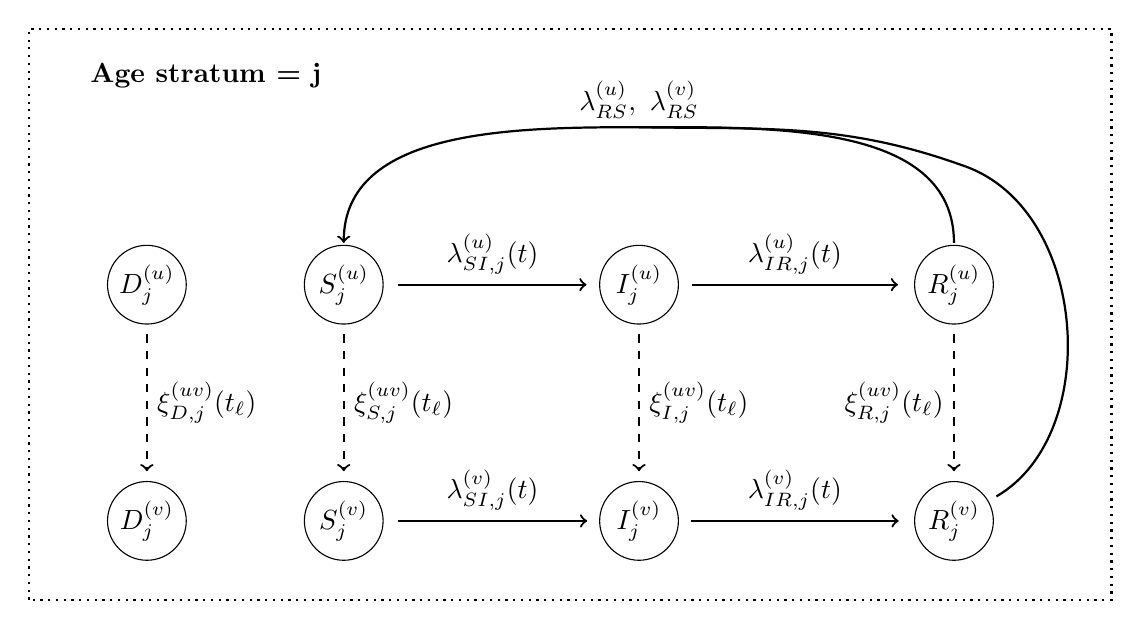
\begin{tikzpicture}
	\draw[thick,dotted] (-2.75,1) rectangle (11,8.25);
	\node at (-0.5,7.25) [label={\textbf{Age stratum = j}}] {};
	\draw (-1.25,5) circle(0.5) node (Dju) {$D_j^{(u)}$};
	\draw (1.25,5) circle(0.5) node (Sju) {$S_j^{(u)}$};
	\draw (5,5) circle(0.5) node (Iju) {$I_j^{(u)}$};
	\draw (9,5) circle(0.5) node (Rju) {$R_j^{(u)}$};
	\draw (-1.25,2) circle(0.5) node (Djv) {$D_j^{(v)}$};
	\draw (1.25,2) circle(0.5) node (Sjv) {$S_j^{(v)}$};
	\draw (5,2) circle(0.5) node (Ijv) {$I_j^{(v)}$};
	\draw (9,2) circle(0.5) node (Rjv) {$R_j^{(v)}$};
	\draw (5,7) coordinate (rec) {};
	\draw (5,7.35) node (reclab) {$ \lambda_{RS}^{(u)},\ \lambda_{RS}^{(v)} $};
	\draw (9.15,6.5) coordinate (rec2) {};
	
	\draw [thick,shorten >=0.25cm,shorten <=0.25cm,->] (Sju) -- (Iju) node[midway,above] {$ \lambda_{SI,j}^{(u)}(t) $};
	\draw [thick,shorten >=0.25cm,shorten <=0.25cm,->] (Iju) -- (Rju) node[midway,above] {$ \lambda_{IR,j}^{(u)}(t) $};
	\draw [thick,shorten >=0.25cm,shorten <=0.25cm,->] (Sjv) -- (Ijv) node[midway,above] {$ \lambda_{SI,j}^{(v)}(t) $};
	\draw [thick,shorten >=0.25cm,shorten <=0.25cm,->] (Ijv) -- (Rjv) node[midway,above] {$ \lambda_{IR,j}^{(v)}(t) $};
	
	\draw [dashed,thick,shorten >=0.25cm,shorten <=0.25cm,->] (Dju) -- (Djv) node[midway,right] {$ \xi_{D,j}^{(uv)}(t_\ell) $};
	\draw [dashed,thick,shorten >=0.25cm,shorten <=0.25cm,->] (Sju) -- (Sjv) node[midway,right] {$ \xi_{S,j}^{(uv)}(t_\ell) $};
	\draw [dashed,thick,shorten >=0.25cm,shorten <=0.25cm,->] (Iju) -- (Ijv) node[midway,right] {$ \xi_{I,j}^{(uv)}(t_\ell) $};
	\draw [dashed,thick,shorten >=0.25cm,shorten <=0.25cm,->] (Rju) -- (Rjv) node[midway,left] {$ \xi_{R,j}^{(uv)}(t_\ell) $};
	
	\draw [thick,shorten >=0cm,shorten <=0.15cm] (Rju) to [out=90, in = 0] (rec);
	\draw [thick,shorten >=0cm,shorten <=0.1cm] (Rjv) to [out=30, in = -20] (rec2);
	\draw [thick] (rec2) to [out=160,in=-1] (rec);
	\draw [thick,shorten >=0.15cm,shorten <=0.0cm,->] (rec) to [out=180, in = 90] (Sju);
	\end{tikzpicture}
	\caption[Diagram of state transitions for an age--vaccination stratified SIRS model for influenza.]{Diagram of state transitions for an age--vaccination stratified SIRS model for influenza in Finland. Both age strata, 0--19 and 20+, have the same compartmental structure. Nodes in circles denote model compartments, which are subscripted with age stratum and superscripted with vaccination status. Solid lines indicate stochastic transitions that occur continuously in time. Rates of disease state transitions, denoted by $ \lambda $, are subscripted with the states from which, and to which, individuals flow and by the age stratum. Superscripts for transition rates indicate vaccination status. Dashed lines represent deterministic forcings from unvaccinated to vaccinated compartments that occur at discrete times. The mass of the forcing at time $ t $, denoted $ \xi(t) $, is subscripted by the compartment and age stratum, and superscripted by the direction of the forcing (unvaccinated to vaccinated).} 
	\label{fig:flu_sirs_diag}
\end{figure}

The contact rate between individuals in age stratum $ j $ and age stratum $ k $, denoted $ C_{jk} $, was based on estimated mean contact rates, appropriately standardized (see Section \ref{sec:flu_contact_rates}), from the Finnish arm of the POLYMOD survey \cite{mossong2008social,polymod} and accessed via the \texttt{socialmixr R} package \cite{funk2018socialmixr}. Sixty percent of contacts in the 0--19 age group were from other individuals age 0--19, while eighty--five percent of the contacts in the 20+ age group were from other adults. The rates, $ \blambda = (\blambda_{Y},\blambda_{A}) $, at which individuals in age--stratum $ j \in \lbrace Y,\ A\rbrace $ transition between disease states are

\begin{equation}\small
\label{eqn:flu_sirs_rates}
\blambda_{j} = \left\lbrace
\begin{array}{ll}
\lambda_{SI,j}^{(u)} = \left [\alpha_{j}(t) + \beta_{j}(t)\left (C_{jk}\left (I_{j}^{(u)} + I_{j}^{(v)}\right ) + (1-C_{jk})\left (I_{k}^{(u)} + I_{k}^{(v)}\right )\right )\right ]S_{j}^{u} \\ 
\lambda_{SI,j}^{(v)} = \nu\left [\alpha_{j}(t) + \beta_{j}(t)\left (C_{jk}\left (I_{j}^{(u)} + I_{j}^{(v)}\right ) + (1-C_{jk})\left (I_{k}^{(u)} + I_{k}^{(v)}\right )\right )\right ]S_{j}^{v}\\
\lambda_{IR,j}^{(u)} = \mu_{j} I_{j}^{(u)} \\
\lambda_{IR,j}^{(v)} = \mu_{j} I_{j}^{(v)} \\
\lambda_{RS,j}^{(u)} = \omega R_{j}^{(u)} \\
\lambda_{RS,j}^{(v)} = \omega R_{j}^{(v)}
\end{array}
\right .
\end{equation}

At weekly intervals, we deterministically force individuals from unvaccinated model compartments to the corresponding vaccinated compartments. Following \cite{shubin2016revealing}, we assume that vaccine doses were distributed proportionally to the number of individuals in each unvaccinated compartment of the corresponding age stratum. In \cite{shubin2016revealing}, it was assumed that vaccination was fully protective with 80\% probability two weeks after administration. Here, we will assume that the vaccine is partially protective in that it reduces the rate at which vaccinated individuals become infected. We do not assume that VE for susceptibility varies by age, and also do not model vaccine efficacy for infectiousness or recovery due to the limited extent of the data. To account for the time required to elicit an immune response, we apply the deterministic forcing at the beginning of week after the time when each dose count was indexed. Suppose that at the end of week $ \ell $ we have $ \bX_j^{(u)}(t_\ell) = \left (S_j^{(u)}(t_\ell),\ I_j^{(u)}(t_\ell),\ R_j^{(u)}(t_\ell),\ D_j^{(u)}(t_\ell)\right ) $ unvaccinated susceptible, infected, recovered, and detached individuals in age stratum $ j $ and $ \bX_j^{(v)}(t_\ell) = \left (S_j^{(v)}(t_\ell),\ I_j^{(v)}(t_\ell),\ R_j^{(v)}(t_\ell),\ D_j^{(v)}(t_\ell\right ) $ vaccinated individuals, and that $ V_j(t_\ell) $ vaccine doses were recorded for stratum $ j $ in that week. We apply the vaccine forcing to the initial state for the following week: 
\begin{align}
\label{eqn:vacc_forcing}
\begin{split}
	\bX_{j}^{(u)}(t_\ell^+) &= \bX_j^{(u)}(t_\ell) - V_j(t_\ell)\frac{\bX_{j}^{(u)}(t_\ell)}{\sum\bX_{j}^{(u)}(t_\ell)}, \\
	\bX_{j}^{(v)}(t_\ell^+) &= \bX_j^{(v)}(t_\ell) + V_j(t_\ell)\frac{\bX_{j}^{(u)}(t_\ell)}{\sum\bX_{j}^{(u)}(t_\ell)}.
\end{split}
\end{align}
Thus, the vaccination forcing affects the initial condition for the period $ (t_\ell,t_{\ell+1}] $, not the state at time $ t_\ell $. 

The diffusion approximation for the MJP is a real--valued process, $ \bX $, that in its infinite population limit evolves as a deterministic system of ODEs. The state space of $ \bX $ is defined in terms of compartment volumes, $ \mcS_X^R $, and with corresponding cumulative incidence process, $ \bN $, with state space $ \mcS_N^R $. Note that the boundary conditions on the state spaces of $ \bX^c $ and $ \bN^c $, and similarly of $ \bX $ and $ \bN $, ensure positivity of compartment counts and monotonicity of cumulative incidence paths, and that the compartment counts each age--vaccination stratum sum to the number of individuals in that stratum, e.g., $ S_{Y}^{(u)}(t) + I_{Y}^{(u)}(t) + R_{Y}^{(u)}(t)+ D_{Y}^{(u)}(t) = N_{Y}^{(u)}(t) $. Due to the complexity of the model, we will rely on the deterministic ODE framework that was explored as a comparitor for the LNA in Chapter \ref{chap:lna_for_sems} to facilitate the computation \ref{chap:lna_for_sems}.  

%As in Chapter \ref{chap:lna_for_sems}, we will use the non--centered parameterization of the restarting LNA of the log--transformed SDE to approximate the time--evolution of $ \bX^c $ and $ \bN^c $. Algorithm \ref{alg:doLNA2} details the procedure for mapping standard normal LNA draws onto an LNA sample path with vaccination forcings.

\subsubsection{Reproduction numbers}
\label{subsubsec:stratmod_repnumbs}
The basic reproduction number, $ R_0 $, and its variants describe the propensity of an outbreak to spread through a population \cite{heffernan2005perspectives,van2008further}. $ R_0 $ is loosely interpreted as the average number of secondary infections arising from a single infected individual in a completely susceptible population. An outbreak will fail to sustain itself (almost surely when it evolves deterministically, but in reality with high probability due to the inherently stochastic nature of epidemics) when $ R_0 < 1 $. For this reason, epidemiologists often quantify the effectiveness of a control measure by estimating the extent to which the intervention reduces $ R_0 $. We can interpret the basic reproduction number as an intrinsic reproduction number when there is an exogenous contribution to force of infection \cite{blackwood2018introduction}. From a modeling perspective, is important to understand not only how $ R_0 $ affects the transmission dynamics, but also how various aspects of the model interact to affect $ R_0 $. 

The basic reproduction number of a structured SEM can be obtained by computing the spectral radius (absolute value of the dominant eigenvalue) of the next generation matrix (NGM) for the linearized system of ODEs specifying the flow in and out of states at infection \cite{heffernan2005perspectives,van2017reproduction,van2008further}. The $ i,j $ element of the NGM gives the expected number of secondary infections in age stratum $ i $ given an index infection in stratum $ j $. Noting that vaccinated and unvaccinated invididuals in this model are equally transmissive and have the same mean infectious period durations, we obtain the age--structured next generation matrix
\begin{align}
\label{eqn:sirs_ngm_full}
\bK &= 
	\left (
	\begin{array}{cc}
	K_{YY} & K_{YA} \\
	K_{AY} & K_{AA}
	\end{array}
	\right ) =\left (
	\begin{array}{cc}
	\frac{C_{YY}\beta_Y\left (N_Y^{(u)} + \nu_YN_Y^{(v)}\right )}{\mu_Y} & \frac{C_{YA}\beta_Y\left (N_Y^{(u)} + \nu_YN_Y^{(v)}\right )}{\mu_A} \\[2ex]
	\frac{C_{AY}\beta_A\left (N_A^{(u)} + \nu_AN_A^{(v)}\right )}{\mu_Y} & \frac{C_{AA}\beta_A\left (N_A^{(u)} + \nu_AN_A^{(v)}\right )}{\mu_A}
	\end{array}
	\right ).
\end{align}
The basic reproduction number is 
\begin{align}
\label{eqn:sirs_R0}
R_0 = \frac{1}{2}\left (K_{YY} + K_{AA}\right ) + \frac{1}{2}\sqrt{(K_{YY} - K_{AA})^2 + 4K_{YA}K_{AY}}.
\end{align}

Note that is possible for the outbreak to persist, i.e., $ R_0 > 1 $,  when the intrinsic reproduction number in one of the strata is below 1, e.g., $ K_{YY} <1$, even though most transmission arises from within--group contacts. However, $ R_0 <$ will be less than 1 if both $ K_{YY} <1 $ and $ K_{AA} <1 $.

Furthermore, the basic reproduction number is greater than the average of intrinsic reproduction numbers, $ K_{YY} $ and $ K_{AA} $, since the second term on the right hand side of (\ref{eqn:sirs_R0}) will typically be positive. Similarly, the variance of $ R_0 $ is also greater than the average of variances of $ K_{YY} $ and $ K_{AA} $. For these reasons, we should consider how $ K_{YY} $ and $ K_{AA} $ interact to induce a prior over $ R_0 $ when parameterizing the model. Note that if the cross--stratum contact rates were negligible, $ R_0 $ would behave like the average of intrinsic reproduction numbers plus a term proportional to the absolute difference between $ K_{YY} $ and $ K_{AA} $. This suggests that prior information about the intrinsic reproduction numbers, either individually (our preference) or about their average and difference, could help identify $ R_0 $. We should also keep in mind that our model is more complicated since the cross stratum terms are not negligible ($ C_{AA} = 0.6 $, $ C_{YY}=0.85 $), hence
\begin{align*}
K_{YA} &= \frac{(1 - C_{YY})}{C_{YY}}\frac{\mu_Y}{\mu_A}K_{YY},\hspace{0.25in}
K_{AY} = \frac{(1 - C_{AA})}{C_{AA}}\frac{\mu_A}{\mu_Y}K_{AA},\\
&\implies K_{YA}K_{AY} = \frac{(1 - C_{YY})(1-C_{AA})}{C_{YY}C_{AA}}K_{YY}K_{AA}.
\end{align*} 
Thus, $ R_0 $ is the average of $ K_{YY} $ and $ K_{AA} $, plus a non--linear function of $ K_{YY} $ and $ K_{AA} $.

Finally we emphasize the importance of accounting for all of the parameters that contribute the intrinsic reproduction numbers, and by extension $ R_0 $, when specifying priors and parameterizing the estimation scale of the MCMC. In particular, it is critical to note that the effective population size might be lower than the nominal population size because of vaccination and depletion of susceptibles. We can easily misspecify the scales of prior distributions for the reproduction numbers, or select an inefficient parameterization for the MCMC estimation scale, by neglecting this dynamic. In our model, for example, the value of $ R_0 $ in the first season, and the rate at which recovered individuals lose immunity, will affect the effective population size at the beginning of the second season. 

\subsection{Flexible Models for the Force of Infection with Gaussian Markov Random Fields}
\label{subsec:flu_gmrf}

We will model the time--varying force of infection using first order GMRFs for the log intrinsic reproduction numbers and the effective rate of exogenous infectious contacts in each age stratum. The GMRFs are separately specified over three epochs corresponding to the period one month before the first detected case until the start of the Finnish school year in 2009, the beginning of the Finnish school year in 2009 until its start in 2010 (including the inter--season period), and the second epidemic season beginning at the start of the Finnish school year, 2010. These epochs correspond to epiweeks 15, 2009 through epiweek 34, 2009, epiweek 35, 2009 through epiweek 32, 2010, and epiweek 33, 2010 through epiweek 22, 2011. We will assume that the intrinsic reproduction numbers are homogeneous over the inter--season period, from epiweek 16, 2010 -- epiweek 32, 2010.

Let $ \bpsi_{j} = \lbrace\psi_{j,\ell}:\ \ell \in 0,\dots,52,71,\dots,112\rbrace $ be the vector of intrinsic reproduction numbers for stratum $ j \in \lbrace Y,A \rbrace$, ignoring the relative contact rates, $ C_{jk} $, and vaccination. The reproduction number in time interval $ \ell $, indexed in weeks from epiweek 15, 2009, is
\begin{equation}
\label{eqn:R0t_novacc}
\psi_{j,\ell} = \frac{\beta_j(t_\ell)N_js_j}{\mu_j},
\end{equation}
where $ \beta_j(t_\ell) $ is the per--contact infection rate, $ \mu_j $ is the recovery rate, $ N_j $ is the size of the age stratum, and $ s_j $ is the fraction of individuals in stratum $ j $ that are susceptible.
 
When transmission is sustained at near--endemic levels, we should expect that the effective reproduction numbers are near one, or perhaps slightly above. Let $ \nu $ be the relative rate of infectious contact among vaccinated individuals, i.e., one minus the vaccine efficacy for susceptibility. The effective reproduction number, which accounts for the effects of vaccination and depletion of susceptibles, is 
\begin{equation}
\label{eqn:Reff_t}
\psi_{j,\ell}^{eff} = \frac{\beta_j(t_\ell)_j\left (S^{(u)}_j(t_\ell) + S^{(v)}_j(t_\ell)\nu\right )}{\mu_j}
\end{equation}
If vaccination does not increase the rate of infectious contact (and we will assume it does not), then $ \psi_{j,\ell}^{eff} < \psi_{j,\ell} $ since $ \nu\in[0,1] $ and $ (S^{(u)}_j(t_\ell) + S^{(v)}_j(t_\ell) < N_js_j $. It is critical to account for this when specifying priors for the basic intrinsic reproduction numbers at the start of each epoch. It would not do, for instance, to set priors for the intrinsic basic reproduction numbers at the beginning of the third epoch that nominally concentrate mass near one since this would imply that the effective reproduction numbers are far below one due to vaccination and depletion of susceptibles during the first wave of the outbreak. Our approach will be to assign priors to the vaccination adjusted intrinsic reproduction numbers at the beginning of each epoch, $ \psi_{j,\ell}^\prime = \psi_{j,\ell}  \left (1 - P^v_j(t_\ell) + P^v_j(t_\ell)\right ) $, where $ P_j^v(t_\ell) $ is the vaccination coverage in stratum $ j $ at $ t_\ell $. 

We denote by $ \Delta $ the first--order forward difference operator, i.e., $ \Delta X_j = X_{j+1} - X_j $. The first--order differences of the log intrinsic reproduction numbers for stratum $ j $ in each epoch are assigned a Gaussian prior with mean zero and variance $ \sigma^2_{j,\ell} $. The sub--model for intrinsic reproduction numbers in stratum $ j $ is

\begin{small}
	\begin{align}
	\log(\psi_{j,\ell}) &\sim \mcN(\mu_{j,\ell},\tau_{j,\ell}^2),&\ &\ell= 0,19,71, \nonumber\\
	\log(\sigma_{j,\ell}) &\sim \mcN(m_{j,\ell}, s_{j,\ell}^2),&\ &\ell=0,19,71, \nonumber\\
	\Delta\log(\psi_{j,\ell})&\sim \mcN(0, \sigma^2_{j,0}),&\ &\ell=0,\dots,17, \nonumber\\
	\Delta\log(\psi_{j,\ell})&\sim \mcN(0, \sigma^2_{j,19}),&\ &\ell=19,\dots,51, \nonumber\\
	\Delta\log(\psi_{j,\ell})&\sim \mcN(0, \sigma^2_{j,71}),&\ &\ell=71,\dots,111, \nonumber\\
	\log(\psi_{j,\ell}) &= \log(\psi_{j,0}) + \sum_{k=0}^{\ell-1}\Delta\log(\psi_{j,k}),&\ &\ell = 1,\dots,17, \nonumber\\
	\log(\psi_{j,\ell}) &= \log(\psi_{j,19}) + \sum_{k=0}^{\ell-1}\Delta\log(\psi_{j,19+k}),&\ &\ell = 19,\dots,52, \nonumber\\
	\log(\psi_{j,\ell}) &= \log(\psi_{j,71}) + \sum_{k=0}^{\ell-1}\Delta\log(\psi_{j,71+k}),&\ &\ell = 72,\dots,112. \nonumber \\
	\beta_j(t_\ell) &= \psi_{j,\ell}N_j/\left (\mu_{j}(t_\ell)(1 - P^v_j(t_\ell) + P_j^v(t_\ell)\nu_j)\right ),&\ &\ell=0,\dots,52,71,\dots,112. \nonumber
	\end{align}
\end{small}

The induced GMRF prior for the vaccination adjusted basic reproduction numbers is given in Figure \ref{fig:flurw1prior}. 

In practice, we will use the following partially non--centered parameterization:
\begin{small}
	\begin{align}
	\log(\psi_{j,\ell}) &\sim \mcN(\mu_{j,\ell},\tau_{j,\ell}^2),&\ &\ell= 0,19,71, \nonumber\\
	Z_{\log(\sigma_{j,\ell})} &\sim \mcN(0,1),&\ &\ell=0,19,71, \nonumber \\
	Z_{\Delta\log(\psi_{j,\ell})} &\sim \mcN(0,1),&\ &\ell=0,\dots,17,19,\dots,51,71,\dots,111, \nonumber \\ 
	\log(\sigma_{j,\ell}) &= m_{j,\ell} + s_{j,\ell}Z_{\log(\sigma_{j,\ell})},&\ &\ell = 0,19,71,\nonumber\\
	\Delta\log(\psi_{j,\ell})&= \sigma_{j,0} Z_{\Delta\log(\psi_{j,\ell})},&\ &\ell=0,\dots,17, \nonumber\\
	\Delta\log(\psi_{j,\ell})&= \sigma_{j,19} Z_{\Delta\log(\psi_{j,\ell})},&\ &\ell=19,\dots,51, \nonumber\\
	\Delta\log(\psi_{j,\ell})&= \sigma_{j,71} Z_{\Delta\log(\psi_{j,\ell})},&\ &\ell=71,\dots,111, \nonumber\\
	\log(\psi_{j,\ell}) &= \log(\psi_{j,0}) + \sum_{k=0}^{\ell-1}\Delta\log(\psi_{j,k}),&\ &\ell = 1,\dots,17, \nonumber\\
	\log(\psi_{j,\ell}) &= \log(\psi_{j,19}) + \sum_{k=0}^{\ell-1}\Delta\log(\psi_{j,19+k}),&\ &\ell = 19,\dots,52, \nonumber\\
	\log(\psi_{j,\ell}) &= \log(\psi_{j,71}) + \sum_{k=0}^{\ell-1}\Delta\log(\psi_{j,71+k}),&\ &\ell = 72,\dots,112. \nonumber \\
	\beta_j(t_\ell) &= \psi_{j,\ell}N_j/\left (\mu_{j}(t_\ell)(1 - P^v_j(t_\ell) + P_j^v(t_\ell)\nu_j)\right ),&\ &\ell=0,\dots,52,71,\dots,112. \nonumber
	\end{align}
\end{small}

We similarly assign a first order GMRF prior to the effective number of exogenous infectious contacts for each age stratum. Note that this term is somewhat of a catch--all for infectious contacts that arise outside of the density dependent mixing of susceptible and infected individuals. The rate of exogenous infection may be loosely interpreted as either the baseline rate of infectious contact or as the rate of infection from outside the population. Let $ \alpha^\prime_{j,\ell} = \alpha_{j,\ell}N_js_j $ denote the rate of exogenous infection for age stratum $ j $ in week $ \ell $, scaled by the effective stratum size. The GMRF prior for $ \balpha^\prime_j = \lbrace\alpha^\prime_{j,\ell}:\ \ell=0,\dots,52,71,\dots,112\rbrace $ is
\begin{small}
	\begin{align}
	\log(\alpha^\prime_{j,\ell}) &\sim \mcN(\mu_{j,\ell},\tau_{j,\ell}^2),&\ &\ell= 0,19,71, \nonumber\\
	\log(\sigma_{j,\ell}) &\sim \mcN(m_{j,\ell}, s_{j,\ell}^2),&\ &\ell=0,19,71, \nonumber\\
	\Delta\log(\alpha^\prime_{j,\ell})&\sim \mcN(0, \sigma^2_{j,0}),&\ &\ell=0,\dots,17, \nonumber\\
	\Delta\log(\alpha^\prime_{j,\ell})&\sim \mcN(0, \sigma^2_{j,19}),&\ &\ell=19,\dots,51, \nonumber\\
	\Delta\log(\alpha^\prime_{j,\ell})&\sim \mcN(0, \sigma^2_{j,71}),&\ &\ell=71,\dots,111, \nonumber\\
	\log(\alpha^\prime_{j,\ell}) &= \log(\alpha^\prime_{j,0}) + \sum_{k=0}^{\ell-1}\Delta\log(\alpha^\prime_{j,k}),&\ &\ell = 1,\dots,17, \nonumber\\
	\log(\alpha^\prime_{j,\ell}) &= \log(\alpha^\prime_{j,19}) + \sum_{k=0}^{\ell-1}\Delta\log(\alpha^\prime_{j,19+k}),&\ &\ell = 19,\dots,52, \nonumber\\
	\log(\alpha^\prime_{j,\ell}) &= \log(\alpha^\prime_{j,71}) + \sum_{k=0}^{\ell-1}\Delta\log(\alpha^\prime_{j,71+k}),&\ &\ell = 72,\dots,112. \nonumber \\
	\alpha_{j,\ell} &= \alpha^\prime_{j,\ell}/N,&\ &\ell=0,\dots,52,71,\dots,112. \nonumber
	\end{align}
\end{small}

Again, we will use a partially non--centered parameterization in practice.
\begin{small}
	\begin{align}
	\log(\alpha^\prime_{j,\ell}) &\sim \mcN(\mu_{j,\ell},\tau_{j,\ell}^2),&\ &\ell= 0,19,71, \nonumber\\
	Z_{\log(\sigma_{j,\ell})} &\sim \mcN(0,1),&\ &\ell=0,19,71, \nonumber \\
	Z_{\Delta\log(\alpha^\prime_{j,\ell})} &\sim \mcN(0,1),&\ &\ell=0,\dots,17,19,\dots,51,71,\dots,111, \nonumber \\ 
	\log(\sigma_{j,\ell}) &= m_{j,\ell} + s_{j,\ell}Z_{\log(\sigma_{j,\ell})},&\ &\ell = 0,19,71,\nonumber\\
	\Delta\log(\alpha^\prime_{j,\ell})&= \sigma_{j,0} Z_{\Delta\log(\alpha^\prime_{j,\ell})},&\ &\ell=0,\dots,17, \nonumber\\
	\Delta\log(\alpha^\prime_{j,\ell})&= \sigma_{j,19} Z_{\Delta\log(\alpha^\prime_{j,\ell})},&\ &\ell=19,\dots,51, \nonumber\\
	\Delta\log(\alpha^\prime_{j,\ell})&= \sigma_{j,71} Z_{\Delta\log(\alpha^\prime_{j,\ell})},&\ &\ell=71,\dots,111, \nonumber\\
	\log(\alpha^\prime_{j,\ell}) &= \log(\alpha^\prime_{j,0}) + \sum_{k=0}^{\ell-1}\Delta\log(\alpha^\prime_{j,k}),&\ &\ell = 1,\dots,17, \nonumber\\
	\log(\alpha^\prime_{j,\ell}) &= \log(\alpha^\prime_{j,19}) + \sum_{k=0}^{\ell-1}\Delta\log(\alpha^\prime_{j,19+k}),&\ &\ell = 19,\dots,52, \nonumber\\
	\log(\alpha^\prime_{j,\ell}) &= \log(\alpha^\prime_{j,71}) + \sum_{k=0}^{\ell-1}\Delta\log(\alpha^\prime_{j,71+k}),&\ &\ell = 72,\dots,112. \nonumber \\
	\alpha_{j,\ell} &= \alpha^\prime_{j,\ell}/N,&\ &\ell=0,\dots,52,71,\dots,112 \nonumber
	\end{align}
\end{small}

The initial reproduction numbers, for which we retain the centered parameterization, are blocked with other model parameters and updated using a multivariate normal slice sampler (MVNSS). The non--centered GMRF differences and their standard deviations are updated 
%jointly with the LNA path 
using elliptical slice sampling (Algorithm \ref{alg:elliptical_slice_sampler}).
%(Algorithm \ref{alg:elliptss_lna_gmrf}). 
Readers familiar with GMRFs will note the, somewhat unconventional, Gaussian prior for the standard deviation of the GMRF increments. This choice was made for computational reasons in order to facilitate joint updates of the GMRF and its hyper--parameters. Alternating between field and hyper--parameter updates is known to results in poorly mixing MCMC chains as large updates to the hyper--parameters quickly result in fields that are not concordant with the data  \cite{knorr2002block,murray2010hyper}. 

\subsection{Sampling from the Posterior}
\label{subsec:flu_mcmc}

Let $ \bZ = \left (\bZ^F,\bZ^{\btheta_F}\right ) $ denote the vector of i.i.d. standard normal draws for the GMRF increments and GMRF hyperparameters, $ \doGMRF(\bZ;\btheta) $ be the operation for computing the GMRF from its draws and hyperparameters, and $ \pi(\btheta) $ be the prior distributions for the other model parameters. Let $ \mathcal{T} = \lbrace t_\ell:\ \ell = 1,\dots,52,71,\dots,113 \rbrace $ denote the set of observation times. Our MCMC will target the posterior
\begin{align}
\label{eqn:flu_posterior}
\pi(\btheta,\bZ | \bY) &\propto \pi(\bZ)\pi(\btheta)\pi(\bY|\btheta,\bZ) \nonumber\\
&= \pi(\bZ)\pi(\btheta) \prod_{t_\ell\in\mathcal{T}}\prod_{j\in\lbrace Y,A\rbrace} \Pr\left (Y_{j}(t_\ell) | \doGMRF(\bZ),\btheta,\mcI)\right )
\end{align}
MCMC proceeds by alternately updating $ \bZ|\bY,\btheta $ using ElliptSS (Algorithm \ref{alg:elliptss_lna_gmrf}) and MVNSS updates for $ \btheta|\bY,\bZ $ (Algorithm \ref{alg:mvnss}). Priors for model parameters were informative are detailed in Section \ref{subsec:flu_priors} and additional MCMC details are provided in Section \ref{subsec:flu_mcmc_details}. Generally speaking, priors for parameters were informative and we made an effort to choose priors that were based on published estimates from other studies.

%Let $ \bZ = \left (\bZ^X,\bZ^F,\bZ^{\btheta_F}\right ) $ denote the vector of i.i.d. standard normal draws for the LNA, GMRF increments, and GMRF hyperparameters, and let $ \pi(\btheta) $ be the prior distributions for the other model parameters. Let $ \mathcal{T} = \lbrace t_\ell:\ \ell = 1,\dots,52,71,\dots,113 \rbrace $ denote the set of observation times. Our MCMC will target the posterior
%\begin{align}
%\label{eqn:flu_posterior}
%\pi(\btheta,\bZ | \bY) &\propto \pi(\bZ)\pi(\btheta)\pi(\bY|\btheta,\bZ) \nonumber\\
%&= \pi(\bZ)\pi(\btheta) \prod_{t_\ell\in\mathcal{T}}\prod_{j\in\lbrace Y,A\rbrace} \Pr\left (Y_{j}(t_\ell) | \doLNA2(\bZ,\btheta,\mcI,\bxi)\right )
%\end{align}
%MCMC proceeds by alternately updating $ \bZ|\bY,\btheta $ using ElliptSS (Algorithm \ref{alg:elliptss_lna_gmrf}) and MVNSS updates for $ \btheta|\bY,\bZ $ (Algorithm \ref{alg:mvnss}). 

\section{Results}
\label{sec:flu_results}

\subsection{Incidence}
\label{subsec:flu_incid_res}
Estimates of cumulative incidence and attack rates by season and age group are reported in Table \ref{tab:flu_attack_rates}. We estimate that there were approximately 532,000 (95\% BCI: 393,000, 703,000) infections in the first epidemic season, and an additional 240,000 (95\% BCI: 172,000, 333,000) cases during the second season. These estimates would correspond to estimated attack rates of 7.4\%--13.1\% during the first season, and 3.2\%--6.2\% in the second season if each individual was infected only once. The estimated attack rates were substantially higher among youths than adults in the first epidemic season, and slightly higher during the second season. The estimated incidence over the inter--season period was low; 110 cases (95\% BCI: 50, 250) among youths, and 330 cases (95\% BCI: 150, 710) among adults. 

\begin{sidewaystable}[htbp]
	\caption{Estimated infections (thousands) and attack rates by season and age stratum. Attack rates are calculated as the number of infections divided by the size of each stratum, assuming that cases are unique.}
	\label{tab:flu_attack_rates}
	\centering\footnotesize
	\begin{tabular}{lrrrrrr}
		\hline
		&\multicolumn{6}{c}{\textbf{Time varying dynamics}}\\
		\cmidrule{2-7} & \multicolumn{2}{c}{\textit{Season 1}} & \multicolumn{2}{c}{\textit{Season 2}} & \multicolumn{2}{c}{\textit{Both Seasons}}\\
		\cmidrule(r){2-3}\cmidrule(lr){4-5}\cmidrule(l){6-7} & 
		Incidence & Attack rate & Incidence & Attack rate & Incidence & Attack rate \\
		\hline
	Ages 0-19 & 174 (127, 231) & 14.2 (10.4, 18.9) & 68.6 (46.6, 100) & 5.6 (3.8, 8.2) & 244 (181, 321) & 19.9 (14.8, 26.2)\\
	Ages 20+ & 356 (243, 501) & 8.6 (5.9, 12.1) & 171 (117, 245) & 4.1 (2.8, 5.9) & 530 (378, 720) & 12.8 (9.2, 17.4)\\
	All ages & 532 (393, 703) & 9.9 (7.4, 13.1) & 240 (172, 333) & 4.5 (3.2, 6.2) & 774 (586, 1,010) & 14.5 (11, 18.8)\\
		\hline &&&&&&\\
		&\multicolumn{6}{c}{\textbf{Piecewise homogeneous dynamics}}\\
		\cmidrule{2-7}	& \multicolumn{2}{c}{\textit{Season 1}} & \multicolumn{2}{c}{\textit{Season 2}} & \multicolumn{2}{c}{\textit{Both Seasons}}\\
	\cmidrule(r){2-3}\cmidrule(lr){4-5}\cmidrule(l){6-7} & 
	Incidence & Attack rate & Incidence & Attack rate & Incidence & Attack rate \\
	\hline
	Ages\_0-19 & 150 (107, 203) & 12.3 (8.7, 16.6) & 55.1 (34.4, 82) & 4.5 (2.8, 6.7) & 206 (154, 267) & 16.8 (12.6, 21.9)\\
	\hline
	Ages\_20+ & 263 (182, 375) & 6.4 (4.4, 9.1) & 181 (128, 242) & 4.4 (3.1, 5.9) & 445 (324, 598) & 10.8 (7.9, 14.5)\\
	\hline
	All\_ages & 414 (305, 556) & 7.7 (5.7, 10.4) & 236 (178, 309) & 4.4 (3.3, 5.8) & 653 (499, 840) & 12.2 (9.3, 15.7)\\
		\hline
	\end{tabular}
\end{sidewaystable}

\subsection{Transmission Dynamics}
\label{flu_res_dynamics}
Estimates of time varying reproduction numbers and exogenous infections are shown in Figure \ref{fig:flurwodetimevaryingplots} and estimates of model parameters are given in Table \ref{tab:flu_param_ests}. The period just prior to the first detected cases until the start of the Finnish school year in 2009 was characterized by low basic and effective reproduction numbers. The basic reproduction numbers over this period remained at near--endemic levels (95\% BCI: 0.99, 1.00; second and third rows of Figure \ref{fig:flurwodetimevaryingplots}). 

The basic reproduction numbers from the start of the Finnish school year through the peak of the first wave of the outbreak were somewhat higher at around 1.2 (95\% BCI: 1.1, 1.3), increased slightly as the epidemic peaked, but declined below one in early December, 2009, as a result in vaccination. Incidence began to decline, starting in mid--November, preceding the drop in basic reproduction numbers due to vaccination by several weeks, and well before vaccine coverage had reached meaningful levels. The effective reproduction numbers declined throughout the first wave, indicating that the slight increases in rates of infectious contact overwhelmed by depletion of susceptibles.

The vaccination--adjusted basic reproduction numbers at the start of the second season, roughly 1.4 (95\% BCI: 1.3, 1.6), were nominally higher than at the start of the first season. However, these estimates do not account for depletion of susceptibles in the first wave of the outbreak. Effective reproduction numbers at the beginning of second epidemic wave were roughly 1.16 (95\% BCI: 1.10, 1.23), were comparable to effective reproduction numbers during the first wave. Without adjusting for vaccination, the basic reproduction numbers would be in the range of 2.4--4, which is similar to results in \cite{shubin2016revealing}. Accounting for vaccination and depletion of susceptibles brings the adjusted reproduction numbers into the range that is more similar to previous estimates for A(H1N1)pdm09 outbreaks \cite{biggerstaff2014estimates}. 

Figure \ref{fig:flurwodetimevaryingplots} presents the effective and vaccine adjusted type reproduction numbers for the 0--19 and 20+ age strata, which are interpreted as the expected number of secondary cases of any age caused by a single index case in a given age stratum. The type reproduction numbers are the column sums of the basic (vaccine adjusted) and effective NGMs. Note that this definition differs from the definition of type reproduction number in \cite{heesterbeek2007type}, which is the expected number of secondary cases of a particular type given an index case of that type. At the beginning of the first epidemic wave (epiweek 34, 2009), an index youth case was estimated to result in 1.3 (95\% BCI: 1.0, 1.6) secondary cases, while an index adult would result in 1.15 (95\% BCI: 1.0, 1.3) secondary cases. The contribution of youths to the FOI declined dramatically in the second season, while the contribution of adults was roughly the same. At the start of the second season, an index youth case was estimated to lead to 1.0 (95\% BCI: 0.8, 1.25) secondary cases, while an index adult case to 1.2 (1.0, 1.3) secondary cases. The change in the role contribution of youths in the second season can be attributed to the depletion of susceptible youths in the first season due to vaccination and high attack rates in that season. The effective type reproduction numbers in both age strata decline throughout the first wave, while in the second season they increase slightly before again declining as susceptibles deplete. The slight uptick in effective type reproduction numbers at the end of the second season is attributable to loss of immunity among previously infected individuals.  

\begin{sidewaysfigure}[htbp]
	\centering
	\includegraphics[width=0.95\linewidth]{figures/flu_rw_ode_timevarying_plots}
	\caption{Posterior estimates of time varying quantities under time varying dynamics. Estimated incidence (top row), effective reproduction numbers (second row), vaccination adjusted basic reproduction numbers (third row), and exogenous infections (bottom row). $ N_{SI}^j(t), $ is the weekly incidence in age stratum $ j $, $ R_{eff}(t) $ and $ R_{adj}(t) $ are the effective and vaccination--adjusted basic reproduction numbers, $ T_{eff}^j(t) $ is the type reproduction number for stratum $ j $ (expected \# of secondary infections in all strata for a single infected in stratum $ j $), and $ \alpha_j(t) $ is the rate of exogenous infectious contacts for stratum $ j $.}
	\label{fig:flurwodetimevaryingplots}
\end{sidewaysfigure}

The mean infectious period of youths was substantially longer that of adults, 6.5 days (95\% BCI: 4.3 days, 8.8 days) compared with 2.6 days (1.9 days, 3.4 days), respectively. Published point estimates of the serial interval for A(H1N1)pdm09, which is the average time between an index case and a secondary case, and which we might expect to be a bit shorter than the mean infectious period, have mostly been in the 2--3.5 day range \cite{vink2014serial}. Immunity following infection was relatively long--lasting, although a sizable percentage of individuals who were infected lost immunity; 8.2\% (95\% BCI: 3.8\%, 16.2\%) of individuals who had become infected before the start of the second season had lost protection by the beginning of the second season, while the percentage of infected individuals who became infected over both seasons and lost immunity by the end of season two was 10.6\% (95\% BCI: 5.0\%, 19.9\%). The vaccine was estimated to be quite effective,  reducing the rate of infectious contact by 95\% (95\% BCI: 83\%, 99\%). 

\begin{sidewaystable}[htbp]
	\caption[Posterior estimates of SIRS model parameters for pandemic A(H1N1) influenza in Finland.]{Posterior estimates of SIRS model parameters for pandemic A(H1N1) influenza in Finland. Intrinsic reproduction numbers account for vaccine coverage and vaccine efficacy via (\ref{eqn:R0t_vacc}).} 
	\label{tab:flu_param_ests}
	\centering\footnotesize
	\begin{tabular}{clrr}
		\hline
		&&\multicolumn{2}{c}{\textbf{Dynamics}}\\
		\cmidrule{3-4}\textbf{Parameter} & \textbf{Interpretation} & \textit{Time varying} & \textit{Piecewise homogeneous}\\
		\hline
		$ \psi_{Y,0} $ & Intrinsic $ R_0 $ for youths at epiweek 15, 2009  & 1.1 (1.0, 1.2) & 1.1 (1.0, 1.2)\\
		$ \psi_{Y,18} $ & Intrinsic $ R_0 $ for youths at epiweek 34, 2009 & 1.5 (1.1, 1.8) & 1.6 (1.3, 1.9)\\
		$ \psi_{Y,71} $ & Intrinsic $ R_0 $ for youths at epiweek 33, 2010 & 1.2 (0.93, 1.5) & 1.2 (0.94, 1.5)\\
		$ \psi_{A,0} $ & Intrinsic $ R_0 $ for adults at epiweek 15, 2009  & 1.1 (1, 1.2) & 1.1 (1, 1.1)\\
		$ \psi_{A,18} $ & Intrinsic $ R_0 $ for adults at epiweek 34, 2009 & 1.1 (0.95, 1.2) & 1.1 (0.96, 1.2)\\
		$ \psi_{A,71} $ & Intrinsic $ R_0 $ for adults at epiweek 33, 2010 & 1.4 (1.1, 1.8) & 1.6 (1.4, 1.8)\\
		$ 1/\mu_{Y} $ & Mean infectious period for youths (days) & 6.5 (4.3, 8.8) & 7.5 (5.5, 9.5)\\
		$ 1/\mu_A $ & Mean infectious period for adults (days) & 2.6 (1.9, 3.4) & 2.9 (2.2, 3.8)\\
		$ 1/\mu $ & Mean duration of immunity (years) & 9.3 (4.5, 21) & 9.9 (4.8, 21)\\
		$ \nu $ & 1 - VE for susceptibility & 0.05 (0.01, 0.17) & 0.04 (0.01, 0.13)\\
		$ \rho_Y $ & Mean case detection rate for youths & 0.008 (0.006, 0.012) & 0.008 (0.006, 0.011)\\
		$ \rho_A $ & Mean case detection rate for adults & 0.003 (0.002, 0.005) & 0.003 (0.002, 0.004)\\		
		$ 1/\sqrt{\phi_Y} $ & Negative binomial overdispersion for youths & 0.99 (0.82, 1.2) & 1 (0.85, 1.3)\\
		$ 1/\sqrt{\phi_A} $ & Negative binomial overdispersion for adults & 0.97 (0.83, 1.2) & 1 (0.83, 1.2)\\
		\hline
	\end{tabular}
\end{sidewaystable}

The posterior predictive distributions for cases (Figure \ref{fig:flupostpredsrwode}) suggests that the model does a better job reconstructing the second epidemic season than the first, particularly among individuals ages 0--19. The model seems to substantially underestimate the peak of the outbreak in the first season. This might seem somewhat surprising given that the attack rates in the first season were quite high. One possibility is that heterogeneity in detection rates is confounding our estimates of the unobserved epidemic process. In their analysis of this data, \cite{shubin2016revealing} estimated that detection was positively associated with incidence. It is also possible that misspecification of the effective population size could be contributing to the lack of model fit. This might occur, for example, if a meaningful percentage of the population were geographically separated from the areas with intense transmission, or were immune due to exposure to A(H1N1) early in life (as might be the case for older individuals who had antibodies from the 1918 pandemic).  

\begin{figure}[htbp]
	\centering
	\includegraphics[width=\linewidth]{figures/flu_postpreds_rw_ode}
	\caption{Posterior predictive distributions of a stratified SIRS ODE model with time varying dynamics for A(H1N1)pdm09 in Finland.}
	\label{fig:flupostpredsrwode}
\end{figure}


\subsection{Piecewise Homogeneous Dynamics}
\label{subsec:flu_res_homog}

For comparison, we fit a model where the outbreak dynamics were piecewise homogeneous (PH) in each epoch. The vaccination adjusted basic reproduction number was estimated for each of the three epochs, and the per--contact infection rate computed from the vaccination adjusted basic reproduction number. The rate of exogenous infection was also constant within each epoch, but no other aspects of the model dynamics differed from the previous model. Posterior distributions of time varying quantities are presented in Figure \ref{fig:fluconstodetimevaryingplots}, and posterior estimates of model parameters are summarized in Table \ref{tab:flu_param_ests}. 

\begin{sidewaysfigure}[htbp]
	\centering
	\includegraphics[width=0.95\linewidth]{figures/flu_const_ode_timevarying_plots}
	\caption{Posterior estimates of time varying quantities under piecewise homogeneous dynamics. Estimated incidence (top row), effective reproduction numbers (second row), vaccination adjusted basic reproduction numbers (third row), and exogenous infections (bottom row). $ N_{SI}^j(t), $ is the weekly incidence in age stratum $ j $, $ R_{eff}(t) $ and $ R_{adj}(t) $ are the effective and vaccination--adjusted basic reproduction numbers, $ T_{eff}^j(t) $ is the type reproduction number for stratum $ j $ (expected \# of secondary infections in all strata for a single infected in stratum $ j $), and $ \alpha_j(t) $ is the rate of exogenous infectious contacts for stratum $ j $.}
	\label{fig:fluconstodetimevaryingplots}
\end{sidewaysfigure}


The GMRF and PH models are qualitatively quite similar. Estimated attack rates were comparable, though perhaps slightly higher under the PH model. Estimates of the parameters that govern the model dynamics were also largely in agreement, with dwell times in the infectious and recovered states being slightly longer under the PH model. The rate of exogeneous infections among adults was higher under the PH model in the first epoch, but otherwise comparable. The posterior predictive performance of the PH model is nearly identical to that of the GMRF model (Figure \ref{fig:flu_rw_const_ppicomp}), though PPIs under the PH model tended to be slightly wider. 

On the whole, the similarity between the PH and GMRF models is unsurprising given that the variability of the GMRF was fairly constrained and that we used fairly informative priors. However, it is also possible that the introduction of two changepoints in the PH model were sufficient to capture the largest changes in the outbreak dynamics and that within--season heterogeneity in the dynamics was minor. For comparison, we fit a supplementary PH model with only two epochs so that the dynamics were homogeneous over the entire first year. When we omit the changepoint at the start of the Finnish school year, 2009, the model estimates virtually no decline in attack rates for the second season (Figure \ref{fig:fluincid2epochode}). Inspection of the posterior predictive distributions for the two epoch PH model (Figure \ref{fig:flupostpred2epochode}) reveals much more severe misspecification in the sub--models for both age groups during the first epidemic season.  

\begin{figure}[htbp]
	\centering
	\includegraphics[width=0.9\linewidth]{figures/flu_postpreds_const_ode}
	\caption{Posterior predictive distributions of a stratified SIRS ODE model with piecewise homogeneous dynamics over three epochs for A(H1N1)pdm09 in Finland.}
	\label{fig:flupostpredsconstode}
\end{figure}

\begin{figure}[htbp]
	\centering
	\includegraphics[width=0.9\linewidth]{figures/flu_rw_const_ppicomp}
	\caption[Comparison with posterior predictive p-values and relative predictive interval widths for SIRS models with time varying and piecewise homogeneous dynamics.]{Comparison of models with time--varying (GMRF) and piecewise homogeneous (PH) force of infection using posterior predictive p-values (PPPs) and relative posterior predictive interval (PPI) widths. Each point corresponds to the observed incidence in a given week. The X--Y coordinates give the PPPs under a model with a time--varying force of infection (FOI), where the vaccination adjusted R0 was modeled as a Gaussian Markov random field of order one, the PPP under a model with piecewise homogeneous per--contact infection rate. The size and color of each point corresponds to the relative PPI width, computed as $ (\widehat{\sigma}_{post,\ell}^{GMRF} - \widehat{\sigma}_{post,\ell}^{PH})/\widehat{\sigma}_{post,\ell}^{GMRF} $, and the sign of the relative width is further emphasized by the shape of the point. Red dots indicate that PPIs under time varying dynamics are wider and grey triangles indicate that PPIs under piecewise homogeneous dynamics are wider.}
	\label{fig:flu_rw_const_ppicomp}
\end{figure}

\begin{figure}[htbp]
	\centering
	\includegraphics[width=\linewidth]{figures/flu_incid_2epoch_ode}
	\caption{Posterior distributions of latent incidence in a stratified SIRS ODE model with piecewise homogeneous dynamics over two epochs for A(H1N1)pdm09 in Finland.}
	\label{fig:fluincid2epochode}
\end{figure}

\begin{figure}[htbp]
	\centering
	\includegraphics[width=\linewidth]{figures/flu_postpred_2epoch_ode}
	\caption{Posterior predictive distributions of a stratified SIRS ODE model with piecewise homogeneous dynamics over two epochs for A(H1N1)pdm09 in Finland.}
	\label{fig:flupostpred2epochode}
\end{figure}

\section{Discussion}
\label{sec:flu_discussion} % pandemic influenza analysis
\chapter{Discussion and Future Work}
\label{chap:conclusion}

This dissertation has contributed computational methods for fitting stochastic epidemic models to partially observed incidence and prevalence data. Despite the ubiquity and importance of this data setting, and the historical contributions of stochastic epidemic models to the study of disease transmission, there has remained a need for computational tools that are simple, broadly applicable, and robust. 

In Chapter \ref{chap:bda_for_fitting_sems_to_prevalence_data}, we developed an agent--based Bayesian data augmentation algorithm for fitting stochastic epidemic models to prevalence data in small to moderate size populations. This work was previously published in \cite{fintzi2017efficient}. Historically, agent--based data augmentation algorithms for fitting stochastic epidemic models have relied on reversible--jump Markov chain Monte Carlo schemes to sample subject--level disease histories. The data agnostic proposals used in these methods are inefficient and perform poorly in the absence of subject--level data, which has all but precluded their use in the analysis of epidemic count data. To our knowledge, our algorithm is the first agent--based data augmentation algorithm for tractably fitting stochastic epidemic models in the absence of subject level information. Future lines of inquiry based on the methods developed in Chapter \ref{chap:bda_for_fitting_sems_to_prevalence_data} could pursue extensions of the algorithm to other data settings, in particular to incidence data and to datasets that include both aggregate counts and incomplete subject--level data, and improvements of the computational efficiency of the algorithm.

Chapter \ref{chap:lna_for_sems} developed a computationally efficient framework based on the linear noise approximation for approximate Bayesian inference of stochastic epidemic models fit to partially observed incidence. Though the linear noise approximation has previously been used in outbreak modeling, its application has been restricted to the analysis prevalence data (or cumulative incidence data, wrongly treated as prevalence data) where the data are normally distributed. We demonstrated how, through a series of reparameterizations, the linear noise approximation could be used in combination with state of the art Markov chain Monte Carlo samplers to efficiently fit stochastic epidemic models. We demonstrated through simulations that the resulting estimates were approximately equivalent to those obtained by more faithful approximations to the Markov jump process, and were superior to estimates obtained using deterministic methods. We also presented a series of easily implemented model diagnostics that could be used to assess in--sample model fit and compare the posterior predictive distributions of different models. We used our methods to fit several models to data from the 2014--2015 outbreak of Ebola in West Africa. 

Chapter \ref{chap:lna_extensions} explored how the linear noise approximation and ordinary differential equation frameworks could be used to fit stochastic epidemic models with time--varying dynamics. We allowed for the possibility of time--heterogeneity in the dynamics by modeling the basic reproduction number of the outbreak using Gaussian Markov random fields. This was an attractive choice for computational and statistical reasons, as the sparsity of the sub--models for the time--varying dynamics and their interpretations discretized versions of continuous--time processes made them particularly compatible with the other aspects of the modeling framework. We demonstrated in a simulation that the model with time--varying dynamics was able to recover the time--varying aspects of the outbreak along with time--homogeneous parameters of the model, whereas a time--homogeneous model yielded misleading estimates. Finally, we fit a complex age--vaccination stratified model to two seasons of data from the 2009--2011 A(H1N1) influenza pandemic in Finland. Due to the complexity of the model, we fit the model using the ordinary differential equation representation of the latent epidemic process. We used our model to obtain estimates of the transmission dynamics, outbreak size, and effects of a national vaccination campaign in mitigating the severity of the pandemic. 

On a personal level, one of the great lessons I learned, or at least have tried to learn, in writing this dissertation is to be forgiving of the shortcomings in my work. I am deeply grateful to my advisors, who repeatedly reminded me to stay resilient and who gave me the confidence to persist in our work. I wish to conclude this dissertation by pointing to some applied and methodological areas of general interest that I wish I had addressed. Were I to start this dissertation over (and I cannot emphasize strongly enough that I do not wish to do so), these are the problems I would work on. 

\textit{Assimilation of data from multiple sources.}
The limited extent of partially observed epidemic count data, and particularly of incidence data, severely limits the strength of the conclusions we would like to draw from the data. In chapters \ref{chap:lna_for_sems} and \ref{chap:lna_extensions}, estimates of the outbreak size and detection processes were only weakly identifiable from incidence counts. The models presented in those chapters would be greatly improved by the assimilation of additional data; at a minimum, mortality data in the case of Ebola, and data on severe and hospitalized cases for the analysis of pandemic influenza. Questions of how to jointly model and weight different sources of data are of great practical importance \cite{deangelis2015four}. 

\textit{Assessing model fit, predictive performance, and model comparison.} The model diagnostics presented in this dissertation were useful for assessing the in--sample fit, but did not address the generalizability of the models and their adequacy for out--of--sample prediction. The computational cost to fitting our models is the main challenge involved in assessing their out--of--sample predictive ability since iteratively holding out data and refitting the model is problematic for anything but simple models fit to short time series. One potentially useful line of work is the development of methods for minimizing the number of refits, e.g., \cite{buerkner2018psis}. 

\textit{Combining mechanistic models.} One challenge in working with mechanistic compartmental models is that we are required to make choices in specifying multifaceted models, every one of which is highly consequential in determining the model's validity. Even in the case of a model with SIR dynamics, we must make decisions about how to model the hazards, the contact structure of the population, the emission distribution, and the initial state of the population, on top of which we must decide if and how to model stochasticity in the latent epidemic process. Then, if we are Bayesian, we must assign priors to all of the parameters. In light of the obvious limitations of any particular model, an area of ongoing research is in combining models to draw more robust conclusions and improve predictions \cite{ray2018prediction,reich2018forecasting,yao2017using}.
 % discussion and future work

\printendnotes

%
% ==========   Bibliography
%
\nocite{*}   % include everything in the uwthesis.bib file
\bibliographystyle{plain}
\bibliography{fintzi_dissertation}
%
% ==========   Appendices
%
\appendix
\raggedbottom\sloppy
\chapter{Appendix to Chapter 3}
\label{chap:appendix_ch3}

\section{Interesting supplementary stuff}
stuff. % Data augmentation appendix
\chapter{Appendix to Chapter 4}
\label{chap:appendix_ch4}

\section{Tuning the Initial Elliptical Slice Sampling Bracket Width}
\label{sec:lna_init_bracket_width}

When fitting SEMs with complex dynamics, e.g., when there are many strata or when the dynamics are time varying, we will be able improve the computational efficiency of our MCMC by initialing the ElliptSS bracket width at $ \omega < 2\pi $. This is motivated by the observation that when the model dynamics are complex, the ElliptSS bracket will typically need to be shrunk many times before the sampler reaches a range of acceptable angles in the proposal. Each time we propose a new angle in the ElliptSS algorithm we must solve the LNA ODEs in order to compute the observed data likelihood. Thus, if we can reduce the number of ElliptSS steps, we will be able to shorten the runtime of our MCMC. 

In models where it is advantageous to shring the initial bracket width, we will typically set the initial bracket width to a constant times the standard deviation of the accepted angles in a tuning phase. Since we do not step out the ElliptSS bracket, the initial width should not be so small as to induce additional autocorrelation in the latent process, and should also not be so wide that the bracket is contracted needlessly. We have found a bracket width of $ \omega = 2\sqrt{2\log(10)}\sigma $, corresponding to the full width at one tenth maximum for a Gaussian with standard deviation $ \sigma $, to work well in practice. Figure \ref{fig:esstuning} presents histograms of the number of contractions per ElliptSS update and the accepted angles before and after contracting the initial ElliptSS bracket width for the joint Ebola model of Section \ref{sec:lna_ebola}. In this instance, we were able to substantially reduce the number of contractions, and hence likelihood evaluations, per ElliptSS update while leaving the distribution of accepted angles essentially unchanged. We like to call this a "free lunch".

\begin{figure}[htbp]
	\centering
	\includegraphics[width=0.7\linewidth]{figures/ess_tuning}
	\caption[Distributions of numbers of contractions and accepted for elliptical slice sampling.]{Distributions of the numbers of contractions per ElliptSS update and the accepted angles for an MCMC chain for the joint Ebola model of Section \ref{sec:lna_ebola} . An initial bracket width of $ 2\pi $ was used for the first 5,000 iterations (top row), after which the initial bracket width was set to $ 2\sqrt{2\log(10)}\sigma_{ElliptSS} $, where $ \sigma_{ElliptSS} $ was the standard deviation of the accepted angles from the initial run (bottom row).} 
	\label{fig:esstuning}
\end{figure}

We mentioned in Section \ref{subsubsec:noncentered_parameterization} that our ElliptSS algorithm was modified slightly from that presented in \cite{murray2010} in order to facilitate tuning of the initial ElliptSS bracket width. In both cases, the distribution of proposed states, $ \bZ_{prop} $, is centered at the current state $ \bZ_{cur} $. However, the distribution of angles of accepted states using our algorithm will be centered around 0, whereas the distribution of angles for accepted proposals using the algorithm in \cite{murray2010} will be bimodal with peaks at 0 and $ 2\pi $. The algorithms are nevertheless equivalent due to the rotational symmetry of the proposals (a proposal made using an angle $ \phi $ is equivalent to a proposal using $ \phi+2\pi $). It is more natural to compute the standard deviation of the accepted angles if the distribution of angles is symmetric about zero than if it is bimodal (which would require a rotation).

\section{Inference for Initial Compartment Volumes}
\label{sec:lna_init_volumes}

When the initial compartment volumes are included as initial parameters in the model instead of being treated as fixed, we will model them as arising from the following truncated multivariate normal distribution: \begin{equation}
\label{eqn:lna_initdist_prior}
\bX_0 \sim TMVN_{\mcS_X^R}(N\bp,\alpha N(\bP - \bp\bp^T)),
\end{equation} 
where $ \bp $ is a vector of subject--level initial state probabilities, $ \bP = \diag(\bp) $, $ N $ is the population size, $ \alpha $ is an over--dispersion parameter, and the subscript $ \mcS_X^R $ specifies the state space of $ \bX $ (so that the compartment volumes add up to $ N $ and each compartment volume is non--negative and less than the total population size at time $ t_0 $). Thus, the initial distribution is the truncated normal approximation of either a multinomial distribution with size $ N $ and probability vector $ \bp $ if $ \alpha = 1 $, or of a dirichlet--multinomial distribution with parameters $ \balpha \implies \bp = \balpha / \balpha^T\boldsymbol(1)$, and over--dispersion $ \alpha = (N + \balpha^T\boldsymbol{1}) / (1 + \balpha^T\boldsymbol{1})$. In models with multiple strata, we will similarly model the initial compartment volumes as having independent truncated multivariate normal distributions that are each approximations of multinomial distributions over initial compartment counts within each stratum. Notation and details are completely analogous to the single stratum case, and are therefore omitted for clarity.

Let $ \bm = N\bp$, $ \bV = \alpha N(\bP - \bp\bp^T) $, and $ \bV^{1/2} $ be the matrix square root of $ \bV $, which we will compute using the singular value decomposition $ \bV = \bU\bD\bU^T \implies \bV^{1/2} = \bU\bD^{1/2}$. Let $ \bZ^X $ denote the LNA draws as before, and let $ \bZ^{X_0}\sim\mr{MVN}(\bs{0},\mb{I}) $ denote the vector of draws that will be mapped to $ \bX_0 $. We will update the initial compartment volumes jointly with the LNA draws using elliptical slice sampling.

\begin{algorithm}[htbp]
	\caption{Sampling LNA draws and initial volumes via elliptical slice sampling.}
	\label{alg:elliptss_lna_initvols}
	\begin{algorithmic}[1]
		\Procedure{\doElliptSS2}{$ \bZ^X_{cur}, \bZ^{X_0}_{cur},\btheta,\bY,\mcI,\omega = 2\pi $}
		\State Sample ellipse: $ \bZ^X_{prop} \sim N(\bs{0}, \mb{I}),\ \bZ^{X_0}_{prop} \sim N(\bs{0}, \mb{I})$
		\State Sample threshold: $ u|\bx \sim \mr{Unif}(0, L(\bY|\doLNA(\bZ_{cur},\btheta,\mcI))) $
		\State Position the bracket and make initial proposal: \vspace{-0.1in}
		\begin{align*}
		\psi &\sim \mr{Unif}(0,\omega)\\
		L_\psi &\leftarrow -\psi;\ R_\psi \leftarrow L_\psi + \psi\\
		\phi &\sim \mr{Unif}(L_\psi,R_\psi)
		\end{align*}
		\State Set $ \bZ^{X'} \leftarrow \bZ^X_{cur}\cos(\phi) + \bZ^X_{prop}\sin(\phi) \implies \bX_0^\prime = \bm + \bV^{1/2}\left (\bZ^{X_0}_{cur}\cos(\phi) + \bZ^{X_0}_{prop}\sin(\phi)\right ) $ 
		\If{$ L(\bY|\doLNA(\bZ',\btheta^\prime,\mcI)) > u $}{ accept $ \bZ^{X^\prime},\bZ^{X_0^\prime} $}
		\State\Return{ $ \bZ' $}
		\Else
		\State Shrink bracket and try a new angle:
		\State{\textbf{If:} $ \phi < 0 $}{ \textbf{then: }$ L_\phi \leftarrow\phi $ }{ \textbf{else: }$ R_\phi \leftarrow \phi $}
		\State $ \phi \sim \mr{Unif}(L_\phi, R_\phi) $
		\State \textbf{GoTo:} 5
		\EndIf
		\EndProcedure
	\end{algorithmic}
\end{algorithm}

\section{Choice of Estimation Scale and Implications for Mixing and Convergence}
\label{sec:est_scale_discussion}

How we parameterize the MCMC estimation scale is critically important to its computational performance. If we can identify transformations of the model parameters that minimize strong correlations and non--linear relationships on the estimation scale, we will be able to substantially improve MCMC mixing. In our context, it will often be relatively straightforward to identify such transformations (or at least intermediate transformations that can be used in combination). As a general approach, we will try to identify transformations that reflect the ways in which model parameters jointly act on the model dynamics, and then a second set of transformations that remove any boundary conditions. 
\begin{table}[htbp]
	\caption{SEIR model parameter and their interpretation on their natural scales.}
	\label{tab:seir_params_nat}
	\footnotesize
	\centering
	\begin{tabular}{clc}
		\hline
		\textbf{Parameter} & \textbf{Interpretation} & \textbf{Domain}\\
		\hline
		$\alpha$ & Rate of infectious contact from outside the population & $[ 0,\infty) $ \\
		$ \beta $ & Per--contact rate of infection within the population & $[0,\infty) $\\
		$ \omega $ & Rate of transition from $ E\rightarrow I $ & $[ 0,\infty) $\\
		$ \mu $ & Rate of transition from $ I\rightarrow R $ & $[ 0,\infty) $\\
		$ \rho $ & Mean case detection probability & $[ 0,1] $\\
		$ \phi $ & Negative binomial overdispersion parameter & $[ 0,\infty) $ \\
		$ N_{eff} $ & Effective population size & $[0,N]$\\
		\hline
	\end{tabular}
\end{table}

As an example, consider the single country SEIR model fit to the incidence data from Sierra Leone in Section \ref{sec:lna_ebola}. This model includes parameters for the external force of infection and the effective population size, which add complexity to the usual formulation of the SEIR dynamics as being entirely driven by endogenous contacts within a closed homogeneously mixing population. The effective population size is roughly the size of the initially susceptible population. The model parameters on their natural scales are provided in Table \ref{tab:seir_params_nat}. Each of the model parameters has a clear marginal interpretation, but upon examining the pairwise scatterplots of the posterior (Figure \ref{fig:slpairs1}) it becomes obvious that the parameters interact in highly non--linear ways. We would encounter a variety of pathological computational problems if we were to naively parameterize the MCMC estimation scale without considering the ways in which the parameters interact to affect the dynamics. For example, it would be extremely difficult for any sampler that does not account for the curvature in the posterior, e.g., Hamiltonian Monte Carlo (HMC), to explore the parameter space. (An aside: we experimented with implementing the LNA in \texttt{Stan} and using HMC to sample the posterior, but repeatedly integrating the LNA ODEs along with their augmented sensitivity equations was prohibitively slow for even simple models).  

\begin{figure}[htbp]
	\centering
	\includegraphics[width=\linewidth]{figures/sln_pairs_nat}
	\caption[Posterior scatterplots for Sierra Leone SEIR model parameters on their natural scales.]{Marginal histograms and pairwise scatterplots of posterior samples for parameters for the SEIR model fit to the Sierra Leone Ebola dataset using the estimation scale in Table \ref{tab:seir_params_est3}. The parameters on the estimation scales in this figure and their interpretations are provided in Table \ref{tab:seir_params_nat}.} 
	\label{fig:slpairs1}
\end{figure}

We can mitigate the problems caused by non--linear relationships and strong correlations among parameters by parameterizing the estimation scale in terms of how the parameters jointly affect the model dynamics and then removing the boundary conditions. Table \ref{tab:seir_params_est2} provides a list of parameters on their estimation scale that are reflective of an initial first pass at how we would expect the parameters to interact. For example, the parameters governing the rates of infectious contact, $ \alpha$ and $\beta $, combine with the effective population size and the infectious period duration to produce the basic reproductive numbers with respect to initially infected individuals outside and inside the population. Still, we can see that there are some residual non--linear relationships between the log effective population size, the logit case detection probability, and the effective reproductive number.

\begin{table}[htbp]
	\caption{SEIR model parameter and their interpretation on a possible set of estimation scales.}
	\label{tab:seir_params_est2}
	\footnotesize
	\centering
	\begin{tabular}{clc}
		\hline
		\textbf{Parameter} & \textbf{Interpretation} & \textbf{Domain}\\
		\hline
		$\log(R_{eff}^{ext}) = \log(\alpha N_{eff} / \mu)$ & \makecell[l]{Log basic reproductive number given an infected \\outside the population} & $(-\infty,\infty) $ \\
		$ \log(R_{eff} - 1) = \log(\beta N_{eff}/\mu - 1) $ & \makecell[l]{Log basic reproductive number given an infected\\ inside the population and $ R_{eff} > 1 $.} & $(-\infty,\infty) $\\
		$ \log(1/\omega) $ & Log mean latent period duration & $(-\infty,\infty) $\\
		$ \log(1/\mu) $ & Log mean infectious period duration & $ (-\infty,\infty) $\\
		$ \logit(\rho) $ & Logit mean case detection probability & $(-\infty,\infty) $\\
		$ \log(\phi) $ & Log negative binomial overdispersion parameter & $ (-\infty,\infty) $ \\
		$ \log(N_{eff}) $ & Log effective population size & $(-\infty,\log(N))$\\
		\hline
	\end{tabular}
\end{table}

\begin{figure}[htbp]
	\centering
	\includegraphics[width=\linewidth]{figures/sln_pairs_t1}
	\caption[Posterior scatterplots for transformed Sierra Leone SEIR model parameters.]{Marginal histograms and pairwise scatterplots of posterior samples for parameters for the SEIR model fit to the Sierra Leone Ebola dataset using the estimation scale in Table \ref{tab:seir_params_est3}. The parameters on the estimation scales in this figure and their interpretations are provided in Table \ref{tab:seir_params_est2}.} 
	\label{fig:slpairs2}
\end{figure}

A heuristic argument for an estimation scale that further simplifies the posterior geometry proceeds by analogy with the analogous deterministic ODE model. In particular, we will consider how the functions of model parameters in Table \ref{tab:seir_params_est2} act on the model dynamics through the final size relation, and how they are informed by the data. The final size relation for the ODE model \cite{miller2012note} relates the fraction of the population that eventually becomes infected $ \pi $, with the basic reproductive number:
\begin{equation}
\label{eqn:final_size_relation}
\pi = 1 - \e^{-R0\pi}.
\end{equation}
As $ R0 $ increases, a larger fraction of the population becomes infected. As the effective population size, $ N_{eff}$, increases, so too does the absolute outbreak size, $ \pi \times N_{eff} $. The expected observed outbreak size is the absolute outbreak size multiplied by the mean case detection probability, $ \pi \times \rho \times N_{eff} $, which should be concordant with the total number of observed cases. We can interpret the product, $ \rho \times N_{eff} $, as a measure of the case detection rate. This is discussed further in the next section. Taken together, the combination of parameters that we would expect to jointly act on the model, \textit{a posteriori}, is the effective reproduction number offset by the case detection rate, $ R0\times\rho \times N_{eff} $, which will enter our estimation scale as $ \log(R0\times\rho\times N_{eff}) $. The other modification of the estimation scale in Table \ref{tab:seir_params_est2} replaces the log latent period with the log ratio of infectious to latent period durations. The new estimation scale is given in Table \ref{tab:seir_params_est3}. On this estimation scale, the posterior for Sierra Leone is much better behaved, with weaker pairwise correlations and little in the way of non--linear relationships between the model parameters. 

\begin{table}[htbp]
	\caption{SEIR model parameters and their interpretation on a possible set of estimation scales.}
	\label{tab:seir_params_est3}
	\footnotesize
	\centering
	\begin{tabular}{clc}
		\hline
		\textbf{Parameter} & \textbf{Interpretation} & \textbf{Domain}\\
		\hline
		$\log(1000\alpha)$ & \makecell[l]{Log effective number of additional infecteds per \\ 1000 infecteds outside the population} & $(-\infty,\infty) $ \\
		$ \log(R_{eff} - 1) + \log(\rho N_{eff}) $ & \makecell[l]{Log basic reproductive number given an infected\\ inside the population and $ R_{eff} > 1 $, offset\\ by the mean case detection rate} & $(-\infty,\infty) $\\
		$ \log(\omega/\mu) $ & Log ratio of mean latent to infectious period durations & $(-\infty,\infty) $\\
		$ \log(1/\mu) $ & Log mean infectious period duration & $ (-\infty,\infty) $\\
		$ \logit(\rho) $ & Logit mean case detection probability & $(-\infty,\infty) $\\
		$ \log(\phi) $ & Log negative binomial overdispersion parameter & $ (-\infty,\infty) $ \\
		$ \log(\rho N_{eff}) $ & Log mean case detection rate & $(-\infty,\log(N))$\\
		\hline
	\end{tabular}
\end{table}

\begin{figure}[htbp]
	\centering
	\includegraphics[width=\linewidth]{figures/sln_pairs_t2}
	\caption[Posterior scatterplots for linear combinations of transformed Sierra Leone SEIR model parameters.]{Marginal histograms and pairwise scatterplots of posterior samples for parameters for the SEIR model fit to the Sierra Leone Ebola dataset using the estimation scale in Table \ref{tab:seir_params_est3}. The parameters on the estimation scales in this figure and their interpretations are provided in Table \ref{tab:seir_params_est3}.} 
	\label{fig:slpairs3}
\end{figure}

\newpage
\section{Identifiability when Estimating the Effective Population Size}
\label{sec:effpop_identifiability}
When the scale of an outbreak is small relative to the population size, it may be unreasonable to assume that the entire population mixes homogeneously and participates in propagating the epidemic. One alternative is to split the population into two (or more) sub--populations, one that participates in the outbreak and another that is separated from the outbreak. For example, in the case of the SIR model, we might have two susceptible compartments, $ S^R $ and $ S^E $, where $ S^R $ is a susceptible subpopulation that is effectively removed since they experience no infectious contact, and $ S^E $ is a susceptible population that may become exposed. In this model, the \textit{effective population size} is $ N_{eff} = S^E + I + R $. The model is otherwise constructed in the same way as the SIR model, except with $ S^E $ replacing $ S $. 

The effective population size and the mean case detection probability are weakly identifiable parameters in that we require prior information about their scales to disentangle their effects. To see why this is so, note that $ \rho $ and $ N_{eff} $ enter into the complete data likelihood, (\ref{eqn:lna_ncp}), through the priors and through emission distributions that have means of the form, $ \rho\Delta N_{SI}(t_\ell) $. The incidence here should be understood as an increment in compartment concentrations scaled by the effective population size, since the LNA is a density dependent process \cite{komorowski2009,wilkinson2011stochastic,fearnhead2014}. Thus, the emission densities have means of the form, $ \rho\left (N^\prime_{S^SI}(t_{\ell}) - N^\prime_{S^SI}(t_{\ell-1})\right )N_{eff} $, where $ \bN^\prime = \bN/N_{eff} $ is the equivalent representation of the LNA in terms of compartment concentrations. 

In principle, absent prior information about the scales of $ \rho $ and $ N_{eff} $, we will have difficulty estimating the case detection probability and effective population size. In practice, there are a few reasons that $ \rho $ and $ N_{eff} $ might be weakly identifiable, rather than completely unidentifiable. First, certain stochastic aspects of the outbreak, such as the probability of a major outbreak and persistence of transmission, depend on the population size. Furthermore, the scale of the observed incidence and the observed outbreak duration are informative about the minimal effective population size. Therefore, the fact that we observe part of the outbreak is itself informative. Finally, a rough estimate the true population size is typically available, providing an upper bound on the effective population size. By extension, the latent epidemic process is also weakly identifiable in models where the effective population size and case detection probability are estimated.

In contrast, the mean case reporting rate, $ \rho\times N_{eff} $, along with parameters governing the outbreak dynamics, are directly informed by the data and remain identifiable. It might seem paradoxical that we can infer the dynamics of an outbreak when we are unable to estimate the latent process. To understand why this is so, note that a SEM can be rewritten in terms of concentrations by dividing the compartment counts by the population size, yielding the so--called ``true mass--action model". The dynamics of this equivalent model, expressed, for example, by the basic reproductive number $ R0 $ and recovery rate for an SIR model, are known to be independent of the population size \cite{dejong1995does}. Combinations of model parameters yield latent paths, $ \bN^\prime $, expressed in terms of increments in concentrations, and are weighted in the posterior proportionally (modulo the prior) to the likelihood of scaled paths, $ \rho N_{eff}\bN^\prime $. The temporal nature of the data is important here because the curvature of scaled paths should roughly match that of the data. Thus, we are leveraging curvature in the data to make inferences, not just the pointwise emission probabilities. 

We can check that $ \rho\times N_{eff} $ and the parameters governing the outbreak dynamics are identifiable via a simple simulation. We drew 500 sets of parameters from the priors given in Table \ref{tab:effpop_coverage_settings}, and simulated an outbreak and a dataset for each set of parameters. The models were fit via the LNA under the same priors from which the parameters were drawn using the MCMC procedure used to fit models for the main coverage simulation (described in Section \ref{subsec:lna_coverage_setup_details}). The results are summarized in Table \ref{tab:effpop_coverage_results}. The nominal coverage rates for all model parameters is approximately correct. However, the relative widths of the posterior credible intervals for the case detection rate are substantially narrower than the relative widths of the credible intervals for $ \rho $ and $ N_{eff} $ vis--a--vis their prior intervals. This suggests that the data are informative about $ \rho\times N_{eff} $. The priors for $ \rho $ and $ N_{eff} $ are not completely flat, and the scale of the observed counts is itself informative about $ N_{eff} $. Therefore, we still expect, and observe, some shrinkage for $ \rho $ and $ N_{eff} $, individually.

\begin{table}[htbp]
	\caption[Parameters and priors for a coverage simulation when estimating the effective population size.]{Parameters and priors used in simulating 500 SIR outbreaks where the effective population size was a parameter in the model. The true population size was 100,000. Each outbreak was simulated from a MJP with SIR dynamics. The observed incidence was a negative binomial sample of the true incidence.}
	\label{tab:effpop_coverage_settings}
	\small\centering
	\begin{tabular}{cllr}
		\hline
		\textbf{Parameter} & \textbf{Interpretation} & \textbf{Prior} & \textbf{Median (95\% Interval)} \\ \hline
		$ R0-1 $ & Basic reproduction \# - 1 & LogNormal(0, 0.5) & $ \implies R0 = $ 2.00 (1.38, 3.66) \\ 
		$ 1/\mu $ & Mean infectious period & LogNormal(0.7, 0.35)& 2.01 (1.01, 4.00) \\
		$ \rho / (1-\rho) $ & Odds of case detection & LogNormal(0, 1.4) & $ \implies \rho =$ 0.5 (0.06, 0.94) \\
		$ \phi $ & Neg.Binom. overdispersion & Exponential(0.1) & 6.93 (0.25, 36.89)\\
		$ N_{eff} $ & Effective population size & Unif(5000, 50000) & 27500 (6125, 48875)\\
		\hline
	\end{tabular}
\end{table}

\begin{table}[htbp]
	\caption[Coverage simulation results when estimating the effective population size]{Results for the models fit to the outbreaks simulated under SIR dynamics with random effective population sizes. Reported are the nominal coverage rates of 95\% credible intervals, the median (95\% CI) of the posterior median deviations (PMD), credible interval widths (CIW), and credible interval widths relative to the 95\% prior interval widths (Rel.CIW). The relative widths of the credible intervals for $ \rho\times N_{eff} $ are computed with respect to the induced prior resulting from the marginal priors for $ \rho $ and $ N_{eff} $.}
	\label{tab:effpop_coverage_results}
	\centering
	\small
	\begin{tabular}{ccccc}
		\hline
		\textbf{Parameter} & \textbf{Coverage} & \textbf{PMD} & \textbf{CIW} & \textbf{Rel.CIW} \\ 
		 \hline
		$ R0 $ & 0.94 & -0.02 (-0.9, 0.58) & 1.1 (0.47, 2.43) & 0.48 (0.21, 1.06) \\ 
		$ \mu $ & 0.95 & 0 (-0.36, 0.21) & 0.49 (0.29, 0.85) & 0.66 (0.4, 1.16) \\ 
		$ \rho $ & 0.95 & -0.01 (-0.36, 0.24) & 0.55 (0.14, 0.74) & 0.62 (0.16, 0.84) \\ 
		$ N_{eff} $ & 0.96 & 800 (-18900, 16100) & 32200 (14600, 41100) & 0.75 (0.34, 0.96) \\ 
		$ \rho\times N_{eff} $& 0.93 & 35 (-9000, 4200) & 6750 (640, 26750) & 0.18 (0.02, 0.72) \\ 
		$ \phi $ & 0.95 & 0.04 (-13.49, 8.95) & 9.1 (0.31, 46.85) & 0.25 (0.01, 1.28) \\ 
		\hline
	\end{tabular}
\end{table}

\newpage
\section{Simulation Details and Additional Results for Section \ref{subsec:lna_coverage}}
\label{sec:lna_coverage_supplement}

\subsection{Simulation Setup and MCMC Details}
\label{subsec:lna_coverage_setup_details}

In this simulation, repeated for each of the three different regimes of population size and initial conditions given in Table \ref{tab:lna_coverage_sim}, we simulated 500 datasets according to the following procedure:
\begin{enumerate}
	\item Draw $ \log(R0 - 1),\ 1/\mu,\ \logit(\rho),\ \log(\phi) $ from the priors given in Table \ref{tab:lna_coverage_sim}.
	\item Simulate an outbreak, $ \bN|\btheta $, under SIR dynamics from the MJP via Gillespie's direct algorithm \cite{gillespie1976general}. If there were fewer than 15 cases, simulate another outbreak. 
	\item Simulate the observed incidence, $ \bY|\bN,\btheta $, as a negative binomial sample of the true incidence in each epoch, i.e., $ Y_\ell\sim\mr{Neg.Binomial(\rho(N_{SI}(t_\ell) - N_{SI}(t_{\ell-1})), \phi)} $. If the outbreak died off before epoch 15, the dataset was truncated at 15 observations (i.e., the dataset consisted of a series of case counts accrued during the outbreak along with a series of trailing zeros accrued after the outbreak died off). If the outbreak lasted longer than 50 epochs, the dataset was truncated at 50 observations
\end{enumerate}

We proceed to fit SIR models using the LNA, ODE, and MMTL approximations. Priors for model parameters were assigned as in Table \ref{tab:lna_coverage_sim}. Five MCMC chains per model were initialized at random values near the true parameters and run for 35,000 iterations per chain. The first 10,000 iterations used to warm up each chain and adaptively estimate the empirical covariance matrix to be used in the multivariate Gaussian random walk Metropolis--Hastings proposals for parameters. The empirical covariance matrix was initialized as 0.01 times an identity matrix. After the warm--up period, the empirical covariance matrix was frozen and the final 25,000 iterations from each chain were combined to form the final MCMC sample. Convergence was assessed using potential scale reduction factors (PSRFs) \cite{brooks1998general}, computed via the \texttt{coda} R package \cite{codapackage}. PSRFs were less than 1.05 in all cases.

For models fit via the LNA and ODE approximations, the covariance matrix was adapted as in algorithm 4 of \cite{andrieu2008tutorial}. The gain factor sequence was $\gamma_n = 0.25(1 + 0.05n)^{-0.50001}$, and a small nugget variance, equal to 0.00001 times an identity matrix, was added during the adaptation phase. The target acceptance rate used in the adaptation was 0.234. The models were implemented using the \text{stemr} R package \cite{stemr}.

Inference via the MMTL approximation within PMMH were fit using the \texttt{pomp} R package \cite{pompjss}. We used 500 particles in the PMMH algorithm. This choice was made to mitigate issues of particle degeneracy that occurred with fewer particles for some datasets. The time step for MMTL was set to 1/7, which, for example, corresponds to $ \tau $--leaping over one day increments given weekly incidence data. The MCMC was initialized in the same way as LNA and ODE models, but the empirical covariance matrix was adapted according to a different cooling schedule. The gain factor sequence provided by the package is of the form $ \gamma_n = n^\alpha $, where the cooling term, $ \alpha $, was set to 0.999. For some of the datasets, the PMMH algorithm degenerated during the adaptive phase of the MCMC. If this was the case, the MCMC was restarted at a different set of random initial conditions. The posterior samples from all five MCMC chains were combined after discarding the initial samples from the adaptation phase.

\newpage
\subsection{Additional Coverage Simulation Results}
\label{subsec:lna_coverage_additional_results}

\begin{table}[htbp]
	\small
	\centering
	\begin{tabular}{lccc}
		\hline
		\textbf{Population siz}e & \textbf{ODE} & \textbf{LNA} & \textbf{MMTL}\\ 
		\hline
		10,000 & 0.39 (0.21, 0.62) & 21.73 (10.83, 37.74) & 85.23 (42.31, 152.48) \\ 
		50,000& 0.42 (0.23, 0.62) & 32.27 (13.4, 55.8) & 88.36 (38.63, 153.54) \\ 
		250,000 & 0.45 (0.25, 0.78) & 33.08 (12.56, 70.86) & 87.4 (39.8, 166.87) \\
		\hline
	\end{tabular}
	\caption[Run times for coverage simulation SIR models fit via the LNA, ODE, and MMTL approximations.]{Median (2.5\%, 97.5\%) quantiles of run times, in minutes, for MCMC chains in the coverage simulation presented in Section \ref{subsec:lna_coverage}. Models were fit via the linear noise approximation (LNA), multinomial modified $ \tau $--leaping (MMTL) within particle marginal Metropolis--Hastings, and deterministic ordinary differential equations (ODE).}
\end{table}	

\begin{sidewaystable}[htbp]
	\begin{fullpage}
		\small
		\centering
		\begin{tabular}{lcccccc}
			\hline
			Method & Parameter & Coverage & PMD & 95\% CIW & ESS & Rel. GM ESS/CPU time \\ 
			\hline
			LNA & log(R0) & 0.93 & 0 (-0.51, 0.55) & 1.04 (0.83, 1.36) & 1340 (274, 4029) & 0.63 (0.13, 3.4) \\ 
			LNA & log($\mu$) & 0.95 & -0.01 (-0.5, 0.48) & 0.93 (0.74, 1.13) & 1024 (199, 3988) & 0.48 (0.1, 2.91) \\ 
			LNA & logit($\rho$) & 0.93 & -0.05 (-1.44, 0.56) & 1.18 (0.54, 2.86) & 1225 (316, 3941) & 0.62 (0.17, 4.05) \\ 
			LNA & log($\phi$) & 0.96 & 0 (-0.66, 0.71) & 1.35 (0.92, 2.22) & 2021 (687, 4535) & 1 (0.31, 3.53) \\ 
			MMTL & log(R0) & 0.95 & 0.03 (-0.48, 0.55) & 1.09 (0.88, 1.39) & 7483 (5453, 9197) & --- \\ 
			MMTL & log($\mu$) & 0.95 & -0.03 (-0.51, 0.45) & 0.92 (0.75, 1.09) & 7481 (5442, 9197) & --- \\ 
			MMTL & logit($\rho$) & 0.94 & -0.03 (-1, 0.61) & 1.17 (0.51, 2.98) & 6725 (4328, 8506) & --- \\ 
			MMTL & log($\phi$) & 0.96 & -0.02 (-0.69, 0.71) & 1.33 (0.91, 2.21) & 7486 (5405, 9215) & --- \\ 
			ODE & log(R0) & 0.89 & -0.03 (-0.76, 0.56) & 1.03 (0.65, 1.38) & 6438 (4956, 7650) & 185 (105, 340) \\ 
			ODE & log($\mu$) & 0.86 & 0.05 (-0.51, 0.79) & 0.91 (0.53, 1.2) & 6420 (4908, 7663) & 184 (103, 344) \\ 
			ODE & logit($\rho$) & 0.72 & 0.12 (-1.03, 1.37) & 1.25 (0.48, 2.94) & 6237 (4346, 7556) & 203 (111, 401) \\ 
			ODE & log($\phi$) & 0.75 & -0.25 (-1.64, 0.54) & 1.25 (0.88, 2.11) & 6529 (5459, 7778) & 189 (116, 340) \\ 
			\hline
		\end{tabular}
		\caption[Small population coverage results for SIR models fit via the LNA, ODE, and MMTL approximations.]{Detailed small population (N = 10,000) regime results for the coverage simulation presented in Section \ref{subsec:lna_coverage}. Models were fit via the linear noise approximation (LNA), multinomial modified $ \tau $--leaping (MMTL) within particle marginal Metropolis--Hastings, and deterministic ordinary differential equations (ODE). $ R_0 $ is the basic reproductive number of an outbreak, $ \mu $ is the recovery rate, $ \rho $ is the negative binomial case detection probability, $ \phi $ is the negative binomial over--dispersion parameter. We report the coverage rates of 95\% Bayesian credible intervals along with 50\% (2.5\%, 97.5\%) quantiles of posterior median deviations (PMD), 95\% credible interval widths (CIW), effective sample size (ESS), and relative geometric mean effective sample size per CPU time (Rel. GM ESS/CPU time).}
	\end{fullpage}
\end{sidewaystable}	

\begin{sidewaystable}[htbp]
	\begin{fullpage}
		\small
		\centering
		\begin{tabular}{lcccccc}
			\hline
			Method & Parameter & Coverage & PMD & 95\% CIW & ESS & Rel. GM ESS/CPU time \\ 
			\hline
			LNA & log(R0) & 0.93 & -0.03 (-0.5, 0.49) & 0.93 (0.66, 1.28) & 2158 (397, 4981) & 0.67 (0.16, 3) \\ 
			LNA & log($\mu$) & 0.93 & 0.01 (-0.43, 0.41) & 0.83 (0.58, 1.07) & 1919 (307, 5276) & 0.63 (0.12, 3.05) \\ 
			LNA & logit($\rho$) & 0.95 & -0.01 (-1, 0.5) & 1.13 (0.47, 2.81) & 1704 (439, 4636) & 0.61 (0.18, 3.49) \\ 
			LNA & log($\phi$) & 0.94 & 0.01 (-0.57, 0.7) & 1.1 (0.79, 1.86) & 2916 (1179, 5442) & 1.02 (0.38, 3.1) \\ 
			MMTL & log(R0) & 0.95 & -0.01 (-0.46, 0.51) & 0.98 (0.67, 1.32) & 7284 (4713, 9107) & --- \\ 
			MMTL & log($\mu$) & 0.93 & -0.01 (-0.47, 0.37) & 0.82 (0.58, 1.05) & 7167 (4488, 8912) & --- \\ 
			MMTL & logit($\rho$) & 0.95 & -0.03 (-0.98, 0.56) & 1.09 (0.43, 2.96) & 6452 (3999, 8318) & --- \\ 
			MMTL & log($\phi$) & 0.94 & -0.02 (-0.59, 0.65) & 1.1 (0.79, 1.84) & 7096 (4640, 8999) & --- \\ 
			ODE & log(R0) & 0.86 & -0.02 (-0.56, 0.59) & 0.84 (0.52, 1.27) & 6592 (5213, 7771) & 187 (88, 354) \\ 
			ODE & log($\mu$) & 0.82 & -0.01 (-0.66, 0.47) & 0.73 (0.44, 1.07) & 6558 (5129, 7664) & 190 (87, 359) \\ 
			ODE & logit($\rho$) & 0.75 & -0.03 (-1.13, 0.85) & 0.88 (0.37, 2.75) & 6421 (5017, 7643) & 209 (107, 410) \\ 
			ODE & log($\phi$) & 0.82 & -0.17 (-1.36, 0.57) & 1.04 (0.78, 1.7) & 6637 (5452, 7755) & 193 (102, 365) \\ 
			\hline
		\end{tabular}
		\caption[Medium population coverage results for SIR models fit via the LNA, ODE, and MMTL approximations.]{Detailed medium population (N = 50,000) regime results for the coverage simulation presented in Section \ref{subsec:lna_coverage}. Models were fit via the linear noise approximation (LNA), multinomial modified $ \tau $--leaping (MMTL) within particle marginal Metropolis--Hastings, and deterministic ordinary differential equations (ODE). $ R_0 $ is the basic reproductive number of an outbreak, $ \mu $ is the recovery rate, $ \rho $ is the negative binomial case detection probability, $ \phi $ is the negative binomial over--dispersion parameter. We report the coverage rates of 95\% Bayesian credible intervals along with 50\% (2.5\%, 97.5\%) quantiles of posterior median deviations (PMD), 95\% credible interval widths (CIW), effective sample size (ESS), and relative geometric mean effective sample size per CPU time (Rel. GM ESS/CPU time).}
	\end{fullpage}
\end{sidewaystable}	

\begin{sidewaystable}[htbp]
	\begin{fullpage}
		\small
		\centering
		\begin{tabular}{lcccccc}
			\hline
			Method & Parameter & Coverage & PMD & 95\% CIW & ESS & Rel. GM ESS/CPU time \\ 
			\hline
			LNA & log(R0) & 0.95 & -0.01 (-0.38, 0.51) & 0.77 (0.47, 1.24) & 3248 (638, 6127) & 1.13 (0.22, 3.99) \\ 
			LNA & log($\mu$) & 0.95 & 0.01 (-0.44, 0.33) & 0.67 (0.4, 1.02) & 3134 (499, 6038) & 1.12 (0.18, 3.95) \\ 
			LNA & logit($\rho$) & 0.93 & 0.01 (-0.8, 0.57) & 0.99 (0.35, 2.66) & 2514 (572, 5905) & 1.03 (0.24, 4.71) \\ 
			LNA & log($\phi$) & 0.95 & 0 (-0.44, 0.54) & 0.94 (0.67, 1.5) & 3987 (2201, 6184) & 1.63 (0.71, 3.95) \\ 
			MMTL & log(R0) & 0.93 & 0.03 (-0.38, 1.04) & 0.8 (0.31, 1.27) & 7030 (3789, 8915) & --- \\ 
			MMTL & log($\mu$) & 0.94 & -0.02 (-0.46, 0.32) & 0.65 (0.38, 0.98) & 6858 (3602, 8871) & --- \\ 
			MMTL & logit($\rho$) & 0.92 & 0.01 (-0.7, 0.65) & 0.95 (0.34, 2.64) & 6166 (3282, 7906) & --- \\ 
			MMTL & log($\phi$) & 0.95 & -0.03 (-0.51, 0.52) & 0.94 (0.66, 1.5) & 6266 (3735, 8960) & --- \\ 
			ODE & log(R0) & 0.89 & -0.01 (-0.37, 0.55) & 0.65 (0.36, 1.22) & 6828 (5566, 8025) & 193 (104, 417) \\ 
			ODE & log($\mu$) & 0.89 & 0 (-0.49, 0.34) & 0.55 (0.3, 1) & 6815 (5520, 7877) & 198 (105, 428) \\ 
			ODE & logit($\rho$) & 0.84 & -0.01 (-0.78, 0.68) & 0.74 (0.27, 2.62) & 6575 (5219, 7838) & 210 (118, 486) \\ 
			ODE & log($\phi$) & 0.91 & -0.08 (-0.59, 0.46) & 0.9 (0.64, 1.44) & 6721 (5571, 7683) & 209 (117, 413) \\ 
			\hline
		\end{tabular}
		\caption[Large population coverage results for SIR models fit via the LNA, ODE, and MMTL approximations.]{Detailed large population (N = 250,000) regime results for the coverage simulation presented in Section \ref{subsec:lna_coverage}. Models were fit via the linear noise approximation (LNA), multinomial modified $ \tau $--leaping (MMTL) within particle marginal Metropolis--Hastings, and deterministic ordinary differential equations (ODE). $ R_0 $ is the basic reproductive number of an outbreak, $ \mu $ is the recovery rate, $ \rho $ is the negative binomial case detection probability, $ \phi $ is the negative binomial over--dispersion parameter. We report the coverage rates of 95\% Bayesian credible intervals along with 50\% (2.5\%, 97.5\%) quantiles of posterior median deviations (PMD), 95\% credible interval widths (CIW), effective sample size (ESS), and relative geometric mean effective sample size per CPU time (Rel. GM ESS/CPU time).}
	\end{fullpage}
\end{sidewaystable}	

\newpage

\section{Supplementary Coverage Simulations with Fixed Parameters}
\label{sec:lna_fixedpar_coverage}

\subsection{Simulation Setup}
\label{subsec:lna_fixedpar_setup}

The simulations presented in this section supplement the results of Section \ref{subsec:lna_coverage} in assessing the statistical and computation performance of the LNA approximation vis--a--vis the ODE and MMTL approximations. In contrast to the previous coverage simulation, here we will fix the model parameters to one of four regimes, presented in Table \ref{tab:lna_supplementary_coverage_sim}, that are characterized by either fast or moderate outbreak dynamics, and high or low detection probability. In each setting, we simulated 500 outbreaks from a MJP with SIR dynamics in a population of 50,000 individuals, five of whom were initially infected and the rest of whom were susceptible. The observed incidence in each epoch was a negative binomial sample of the true incidence. Outbreaks for which the number of observed cases was less than 25 were re--simulated. MCMC chains were tuned and SIR models were fit via the LNA, ODE, and MMTL approximations as described in Section \ref{subsec:lna_coverage_setup_details}. The initial comparment volumes were fixed at the true values. The models were fit using diffuse priors, also presented in Table \ref{tab:lna_supplementary_coverage_sim}. We caution that the priors used in this exercise are perhaps unreasonably diffuse, particularly in the context of epidemic modeling where prior information is often available, and that we expect credible intervals will be overly wide as a result (we would still expect nominal coverage to be incorrect, even under tighter priors, since the datasets were simulated under fixed parameter regimes).

\newpage

\subsection{Fixed Parameter Coverage Results}
\label{subsec:lna_fixedpar_sim_results}

Coverage for credible intervals of ODE models tended to fall below nominal levels in spite of the bias towards wide intervals due to the diffusivity of the priors. This was particularly the case in parameter regimes 1 and 3, where the basic reproductive number was lower (and hence the simulated outbreak trajectories further from their thermodynamic limits). In these parameter regimes, coverage was particularly poor due as estimates of the outbreak dynamics tended to be farther from their true values and credible intervals were too tight and did not properly account for uncertainty about the parameter estimates, particularly those governing the measurement process. Coverage levels for models fit via the LNA and MMTL approximations exceeded their nominal levels as expected. 

ODE models remained the most computationally performant. However, in this exercise, the LNA substantially outperformed the MMTL approximation within PMMH in terms of ESS and ESS per CPU time. We believe this is largely attributable to the diffusivity of the priors, which not only fail to regularize the posterior, but likely pull it towards unreasonable regions of the parameter space. As a general comment, we would strongly caution practitioners against adopting such priors more broadly. While it may seem appealing to adopt such diffuse priors in pursuit of being "agnostic" to the underlying outbreak dynamics, one of the very good reasons for working within the Bayesian paradigm in this context is that we have quite a bit of prior information regarding the outbreak dynamics and reasonable ranges for the case detection probability. For example, we often have historic examples of outbreaks in similar settings that we can look to in specifying priors about the basic reproductive number.

\begin{table}[htbp]
	\caption[Fixed parameter coverage simulation setup.]{Parameter regimes under which datasets were simulated and priors used to fit SIR models. Five hundred datasets were simulated for each of the parameter regimes  from a MJP with SIR dynamics. $ R0 = \beta N / \mu $ is the basic reproductive number and $ \mu $ is the recovery rate. The observed incidence was a negative binomial sample of the true incidence in each inter--observation interval with case detection probability $ \rho $ and overdispersion parameter $ \phi $.}
	\label{tab:lna_supplementary_coverage_sim}
	\footnotesize
	\centering
	\begin{tabular}{ccccc}
		\hline
		& \textbf{Regime 1} & \textbf{Regime 2} & \textbf{Regime 3} & \textbf{Regime 4} \\
		& \makecell{Low R0/Low $ \rho $} & \makecell{High R0/Low $ \rho $} & \makecell{Low R0/High $ \rho $} & \makecell{High R0/High $ \rho $} \\
		\hline
		R0 & 1.75 & 3.25 & 1.75 & 3.25 \\ 
		$ \rho $ & 0.25 & 0.25 & 0.75 & 0.75 \\
		$ \mu $ & 1 & 0.4 & 1 & 0.4 \\
		$ \phi $ & 5 & 5 & 5 & 5\\
		\hline
		&&&
	\end{tabular} 
	
	\begin{tabular}{cllr}
		\hline
		\textbf{Parameter} & \textbf{Interpretation} & \textbf{Prior} & \textbf{Median (95\% Interval)} \\ \hline
		$ R0-1 $ & Basic reproduction \# - 1 & LogCauchy(0.4, 1) & $ \implies R0 = $ 2.50 (1.00, 4.9$ \times 10^5$) \\ 
		$ 1/\mu $ & Mean infectious period & LogCauchy(-0.7, 1)& 1.43 ($ 4.3\times 10^{-6},\ 4.7\times 10^5 $) \\
		$ \rho $ & Mean case detection prob. & Unif(0, 1) & 0.5 (0.025, 0.975) \\
		$ \phi $ & Neg.Binom. overdispersion & LogCauchy(1.5,1) & 4.48 (1.4$ \times 10^{-5},\ 1.5\times10^6 $)\\
		\hline
	\end{tabular}
\end{table}

\newpage

\subsection{Fixed Parameter Coverage Simulation Results}
\label{subsec:lna_fixedpar_results}

\begin{table}[htbp]
	\centering
	\begin{tabular}{lccc}
		\hline
		\textbf{Parameter Regime} & \textbf{ODE} & \textbf{LNA} & \textbf{MMTL}\\ 
		\hline
		Regime 1& 0.3 (0.21, 0.34) & 19.93 (14.96, 28.21) & 62.85 (54.16, 83.94) \\ 
		Regime 2& 0.28 (0.17, 0.36) & 14.41 (11.33, 20.43) & 48.89 (35.47, 67.2) \\ 
		Regime 3& 0.31 (0.2, 0.4) & 19.47 (15.57, 28.28) & 62.09 (55.75, 83.89) \\ 
		Regime 4& 0.28 (0.17, 0.36) & 14.66 (11.43, 20.58) & 49.04 (35.72, 67.53) \\ 
		\hline
	\end{tabular}
	\caption[Run times for fixed parameter coverage simulations.]{Median (2.5\%, 97.5\%) quantiles of run times, in minutes, for MCMC chains in fixed parameter coverage simulations. Models were fit via the linear noise approximation (LNA), multinomial modified $ \tau $--leaping (MMTL) within particle marginal Metropolis--Hastings, and deterministic ordinary differential equations (ODE). True parameter values are presented in Table \ref{tab:lna_supplementary_coverage_sim}. Parameter regimes 1 and 3 had slower outbreak dynamics (R0 = 1.75, vs. R0 = 3.25). Parameter regimes 3 and 4 had higher case detection rates ($ \rho = 0.75 $, vs $ \rho = 0.25 $).}
\end{table}

\begin{sidewaystable}[htbp]
		\footnotesize
		\centering
		\begin{tabular}{lcccccc}
			\hline
			\textbf{Method} & \textbf{Parameter} & \textbf{Coverage} & \textbf{PMD} & \textbf{95\% CIW} & \textbf{ESS} & \textbf{Rel. GM ESS/CPU time} \\ 
			\hline
			LNA & log(R0) & 0.99 & 0.23 (-0.33, 0.85) & 1.9 (1.2, 3.49) & 1200 (251, 2508) & 19.1 (2.7, 76.4) \\ 
			LNA & $\log(\mu)$ & 0.98 & -0.21 (-0.81, 0.28) & 1.73 (1.04, 3.42) & 1086 (228, 2295) & 27.9 (3.7, 100.5) \\ 
			LNA & $\logit(\rho)$ & 0.98 & -0.06 (-0.46, 0.4) & 1.07 (0.73, 1.67) & 1233 (360, 2180) & 8.22 (2.03, 21.4) \\ 
			LNA & $\log(\phi)$ & 0.98 & 0.01 (-0.51, 0.74) & 1.32 (1.17, 1.71) & 2950 (1145, 4334) & 10.8 (2.1, 30.0) \\ 
			MMTL & log(R0) & 0.99 & 0.22 (-0.86, 0.87) & 4.4 (1.92, 53.26) & 232 (110, 445) & --- \\ 
			MMTL & $\log(\mu)$ & 1.00 & -0.22 (-0.79, 0.52) & 2.02 (1.26, 3.63) & 125 (58, 283) & --- \\ 
			MMTL & $\logit(\rho)$ & 0.99 & -0.06 (-0.47, 0.48) & 1.21 (0.83, 1.72) & 492 (258, 874) & --- \\ 
			MMTL & $\log(\phi)$ & 0.97 & -0.01 (-0.54, 0.71) & 1.32 (1.16, 1.72) & 942 (541, 1791) & --- \\ 
			ODE & log(R0) & 0.84 & 0.3 (-0.77, 2.43) & 1.78 (1.12, 5.93) & 3364 (252, 6513) & 3894 (169, 13949) \\ 
			ODE & $\log(\mu)$ & 0.78 & -0.24 (-2.57, 0.7) & 1.56 (0.93, 5.81) & 3307 (243, 6489) & 6454 (277.52, 15693) \\ 
			ODE & $\logit(\rho)$ & 0.78 & -0.08 (-0.67, 0.79) & 0.77 (0.51, 1.52) & 5225 (2398, 6933) & 2500 (869, 5719) \\ 
			ODE & $\log(\phi)$ & 0.94 & -0.1 (-0.73, 0.57) & 1.26 (1.14, 1.54) & 5702 (2768, 6991) & 1451 (532, 3117) \\ 
			\hline
		\end{tabular}
		\caption[Slow dynamics, low detection probability regime fixed parameter coverage simulation results.]{Detailed results for the fixed parameter  simulation in which outbreaks and datasets were simulated under parameter regime 1, characterized by slow outbreak dynamics (R0 = 1.75) and low mean case detection probability ($ \rho=0.25 $). Models were fit via the linear noise approximation (LNA), multinomial modified $ \tau $--leaping (MMTL) within particle marginal Metropolis--Hastings, and deterministic ordinary differential equations (ODE). $ R_0 $ is the basic reproductive number of an outbreak, $ \mu $ is the recovery rate, $ \rho $ is the negative binomial case detection probability, $ \phi $ is the negative binomial over--dispersion parameter. We report the coverage rates of 95\% Bayesian credible intervals along with 50\% (2.5\%, 97.5\%) quantiles of posterior median deviations (PMD), 95\% credible interval widths (CIW), effective sample size (ESS), and relative geometric mean effective sample size per CPU time (Rel. GM ESS/CPU time).}
\end{sidewaystable}

\begin{sidewaystable}[htbp]
	\begin{fullpage}
		\footnotesize
		\centering
		\begin{tabular}{lcccccc}
			\hline
			\textbf{Method} & \textbf{Parameter} & \textbf{Coverage} & \textbf{PMD} & \textbf{95\% CIW} & \textbf{ESS} & \textbf{Rel. GM ESS/CPU time} \\ 
			\hline
			LNA & log(R0) & 0.99 & -0.35 (-0.87, -0.05) & 2.01 (1.42, 3.03) & 1551 (399, 3065) & 64.2 (10.3, 265.1) \\ 
			LNA & $\log(\mu)$ & 0.99 & 0.34 (0.09, 0.8) & 1.9 (1.34, 2.92) & 1431 (368, 2865) & 23.8 (5.0, 101.7) \\ 
			LNA & $\logit(\rho)$ & 0.94 & 0.12 (-0.23, 0.55) & 1.02 (0.73, 1.71) & 1354 (509, 2357) & 13.1 (3.2, 40.6) \\ 
			LNA & $\log(\phi)$ & 0.96 & 0.02 (-0.53, 0.81) & 1.38 (1.25, 1.76) & 3286 (1756, 4442) & 19.5 (6.3, 50.5) \\ 
			MMTL & log(R0) & 0.99 & -0.41 (-1.11, -0.08) & 13.94 (2.95, 55.97) & 132 (31, 314) & --- \\ 
			MMTL & $\log(\mu)$ & 0.99 & 0.4 (0.12, 0.99) & 2.74 (2.13, 3.69) & 213 (90, 1944) & --- \\ 
			MMTL & $\logit(\rho)$ & 0.90 & 0.18 (-0.18, 0.64) & 1.78 (1.1, 2.73) & 375 (171, 737) & --- \\ 
			MMTL & $\log(\phi)$ & 0.97 & -0.03 (-0.59, 0.78) & 1.42 (1.25, 2) & 586 (315, 993) & --- \\ 
			ODE & log(R0) & 0.99 & -0.22 (-0.84, 0.65) & 1.85 (1.31, 3.58) & 3979 (1875, 5747) & 9412 (2368, 34873) \\ 
			ODE & $\log(\mu)$ & 0.98 & 0.21 (-0.78, 0.8) & 1.72 (1.21, 3.53) & 3976 (1851, 5752) & 3824 (9812, 12367) \\ 
			ODE & $\logit(\rho)$ & 0.85 & 0.05 (-0.34, 0.52) & 0.71 (0.5, 1.08) & 5024 (2846, 6390) & 2753 (1205, 6858) \\ 
			ODE & $\log(\phi)$ & 0.95 & -0.03 (-0.64, 0.67) & 1.33 (1.23, 1.6) & 5634 (4377, 6661) & 2027 (995, 4479) \\ 
			\hline
		\end{tabular}
		\caption[Fast dynamics, low detection probability regime fixed parameter coverage simulation results.]{Detailed results for the fixed parameter  simulation in which outbreaks and datasets were simulated under parameter regime 2, characterized by fast outbreak dynamics (R0 = 3.25) and low mean case detection probability ($ \rho = 0.25 $). Models were fit via the linear noise approximation (LNA), multinomial modified $ \tau $--leaping (MMTL) within particle marginal Metropolis--Hastings, and deterministic ordinary differential equations (ODE). $ R_0 $ is the basic reproductive number of an outbreak, $ \mu $ is the recovery rate, $ \rho $ is the negative binomial case detection probability, $ \phi $ is the negative binomial over--dispersion parameter. We report the coverage rates of 95\% Bayesian credible intervals along with 50\% (2.5\%, 97.5\%) quantiles of posterior median deviations (PMD), 95\% credible interval widths (CIW), effective sample size (ESS), and relative geometric mean effective sample size per CPU time (Rel. GM ESS/CPU time).}
	\end{fullpage}
\end{sidewaystable}

\begin{sidewaystable}[htbp]
	\begin{fullpage}
		\footnotesize
		\centering
		\begin{tabular}{lcccccc}
			\hline
			\textbf{Method} & \textbf{Parameter} & \textbf{Coverage} & \textbf{PMD} & \textbf{95\% CIW} & \textbf{ESS} & \textbf{Rel. GM ESS/CPU time} \\ 
			\hline
			LNA & log(R0) & 0.96 & 0.26 (-0.22, 0.93) & 1.68 (1.01, 3.21) & 1354 (198, 3054) & 16.0 (1.6, 70.2) \\ 
			LNA & $\log(\mu)$ & 0.96 & -0.23 (-0.85, 0.16) & 1.49 (0.84, 3.23) & 1210 (191, 2931) & 25.1 (2.8, 83.6) \\ 
			LNA & $\logit(\rho)$ & 0.99 & -0.2 (-0.96, 0.84) & 3.1 (1.61, 4.6) & 935 (393, 1893) & 6.9 (2.4, 18.7) \\ 
			LNA & $\log(\phi)$ & 0.97 & 0.02 (-0.52, 0.67) & 1.25 (1.12, 1.52) & 2851 (1425, 4283) & 13.4 (4.3, 31.6) \\ 
			MMTL & log(R0) & 0.99 & 0.24 (-0.48, 0.96) & 2.49 (1.44, 36.95) & 313 (139, 634) & --- \\ 
			MMTL & $\log(\mu)$ & 0.99 & -0.24 (-0.87, 0.24) & 1.75 (1, 3.44) & 141 (57, 359) & --- \\ 
			MMTL & $\logit(\rho)$ & 1.00 & -0.2 (-0.93, 0.86) & 3.48 (2.04, 4.99) & 439 (244, 711) & --- \\ 
			MMTL & $\log(\phi)$ & 0.97 & -0.02 (-0.53, 0.64) & 1.25 (1.12, 1.56) & 723 (372, 1376) & --- \\ 
			ODE & log(R0) & 0.79 & 0.34 (-0.41, 2.6) & 1.52 (0.95, 5.73) & 3688 (285, 6453) & 2951 (127, 10756.39) \\ 
			ODE & $\log(\mu)$ & 0.77 & -0.28 (-2.73, 0.36) & 1.31 (0.8, 5.69) & 3650 (263, 6457) & 5349 (177, 14237) \\ 
			ODE & $\logit(\rho)$ & 0.80 & -0.19 (-1.41, 1.57) & 2.27 (0.9, 4.66) & 3418 (1896, 5721) & 1767 (704, 4279) \\ 
			ODE & $\log(\phi)$ & 0.91 & -0.15 (-0.75, 0.48) & 1.16 (1.08, 1.34) & 5787 (2679, 7035) & 1754 (640, 4124) \\ 
			\hline
		\end{tabular}
		\caption[Slow dynamics, high detection probability regime fixed parameter coverage simulation results.]{Detailed results for the fixed parameter simulation in which outbreaks and datasets were simulated under parameter regime 3, characterized by slow outbreak dynamics (R0 = 1.75) and high mean case detection probability ($ \rho = 0.75 $). Models were fit via the linear noise approximation (LNA), multinomial modified $ \tau $--leaping (MMTL) within particle marginal Metropolis--Hastings, and deterministic ordinary differential equations (ODE). $ R_0 $ is the basic reproductive number of an outbreak, $ \mu $ is the recovery rate, $ \rho $ is the negative binomial case detection probability, $ \phi $ is the negative binomial over--dispersion parameter. We report the coverage rates of 95\% Bayesian credible intervals along with 50\% (2.5\%, 97.5\%) quantiles of posterior median deviations (PMD), 95\% credible interval widths (CIW), effective sample size (ESS), and relative geometric mean effective sample size per CPU time (Rel. GM ESS/CPU time).}
	\end{fullpage}
\end{sidewaystable}

\begin{sidewaystable}[htbp]
	\begin{fullpage}
		\footnotesize
		\centering
		\begin{tabular}{lcccccc}
			\hline
			\textbf{Method} & \textbf{Parameter} & \textbf{Coverage} & \textbf{PMD} & \textbf{95\% CIW} & \textbf{ESS} & \textbf{Rel. GM ESS/CPU time} \\ 
			\hline
			LNA & log(R0) & 1.00 & -0.27 (-0.68, 0.04) & 1.7 (1.24, 2.64) & 2217 (504, 4142) & 68.6 (10.0, 342.8) \\ 
			LNA & $\log(\mu)$ & 1.00 & 0.25 (-0.01, 0.62) & 1.62 (1.18, 2.63) & 2014 (493, 3894) & 26.4 (4.7, 85.4) \\ 
			LNA & $\logit(\rho)$ & 0.98 & 0.25 (-0.58, 1.35) & 3.49 (2.06, 4.63) & 1290 (563, 2572) & 14.8 (4.9, 59.9) \\ 
			LNA & $\log(\phi)$ & 0.96 & 0.03 (-0.52, 0.76) & 1.31 (1.2, 1.62) & 3506 (1910, 4689) & 27.0 (11.2, 66.1) \\ 
			MMTL & log(R0) & 1.00 & -0.35 (-0.93, -0.04) & 13.37 (1.83, 46.16) & 181 (48, 409) & --- \\ 
			MMTL & $\log(\mu)$ & 1.00 & 0.33 (0.06, 0.83) & 2.65 (1.61, 3.72) & 272 (128, 1994) & --- \\ 
			MMTL & $\logit(\rho)$ & 0.96 & 0.4 (-0.49, 1.57) & 4.49 (3.15, 7.21) & 309 (133, 545) & --- \\ 
			MMTL & $\log(\phi)$ & 0.97 & -0.06 (-0.63, 0.64) & 1.62 (1.26, 2.61) & 457 (213, 848) & --- \\ 
			ODE & log(R0) & 0.99 & -0.18 (-0.78, 0.84) & 1.67 (1.14, 3.73) & 4463 (1987, 6336) & 7879 (1915, 29567) \\ 
			ODE & $\log(\mu)$ & 0.99 & 0.18 (-0.99, 0.73) & 1.56 (1.07, 3.67) & 4424 (1952, 6312) & 3254 (867, 8316) \\ 
			ODE & $\logit(\rho)$ & 0.89 & 0.13 (-0.86, 1.71) & 2.59 (1.1, 4.57) & 3378 (1971, 5315) & 2271 (916, 7206) \\ 
			ODE & $\log(\phi)$ & 0.94 & -0.07 (-0.66, 0.62) & 1.26 (1.17, 1.48) & 5697 (4518, 6929) & 2490 (1211, 6558) \\ 
			\hline
		\end{tabular}
		\caption[Fast dynamics, high detection probability regime fixed parameter coverage simulation results.]{Detailed results for the fixed parameter simulation in which outbreaks and datasets were simulated under parameter regime 4, characterized by fast outbreak dynamics (R0 = 3.25) and high mean case detection probability ($ \rho = 0.75 $). Models were fit via the linear noise approximation (LNA), multinomial modified $ \tau $--leaping (MMTL) within particle marginal Metropolis--Hastings, and deterministic ordinary differential equations (ODE). $ R_0 $ is the basic reproductive number of an outbreak, $ \mu $ is the recovery rate, $ \rho $ is the negative binomial case detection probability, $ \phi $ is the negative binomial over--dispersion parameter. We report the coverage rates of 95\% Bayesian credible intervals along with 50\% (2.5\%, 97.5\%) quantiles of posterior median deviations (PMD), 95\% credible interval widths (CIW), effective sample size (ESS), and relative geometric mean effective sample size per CPU time (Rel. GM ESS/CPU time).}
	\end{fullpage}
\end{sidewaystable}

\newpage 
\section{Synthetic Ebola Outbreak --- Simulation Settings and Additional Results}
\label{sec:ebola_synth_supp}

\subsection{Simulation Details}
\label{subsec:ebola_synth_setup}

We simulated an outbreak for a stratified SEIR model, diagrammed in Figure \ref{fig:stratified_seir_full_diag}, for the spread of Ebola in Guinea, Liberia, and Sierra Leone, via Gillespie's direct algorithm \cite{gillespie1976general}. Transmission was driven by contact with infected individuals within the country, and migration of infected individuals from other countries. The countries differed in their transmission dynamics, case detection probabilities, and effective population sizes. In addition, the times at which transmission commenced in each country were staggered. The outbreak began in Guinea with transmission beggining in Liberia at the start of week 10, and in Sierra Leone at the start of week 19. The rates of between country transmission, along with the other rates of state transition, for Liberia and Sierra Leone were set to zero prior to those times. The constants and parameters used in simulating the outbreak and data are given in Tables \ref{tab:ebola_synth_consts} and \ref{tab:ebola_synth_consts}. The priors used in fitting the models are given in Tables \ref{tab:ebola_synth_pars} and \ref{tab:ebola_synth_initdist_priors}. 

\begin{figure}[htbp]
	\resizebox {\linewidth} {!} {
		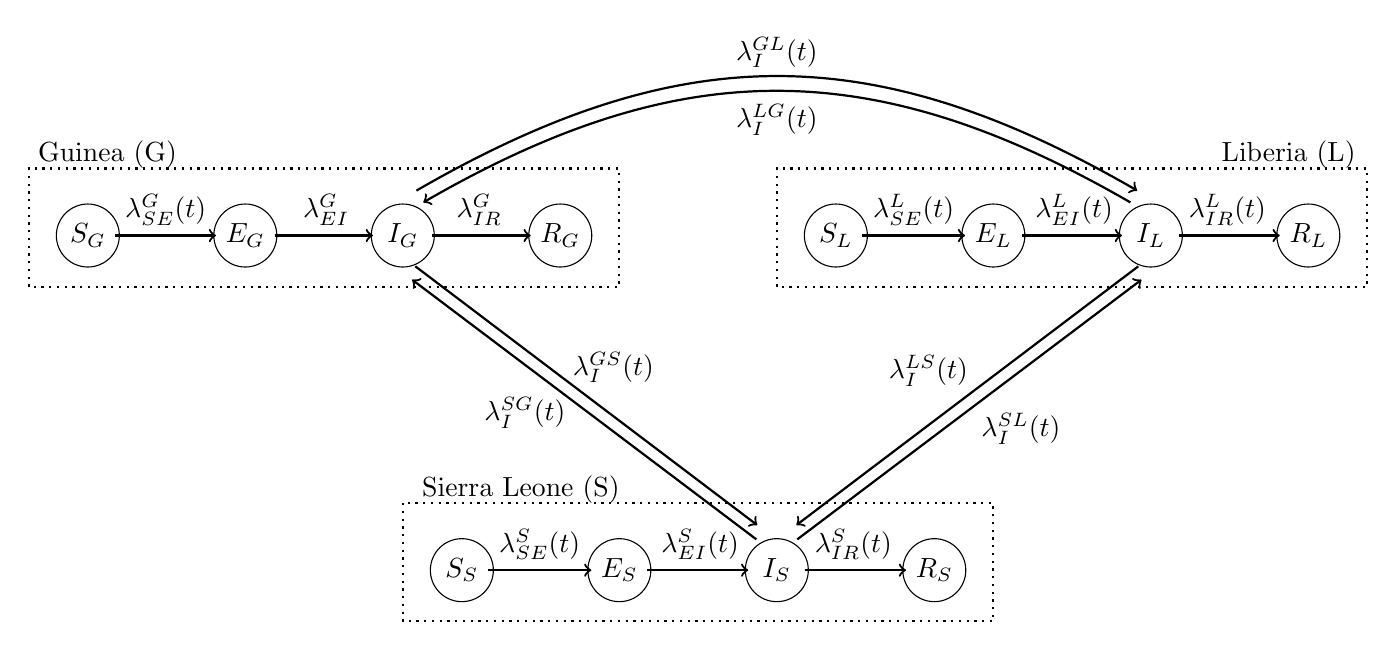
\begin{tikzpicture}
		\draw[thick,dotted] (0,-0.25) rectangle (7.5, 1.25);
		\node at (1, 1) [label=Guinea (G)] {};
		\draw (0.75, 0.4) circle(0.4) node (Sa) {$ S_G $};
		\draw (2.75, 0.4) circle(0.4) node (Ea) {$ E_G $};
		\draw (4.75, 0.4) circle(0.4) node (Ia) {$ I_G $};
		\draw (6.75, 0.4) circle(0.4) node (Ra) {$ R_G $};
		
		\draw[thick,dotted] (9.5,-0.25) rectangle (17, 1.25);
		\node at (16, 1) [label=Liberia (L)] {};	
		\draw (10.25, 0.4) circle(0.4) node (Sb) {$ S_L $};
		\draw (12.25, 0.4) circle(0.4) node (Eb) {$ E_L $};
		\draw (14.25, 0.4) circle(0.4) node (Ib) {$ I_L $};
		\draw (16.25, 0.4) circle(0.4) node (Rb) {$ R_L $};
		
		\draw[thick,dotted] (4.75,-3) rectangle (12.25, -4.5);
		\node at (6.25, -3.25) [label=Sierra Leone (S)] {};	
		\draw (5.5, -3.85) circle(0.4) node (Sc) {$ S_S $};
		\draw (7.5, -3.85) circle(0.4) node (Ec) {$ E_S $};
		\draw (9.5, -3.85) circle(0.4) node (Ic) {$ I_S $};
		\draw (11.5, -3.85) circle(0.4) node (Rc) {$ R_S $};
		
		\draw [thick,->] (Sa) -- (Ea) node[midway,above] {$ \lambda_{SE}^G(t) $};
		\draw [thick,->,shorten >=.6mm] (Ea) -- (Ia) node[midway,above] {$ \lambda_{EI}^G $};
		\draw [thick,->,shorten <=.5mm] (Ia) -- (Ra) node[midway,above] {$ \lambda_{IR}^G $};
		
		\draw [thick,->] (Sb) -- (Eb) node[midway,above] {$ \lambda_{SE}^L(t) $};
		\draw [thick,->,shorten >=.6mm] (Eb) -- (Ib) node[midway,above] {$ \lambda_{EI}^L(t) $};
		\draw [thick,->,shorten <=.5mm] (Ib) -- (Rb) node[midway,above] {$ \lambda_{IR}^L(t) $};
		
		\draw [thick,->] (Sc) -- (Ec) node[midway,above] {$ \lambda_{SE}^S(t) $};
		\draw [thick,->,shorten >=.6mm] (Ec) -- (Ic) node[midway,above] {$ \lambda_{EI}^S(t) $};
		\draw [thick,->,shorten <=.5mm] (Ic) -- (Rc) node[midway,above] {$ \lambda_{IR}^S(t) $};
		
		\path [thick, <-] ([yshift=-0.5mm,xshift=-2mm]Ia.south) edge [shorten >= 2mm, shorten <= 4mm] node [above,xshift=4.5mm,yshift=1.5mm] {$ \lambda_I^{GS}(t) $} ([xshift=-1mm]Ic.north);
		\path [thick, ->] (Ia.south) edge [shorten >= 5mm, shorten <= 2mm] node [below,xshift=-9mm,yshift=2mm] {$ \lambda_I^{SG}(t) $} ([xshift=1.5mm]Ic.north);
		
		\path [thick, <-] ([yshift=-0.5mm,xshift=2mm]Ib.south) edge [shorten >= 2mm, shorten <= 4mm] node[above,yshift=1mm,xshift=-6mm] {$ \lambda_I^{LS}(t) $} ([xshift=1mm]Ic.north);
		\path [thick, ->] (Ib.south) edge [shorten >= 5mm, shorten <= 2mm] node[below,xshift=8mm] {$ \lambda_I^{SL}(t) $} ([xshift=-1.5mm]Ic.north);
		
		\path [thick, <-] ([]Ia.north) edge [shorten >= 3mm, shorten <= 3mm, bend left, looseness=1.1] node [below] {$ \lambda_I^{LG}(t) $} ([]Ib.north);
		\path [thick, ->] ([]Ia.north) edge [shorten >= 2mm, shorten <= 2mm, bend left, looseness=1.1,yshift=2mm] node [above] {$ \lambda_I^{GL}(t) $} ([]Ib.north);		
		\end{tikzpicture}
	}
	\caption[Diagram for a stratified SEIR model with country specific outbreak dynamics and cross--country transmission.]{Diagram of state transitions for a stratified SEIR model used in simulating an outbreak in Guinea, Liberia, and Sierra Leone. Dashed boxes denote countries, nodes in circles denote the model compartments: susceptible (S), exposed (E), infectious (I), recovered (R). Compartments  are subscripted with country indicators. The number of susceptible individuals is equal to the effective population size, estimated as a parameter in the model, minus the numbers of exposed, infected, and recovered individuals. Solid lines with arrows indicate stochastic transitions between model compartments, which occur continuously in time. Rates at which individuals transition between compartments are denoted by $ \lambda $ and are subscripted by compartments and superscripted by countries, e.g., $ \lambda_{SE}^L $ is the rate at which susceptible individuals become exposed in Liberia, $ \lambda_I^{SG} $ is the rate at which an infected individual in Sierra Leone migrates to Guinea. The rate at which susceptible individuals in Guinea become infected is time varying with one changepoint at 33 weeks. Transmission in Liberia and Sierra Leone commenced at 10 and 19 weeks, respectively.Full expressions for the rates are given in Table \ref{tab:ebola_synth_rates_full}.}
	\label{fig:stratified_seir_full_diag}
\end{figure}

\begin{table}[htbp]
	\caption[Week zero, and true and effective population sizes for a simulated Ebola outbreak in West Africa.]{True and effective population sizes, and initial conditions for a simulated outbreak in Guinea, Liberia, and Sierra Leone. Week zero is one week before the first observation is accrued and the time at which within--country transmission was assumed to begin. }
	\label{tab:ebola_synth_consts}
	\footnotesize
	\centering
	\begin{tabular}{lccc}	
		\hline	
		& \textbf{Guinea} & \textbf{Liberia} & \textbf{Sierra Leone} \\\hline
		\textbf{True population size $ (N)$} & 11.8 million & 4.4 million & 7.1 million \\ 
		\textbf{Effective population size $ (N_{eff}) $} & 15,000 & 35,000 & 25,000 \\
		\textbf{Week zero $ (t_0) $} & 0 & 10 & 19 \\
		\textbf{Initial state at $ t_0 $} $ (S_0,E_0,I_0,R_0) $ & (11.8$ \times 10^6$-7, 4, 3, 0) & (4.4$ \times 10^6$-5 3, 2, 0)& (7.1$ \times 10^6$-5, 3, 2, 0) \\
		\hline
		&&&
	\end{tabular} 
\end{table}

\begin{sidewaystable}[htbp]
	\begin{fullpage}
		\caption[Parameters and priors for a simulated Ebola outbreak in West Africa.]{Parameters used to simulate an Ebola outbreak in West Africa using a country--stratified SEIR model, prior distributions, and 95\% prior intervals. Subscripts, $ G,L,S, $ indicate specific countries, or generic countries $ A,B $ if a prior is shared. Effective reproduction numbers are defined with respect to the effective population size as $ R_{eff} = \beta N_{eff} /\mu $.}
		\label{tab:ebola_synth_pars}
		\scriptsize
	\centering
	\begin{tabular}{lcllr}
		\hline
		\textbf{Parameter} & \textbf{Truth} & \textbf{Interpretation} & \textbf{Prior} & \textbf{Median (95\% Interval)} \\ \hline
		$ R_{eff,G}^{(1)}(t),\ t<33 $ & 1.3 & Effective reproduction \#  & $ R_{eff,G}^{(2)} / R_G^{(1)}\sim $ LogNormal(0, 0.5$ ^2 $) & $ R_{eff,G}^{(2)} / R_{eff,G}^{(1)} = $ 1.00 (0.38, 2.66) \\
		$ R_{eff,G}^{(2)}(t),\ t\geq33 $ & 1.2 & Effective reproduction \# & $ R_{eff,G}^{(2)}-1\sim $ LogNormal(log(0.5), 1.1) & $ \implies R_{eff,G}^{(2)} = 1.50 (1.06, 5.32)$ \\
		$ R_{eff,L} $ & 2.0 & Effective reproduction \# & $ R_{eff,L}\sim $ LogNormal(log(0.5), 1.1) & $ \implies R_{eff,L} = 1.50 (1.06, 5.32)$ \\
		$ R_{eff,S} $ & 1.55 & Effective reproduction \# & $ R_{eff,S}\sim $ LogNormal(log(0.5), 1.1) & $ \implies R_{eff,S} = 1.50 (1.06, 5.32)$ \\
		\makecell[l]{$ \alpha_{GS},\alpha_{GL}, \alpha_{LG},$\\
		$ \alpha_{LS},\alpha_{SG}, \alpha_{SL} $} & 0.003 & \makecell[l]{Infectious migration rate \\ from country A to B} & $ 1000\alpha_{AB} \sim$ Exponential(0.25) & \makecell[r]{\# migrations per 1000 infected \\ = 2.78 (0.10, 14.76)}\\ 
		$ \omega_G $ & 1.1 & Rate from $ E_G\rightarrow I_G $ & $ (1/\mu_G)\big/(1/\omega_G) \sim $ LogNormal(0.0, 0.3$ ^2 $) & $ (1/\mu_G)\big/(1/\omega_G) $ = 1.00 (0.56, 1.80) \\
		$ \omega_L $ & 0.85 & Rate from $ E_L\rightarrow I_L $ & $ (1/\mu_L)\big/(1/\omega_L) \sim $ LogNormal(0.0, 0.3$ ^2 $) & $ (1/\mu_L)\big/(1/\omega_L) $ = 1.00 (0.56, 1.80) \\
		$ \omega_S $ & 1 & Rate from $ E_S\rightarrow I_S $ & $ (1/\mu_S)\big/(1/\omega_S) \sim $ LogNormal(0.0, 0.3$ ^2 $) & $ (1/\mu_S)\big/(1/\omega_S) $ = 1.00 (0.56, 1.80) \\
		$ \mu_G $ & $ 1 $ & Rate from $ E_G\rightarrow I_G $ & $ 1/\mu_G\sim $ LogNormal(0, 0.25$ ^2 $) & $ 7/\mu_G = $ 7.0 (4.29, 11.43) \\
		$ \mu_L $ & $ 0.8 $ & Rate from $ E_L\rightarrow I_L $ & $ 1/\mu_L\sim $ LogNormal(0, 0.25$ ^2 $) & $ 7/\mu_L = $ 7.0 (4.29, 11.43) \\
		$ \mu_S $ & $ 1.1 $ & Rate from $ E_S\rightarrow I_S $ & $ 1/\mu_S\sim $ LogNormal(0, 0.25$ ^2 $) & $ 7/\mu_S = $ 7.0 (4.29, 11.43) \\
		$ N_{eff,G} $ & 15,000 & Effective population size & $ N_{eff,G}\sim\mr{Unif}(\sum_{\ell=1}^{L}Y_\ell^G, N_G/4) $& $ N_{eff,G} \in (4032,\ 2.95\times10^6) $ \\
		$ N_{eff,L} $ & 35,000 & Effective population size & $ N_{eff,L}\sim\mr{Unif}(\sum_{\ell=1}^{L}Y_\ell^L, N_L/4) $& $ N_{eff,L} \in (5945,\ 1.1\times10^6) $ \\
		$ N_{eff,S} $ & 25,000 & Effective population size & $ N_{eff,S}\sim\mr{Unif}(\sum_{\ell=1}^{L}Y_\ell^S, N_S/4) $& $ N_{eff,S} \in (9531,\ 1.775\times10^6) $ \\
		$ \rho_G $ & 0.85 & Mean case detection prob. & $ \logit(\rho_G) \sim $ LogNormal(0, 1.4$ ^2 $) & $ \implies \rho_G = 0.5, (0.06, 0.94)$ \\
		$ \rho_L $ & 0.25 & Mean case detection prob. & $ \logit(\rho_L) \sim $ LogNormal(0, 1.4$ ^2 $) & $ \implies \rho_L = 0.5, (0.06, 0.94)$ \\
		$ \rho_S $ & 0.55 & Mean case detection prob. & $ \logit(\rho_S) \sim $ LogNormal(0, 1.4$ ^2 $) & $ \implies \rho_S = 0.5, (0.06, 0.94)$ \\
		$ \phi_G,\ \phi_L, \phi_S $ & 50 & Neg.Binomial overdispersion & $ \log(\phi) \sim $ LogNormal(0, 5$ ^2 $) & $ \implies \rho_G = 1, (5.5\times 10^-5, 1.8\times10^4)$ \\
		\hline
	\end{tabular}
	\end{fullpage}
\end{sidewaystable}

\begin{table}[htbp]
	\caption[Priors for initial compartment volumes for a simulated Ebola outbreak in West Africa]{Priors for the initial compartment volumes at the times when transmission commenced in each country for a simulated Ebola outbreak in West Africa. The initial compartment volumes for each country are assigned independent truncated multivariate normal priors that respect the boundary conditions on the state space of compartment volumes for that country (explained in Section \ref{sec:lna_init_volumes}). If the population size for country A is $ N_A $, and the initial state probability is denoted $ \bp_{0,A} = \bX_{0,A}/N_A  = (S_{0,A}, E_{0,A}, I_{0,A}, R_{0,A})/N_A$, the prior is a truncated multivariate normal approximation of a multinomial distribution with mean $ N_A\bp_{0,A}$ and covariance $ N_A(\bP_{0,A} - \bp_{0,A}\bp_{0,A}^T) $.} 
	\label{tab:ebola_synth_initdist_priors}
	\centering
	\begin{tabular}{lc}
		\hline \textbf{Country} & \textbf{Prior mean initial volumes} ($ \bX_0 $) \\
		\hline
		Guinea & ($ 11.8\times10^6 -7.1$, 4, 3, 0.1) \\
		Liberia & ($ 4.4\times10^6 -5.1$, 3, 2, 0.1) \\
		Sierra Leone & ($ 7.1\times10^6 -5.1$, 3, 2, 0.1) \\
		\hline
	\end{tabular}
\end{table}

\begin{table}[htbp]
	\caption[Transmission rates for the stratified SEIR model with migration of infecteds for Ebola in West Africa.]{Rates of transitions between compartments for the full stratified SEIR model for the spread of Ebola in Guinea, Liberia, and Sierra Leone with cross--country migration of infected individuals across country borders. These rates were used in simulating the outbreak and data, and in the supplementary model presented in Section \ref{subsec:ebola_synth_fullmod_res}. The model is diagrammed in Figure \ref{fig:stratified_seir_full_diag}. Subscripts in the rates denote model compartments, superscripts denote countries. Subscripts for parameters denote countries. The number of susceptible individuals is equal to the effective population size, estimated as a parameter in the model, minus the numbers of exposed, infected, and recovered individuals. The rate at which susceptibles in Guine become infected is time varying with one changepoint at 33 weeks. Transmission in Liberia and Sierra Leone prior to weeks 10 and 19 is expressed in the initial compartment volumes at those times. Thus, all respective transition rates are set to zero prior to the times when transmission commenced in those countries.}
	\label{tab:ebola_synth_rates_full}
	\centering\footnotesize
	\begin{tabular}{llll}
		\hline
		\textbf{From} & \textbf{To} & \textbf{Country} & \textbf{Rate} \\
		\hline
		Susceptible & Exposed & Guinea & $ \lambda_{SE}^G(t) = (\beta_G^{(1)} \ind{t<33} + \beta_G^{(2)}\ind{t\geq33})S_GI_G $ \\
		Susceptible & Exposed & Liberia & $ \lambda_{SE}^L(t) = \beta_LS_LI_L\ind{t\geq10} $\\
		Susceptible & Exposed & Sierra Leone & $ \lambda_{SE}^S(t) = \beta_SS_SI_S\ind{t\geq19} $ \\
		Exposed & Infected & Guinea & $ \lambda_{EI}^G = \omega_GE_G $\\
		Exposed & Infected & Liberia & $ \lambda_{EI}^L(t) = \omega_LE_L\ind{t\geq10} $ \\
		Exposed & Infected & Sierra Leone & $\lambda_{EI}^S(t) = \omega_SE_S\ind{t\geq19}$ \\
		Infected & Recovered & Guinea & $ \lambda_{IR}^G = \mu_GI_G $ \\
		Infected & Recovered & Liberia & $ \lambda_{IR}^L(t) = \mu_LI_L\ind{t\geq10} $ \\	
		Infected & Recovered & Sierra Leone & $ \lambda_{IR}^S(t) = \mu_SI_S\ind{t\geq19} $ \\
		Infected (A) & Infected (B) & Countries A,B & $ \lambda_I ^{AB}(t) = \alpha_{AB}I_A\ind{t\geq{t_{0}^A}}\ind{t\geq t_{0}^B}$\\
		\hline
	\end{tabular}
\end{table}

\begin{table}[htbp]
	\caption[Transmission rates for the stratified SEIR model with virtual migration of infecteds for Ebola in West Africa.]{Approximate rates of transitions between compartments for the stratified SEIR model for the spread of Ebola in Guinea, Liberia, and Sierra Leone with cross--country transmission via virtual migration of infected individuals. These rates were used in the primary model presented in Section \ref{subsec:ebola_synth}. The model is diagrammed in Figure \ref{fig:stratified_seir_full_diag}. Subscripts in the rates denote model compartments, superscripts denote countries. Subscripts for parameters denote countries. The number of susceptible individuals is equal to the effective population size, estimated as a parameter in the model, minus the numbers of exposed, infected, and recovered individuals. The rate at which susceptibles in Guine become infected is time varying with one changepoint at 33 weeks. Transmission in Liberia and Sierra Leone prior to weeks 10 and 19 is expressed in the initial compartment volumes at those times. Thus, all respective transition rates are set to zero prior to the times when transmission commenced in those countries.}
	\label{tab:ebola_synth_rates_approx}
	\centering\footnotesize
	\begin{tabular}{llll}
		\hline
		\textbf{From} & \textbf{To} & \textbf{Country} & \textbf{Rate} \\
		\hline
		Susceptible & Exposed & Guinea & \hspace{-0.7in}\makecell{$ \lambda_{SE}^G(t) = (\beta_G^{(1)} \ind{t<33} + \beta_G^{(2)}\ind{t\geq33})\times $\\
		\hspace{1.25in}$ (I_G + \alpha_{LG}I_L\ind{t\geq10} + \alpha_{SG}I_S\ind{t\geq19})S_G $}\\
		Susceptible & Exposed & Liberia & $ \lambda_{SE}^L(t) = \beta_L(I_L + \alpha_{GL}I_G + \alpha_{SL}I_S\ind{t\geq19})S_L\ind{t\geq10} $\\
		Susceptible & Exposed & Sierra Leone & $ \lambda_{SE}^S(t) = \beta_S(I_S + \alpha_{GS}I_G + \alpha_{LS}I_L)S_S \ind{t\geq19} $ \\
		Exposed & Infected & Guinea & $ \lambda_{EI}^G = \omega_GE_G $\\
		Exposed & Infected & Liberia & $ \lambda_{EI}^L(t) = \omega_LE_L \ind{t\geq10}$ \\
		Exposed & Infected & Sierra Leone & $\lambda_{EI}^S(t) = \omega_SE_S\ind{t\geq19}$ \\
		Infected & Recovered & Guinea & $ \lambda_{IR}^G = \mu_GI_G $ \\
		Infected & Recovered & Liberia & $ \lambda_{IR}^L(t) = \mu_LI_L\ind{t\geq10} $ \\	
		Infected & Recovered & Sierra Leone & $ \lambda_{IR}^S(t) = \mu_SI_S\ind{t\geq19} $ \\
		\hline
	\end{tabular}
\end{table}

\newpage
\subsection{MCMC Details}
\label{subsec:ebola_synth_mcmc}
We fit two models to the simulated data, the true model where migration was modeled explicitly and the approximated model, described in Section \ref{subsec:ebola_synth}, where cross--border transmission was incorporated into the rate of infection via virtual migration. The model fitting procedure and priors were the same for both models. We ran five chains for each model, initialized at random parameter values, for 200,000 iterations per chain. The model parameters, not including the initial compartment volumes, were jointly updated via MVNSS (see Section \ref{subsubsec:mvn_slice_sampling}). The empirical covariance for the MVNSS algorithm was adapted over the first 100,000 iterations using the gain factor sequence, $\gamma_n = 0.5(1 + 0.01n)^{-0.9}$. The contribution of isotropic Gaussian noise to the proposal was initialized at 0.001 and reduced throughout the adaptation phase according to the sequence $ \iota_n = 0.001(1 + 0.01n)^{-0.99} $. The covariance matrix was blocked by country with covariances for parameters belonging to different countries set to zero. Thus, country specific parameters were proposed jointly but were independent in the proposal. Migration parameters were blocked with parameters corresponding to the destination country. The initial compartment volumes were updated jointly with the LNA paths in an EllipSS step. The MCMC alternated between three ElliptSS and two MVNSS updates per MCMC iteration. The ElliptSS bracket width was reset after the first 5,000 MCMC iterations to $ \omega = 2\sqrt{2\log(10)}\sigma_{ElliptSS}$, where $ \sigma_{ElliptSS} $ was the standard deviation of the accepted angles over the initial iterations. The MCMC estimation scales for each country were parameterized as in Table \ref{tab:seir_params_est3} with the one addition being the log ratio of effective reproductive numbers, subtract one, for Guinea, $ \log\left ((R_{eff,G}^{(2)}-1)/(R_{eff,G}^{(1)}-1)\right ) $. Convergence was assessed visually by inspection of traceplots of posterior samples, and via potential scale reduction factors (PSRFs) \cite{brooks1998general} computed via the \texttt{coda} R package \cite{codapackage}. The full model took approximately 9.6 days to run, while the approximate model took about 2.8 days. 

\subsection{Additional Results}
\label{subsec:ebola_synth_supplement}

\begin{table}[htbp]
	\caption[Posterior estimates of initial numbers of exposed, infected, and recovered individuals for a stratified SEIR model fit to simulated Ebola data.]{Posterior estimates of initial numbers of exposed, infected, and recovered individuals for a stratified approximate SEIR model with virtual migration of infecteds fit to simulated Ebola data. The effective number of susceptibles is equal to the effective population size, reported in Table \ref{tab:ebola_synth_ests}, minus the numbers of exposed, infected, and recovered individuals, but is not reported since the effective population size is not marginally identifiable.}
	\label{tab:ebola_synth_initdist_res}
	\centering
	\begin{tabular}{lrl}
		\hline
		\textbf{Parameter} & \textbf{Truth} & \textbf{Estimate} \\ 
		\hline
		$ E_{0,G} $& 4.00 & 4.99 (1.39, 8.66) \\ 
		$ E_{0,G} $& 3.00 & 3.4 (0.6, 6.76) \\ 
		$ E_{0,G} $& 3.00 & 3.16 (0.45, 6.55) \\ 
		$ I_{0,G} $& 3.00 & 3.7 (0.82, 6.91) \\ 
		$ I_{0,L} $& 2.00 & 2.67 (0.45, 5.23) \\ 
		$ I_{0,S} $& 2.00 & 2.46 (0.4, 4.95) \\ 
		$ R_{0,G} $& 0.00 & 0.12 (0.07, 0.16) \\ 
		$ R_{0,L} $	& 0.00 & 0.12 (0.07, 0.17) \\ 
		$ R_{0,S} $& 0.00 & 0.11 (0.06, 0.17) \\ 
		\hline
	\end{tabular}
\end{table}

\begin{table}[htbp]
	\caption[Posterior parameter estimates for full and approximate stratified SEIR models fit to a simulated Ebola outbreak.]{Posterior medians (95\% Bayesian credible intervals) for parameters of the full (Figure \ref{fig:stratified_seir_full_diag}) and approximate (Figure \ref{fig:stratified_seir_approx_diag}) stratified SEIR models fit to a simulated Ebola outbreak. The full model explicitly models cross--border transmission via migration of infected individuals, while the approximate model incorporates cross--border transmission through virtual migrations. Subscripts, $ G,L,S, $ indicate specific countries, or generic countries $ A,B $. Effective reproduction numbers are defined with respect to the effective population size as $ R_{eff} = \beta N_{eff} /\mu $. Parameter interpretations and priors are given in Table \ref{tab:ebola_synth_pars}.}
	\label{tab:ebola_synth_ests}
	\centering\footnotesize
	\begin{tabular}{ccrr}		
		\hline
		& & \multicolumn{2}{c}{\textbf{Posterior median (95\% BCI)}}\\\cline{3-4}
		\textbf{Parameter} & \textbf{Truth} & \textit{Approximate Model} & \textit{Full Model} \\ 
		\hline
		$ R_{eff,G}^{(1)} $& 1.30 & 1.24 (1.12, 1.44) & 1.23 (1.13, 1.43) \\ 
		$ R_{eff,G}^{(2)} $& 1.20 & 1.28 (1.1, 1.63)& 1.27 (1.13, 1.52) \\ 
		$ R_{eff,L} $& 2.00 & 1.69 (1.37, 2.22) & 2.07 (1.56, 3.06)  \\ 
		$ R_{eff,S} $& 1.55 & 1.54 (1.31, 1.97)& 1.52 (1.31, 1.91) \\ 
		$ 7/\omega_G $& 6.36 & 5.55 (2.92, 10.44)& 3.78 (1.89, 8.21)  \\ 
		$ 7/\omega_L $& 8.24 & 6 (2.78, 11.2)&  8.28 (3.87, 15.19) \\ 
		$ 7/\omega_S $& 7.00 & 6.14 (3.26, 11.22)& 5.67 (2.98, 10.58) \\ 
		$ 7/\mu_G $& 7.00 & 6.19 (4.06, 9.65)& 5.83 (3.46, 9.85) \\ 
		$ 7/\mu_L $ & 8.75 & 6.41 (4.05, 9.95) & 8.96 (5.3, 14.7) \\
		$ 7/\mu_S $& 6.36 & 6.46 (4.17, 10.04)& 6.55 (4.25, 9.89) \\ 
		$ 1000\alpha_{GL} $& 3.00 & 3.46 (0.13, 17.22) & 16.22 (6.32, 35.08) \\ 
		$ 1000\alpha_{GS} $& 3.00 & 3.75 (0.14, 18.93)& 20.8 (8.14, 43.62) \\ 
		$ 1000\alpha_{LG} $& 3.00 & 2.19 (0.12, 8.33)&  8.72 (3.29, 19.35) \\ 
		$ 1000\alpha_{LS} $& 3.00 & 3.03 (0.22, 11.3) & 10.15 (3.44, 22.94)  \\ 
		$ 1000\alpha_{SG} $& 3.00 & 2.96 (0.16, 13.67)&  10.05 (3.46, 22.77) \\ 
		$ 1000\alpha_{SL} $& 3.00 & 2.69 (0.12, 11.51)& 5.58 (2.02, 14.79) \\ 
		$ \rho_GN_{eff,G} $& 12750 & 11570 (7750, 19320) &  11590 (7500, 19560) \\ 
		$ \rho_LN_{eff,L} $& 8750 & 10030 (8070, 14180)& 8560 (7220, 11420) \\ 
		$ \rho_SN_{eff,S} $& 15000 & 14860 (11510, 20580)& 15420 (11740, 21230) \\ 
		$ \phi_{G} $& 50.00 & 59.78 (27.36, 211.88) & 42.87 (22.15, 96.72) \\ 
		$ \phi_{L} $& 50.00 & 46.61 (20.82, 105.31)& 46.62 (20.77, 101.46) \\ 
		$ \phi_{S} $& 50.00 & 33.13 (17.76, 60.48) & 31.02 (16.93, 55.48) \\
		\hline
	\end{tabular}
\end{table}

\begin{table}[htbp]
	\caption{Effective sample sizes and potential scale reduction factors for the stratified SEIR model with virtual migration of infecteds fit to a simulated Ebola outbreak.}
	\centering
	\begin{tabular}{lrr}
		\hline
		\textbf{Parameter} & \textbf{ESS} & \textbf{PSRF} \\ 
		\hline
		$ \log\left (R_{eff,G}^{(2)} / R_{eff,G}^{(1)}\right ) $& 461 & 1.01 \\ 
		$ \log\left (R_{eff,G}^{(2)}\right ) $& 367 & 1.01 \\ 
		$ \log\left (R_{eff,L}\right ) $& 505 & 1.06 \\ 
		$ \log\left (R_{eff,S}\right ) $& 759 & 1.02 \\ 
		$ \log\left (\omega_G / \mu_G\right ) $& 1057 & 1.00 \\ 
		$ \log\left (\omega_L / \mu_L\right ) $& 664 & 1.05 \\ 
		$ \log\left (\omega_S / \mu_S\right ) $& 851 & 1.01 \\ 
		$ \log\left (1/\mu_G\right ) $& 719 & 1.01 \\ 
		$ \log\left (1/\mu_L\right ) $& 692 & 1.04 \\ 
		$ \log\left (1/\mu_S\right ) $& 1038 & 1.01 \\ 
		$ \log\left (1000\alpha_{GL}\right ) $& 712 & 1.03 \\ 
		$ \log\left (1000\alpha_{GS}\right ) $& 813 & 1.04 \\ 
		$ \log\left (1000\alpha_{LG}\right ) $& 344 & 1.13 \\ 
		$ \log\left (1000\alpha_{LS}\right ) $& 539 & 1.09 \\ 
		$ \log\left (1000\alpha_{SG}\right ) $& 494 & 1.03 \\ 
		$ \log\left (1000\alpha_{SL}\right ) $& 641 & 1.10 \\ 
		$ \log\left (\rho_GN_{eff,G}\right ) $& 525 & 1.00 \\ 
		$ \log\left (\rho_LN_{eff,L}\right ) $& 603 & 1.08 \\ 
		$ \log\left (\rho_SN_{eff,S}\right ) $& 1020 & 1.01 \\ 
		$ \logit\left (\rho_G\right ) $& 445 & 1.01 \\ 
		$ \logit\left (\rho_L\right ) $& 354 & 1.04 \\ 
		$ \logit\left (\rho_S\right ) $& 540 & 1.03 \\ 
		$ \log(\phi_G) $& 479 & 1.08 \\ 
		$ \log(\phi_L) $& 999 & 1.00 \\ 
		$ \log(\phi_S) $& 1012 & 1.01 \\ 
		\hline
	\end{tabular}
\end{table}

\begin{sidewaysfigure}[htbp]
	\centering
	\includegraphics[width=\linewidth]{figures/ebola_synth_traces}
	\caption{Posterior traceplots for a stratified SEIR model fit to a simulated Ebola outbreak.}
	\label{fig:ebolasynthtraces}
\end{sidewaysfigure}

\begin{figure}[htbp]
	\centering
	\includegraphics[width=\linewidth]{figures/ebola_synth_pairs_guin}
	\caption{Scatterplots of Guinea--specific parameters in a stratified SEIR model for a simulated Ebola outbreak.}
\end{figure}

\begin{figure}[htbp]
	\centering
	\includegraphics[width=\linewidth]{figures/ebola_synth_pairs_lib}
	\caption{Scatterplots of Liberia--specific parameters in a stratified SEIR model for a simulated Ebola outbreak.}
\end{figure}

\begin{figure}[htbp]
	\centering
	\includegraphics[width=\linewidth]{figures/ebola_synth_pairs_sln}
	\caption{Scatterplots of Sierra Leone--specific parameters in a stratified SEIR model for a simulated Ebola outbreak.}
\end{figure}

\newpage
\section{Modeling Ebola in West Africa --- MCMC Details and Supplementary Results}
\label{sec:ebola_supplement}

\subsection{Details and Supplementary Results for Single--Country Models}
\label{subsec:ebola_single_country_supplement}


\begin{table}[htbp]
	\caption[Transmission rates for single country SEIR models for Ebola in West Africa.]{Rates of transitions between compartments of single country SEIR models, diagrammed in Figure \ref{fig:ebola_single_diag}, for the spread of Ebola in Guinea, Liberia, and Sierra Leone with constant rate of infectious contact from outside the population. Subscripts in the rates denote model compartments, superscripts denote countries. Subscripts for parameters denote countries. The number of susceptible individuals is equal to the effective population size, estimated as a parameter in the model, minus the numbers of exposed, infected, and recovered individuals. The rate at which susceptibles in Guine become infected is time varying with one changepoint at 33 weeks. Transmission in Liberia and Sierra Leone prior to weeks 10 and 19 is expressed in the initial compartment volumes at those times, but is not modeled explicitly.}
	\label{tab:ebola_rates_single}
	\centering\footnotesize
	\begin{tabular}{llll}
		\hline
		\textbf{From} & \textbf{To} & \textbf{Country} & \textbf{Rate} \\
		\hline
		Susceptible & Exposed & Guinea & $ \lambda_{SE}^G(t) = \left (\alpha_G + (\beta_G^{(1)} \ind{t<33} + \beta_G^{(2)}\ind{t\geq33})I_G\right )S_G $ \\
		Susceptible & Exposed & Liberia & $ \lambda_{SE}^L = \left (\alpha_L + \beta_LI_L\right )S_L $\\
		Susceptible & Exposed & Sierra Leone & $ \lambda_{SE}^S = \left (\alpha_S + \beta_SI_S\right )S_S $ \\
		Exposed & Infected & Guinea & $ \lambda_{EI}^G = \omega_GE_G $\\
		Exposed & Infected & Liberia & $ \lambda_{EI}^L(t) = \omega_LE_L $ \\
		Exposed & Infected & Sierra Leone & $\lambda_{EI}^S = \omega_SE_S$ \\
		Infected & Recovered & Guinea & $ \lambda_{IR}^G = \mu_GI_G $ \\
		Infected & Recovered & Liberia & $ \lambda_{IR}^L = \mu_LI_L $ \\	
		Infected & Recovered & Sierra Leone & $ \lambda_{IR}^S = \mu_SI_S$ \\
		\hline
	\end{tabular}
\end{table}

\subsubsection{Priors and MCMC details}
\label{subsubsec:ebola_single_mcmc}

We fit country specific SEIR models to the Ebola incidence data from Guinea, Liberia, and Sierra Leone under two prior regimes given in Tables \ref{tab:ebola_priors_single_tight} and \ref{tab:ebola_priors_single_diff}. The model fitting procedure and priors were the same for all models. We ran five chains for each model, initialized at random parameter values, for 200,000 iterations per chain. The model parameters, not including the initial compartment volumes, were jointly updated via MVNSS (see Section \ref{subsubsec:mvn_slice_sampling}). The empirical covariance for the MVNSS algorithm was adapted over the first 100,000 iterations using the gain factor sequence, $\gamma_n = 0.5(1 + 0.01n)^{-0.9}$. The contribution of isotropic Gaussian noise to the proposal was initialized at 0.001 and reduced throughout the adaptation phase according to the sequence $ \iota_n = 0.001(1 + 0.01n)^{-0.99} $. The initial compartment volumes were updated jointly with the LNA paths in an EllipSS step. The MCMC alternated between two ElliptSS and one MVNSS update per MCMC iteration. The ElliptSS bracket width was reset after the first 5,000 MCMC iterations to $ \omega = 2\sqrt{2\log(10)}\sigma_{ElliptSS}$, where $ \sigma_{ElliptSS} $ was the standard deviation of the accepted angles over the initial iterations. The MCMC estimation scales for each country were parameterized as in Table \ref{tab:seir_params_est3} with the one addition being the log ratio of effective reproductive numbers, subtract one, for Guinea, $ \log\left ((R_{eff,G}^{(2)}-1)/(R_{eff,G}^{(1)}-1)\right ) $. Convergence was assessed visually by inspection of traceplots of posterior samples, and via potential scale reduction factors (PSRFs) \cite{brooks1998general} computed via the \texttt{coda} R package \cite{codapackage}. The models took between 8 hours and 34 hours to run, depending on the speed of the cluster cores. 

\begin{table}[htbp]
	\caption[Priors for initial compartment volumes for single country models fit to data from the Ebola outbreak in West Africa.]{Priors for the initial compartment volumes at the times when transmission commenced in each country for single country models fit to data from the Ebola outbreak in West Africa. The initial compartment volumes for each country are assigned independent truncated multivariate normal priors that respect the boundary conditions on the state space of compartment volumes for that country (explained in Section \ref{sec:lna_init_volumes}). If the population size for country A is $ N_A $, and the initial state probability is denoted $ \bp_{0,A} = \bX_{0,A}/N_A  = (S_{0,A}, E_{0,A}, I_{0,A}, R_{0,A})/N_A$, the prior is a truncated multivariate normal approximation of a multinomial distribution with mean $ N_A\bp_{0,A}$ and covariance $ N_A(\bP_{0,A} - \bp_{0,A}\bp_{0,A}^T) $.} 
	\label{tab:ebola_single_initdist_priors}
	\centering
	\begin{tabular}{lc}
		\hline \textbf{Country} & \textbf{Prior mean initial volumes} ($ \bX_0 $) \\
		\hline
		Guinea & ($ 11.8\times10^6 -7.1$, 4, 3, 0.1) \\
		Liberia & ($ 4.4\times10^6 -5.1$, 3, 2, 0.1) \\
		Sierra Leone & ($ 7.1\times10^6 -5.1$, 3, 2, 0.1) \\
		\hline
	\end{tabular}
\end{table}

\begin{sidewaystable}[htbp]
	\begin{fullpage}
		\caption[Parameters and priors for single country SEIR models fit to the West Africa Ebola outbreak.]{Parameters for a single country SEIR models fit to the West Africa Ebola outbreak, prior distributions used in the main analysis, 95\% prior intervals, and references that informed the choice of priors. Subscripts, $ G,L,S, $ indicate specific countries, or generic countries $ A,B $ if a prior is shared. Effective reproduction numbers are defined with respect to the effective population size as $ R_{eff} = \beta N_{eff} /\mu $.}
		\label{tab:ebola_priors_single_tight}
		\scriptsize
		\centering
		\begin{tabular}{lllrr}
			\hline
			\textbf{Parameter} &  \textbf{Interpretation} & \textbf{Prior} & \textbf{Median (95\% Interval)} & \textbf{References} \\ \hline
			$ R_{eff,G}^{(2)} / R_{eff,G}^{(1)} $ & Ratio of effective reproduction \#s &  LogNormal(0, 0.5$ ^2 $) & $ R_{eff,G}^{(2)} / R_{eff,G}^{(1)} = $ 1.00 (0.38, 2.66) & \cite{chowell2014transmission,chretien2015mathematical,coltart2017ebola,king2015avoidable} \\
			$ R_{eff,G}^{(2)}(t)-1 $ & Effective reproduction \# - 1, $ t\geq33 $ & LogNormal(log(0.5), $ 0.75^2 $) & $ \implies R_{eff,G}^{(2)} = 1.50 (1.11, 3.17)$ &  \cite{chowell2014transmission,chretien2015mathematical,coltart2017ebola,king2015avoidable} \\
			$ R_{eff,L} -1 $ & Effective reproduction \#-1 &  LogNormal(log(0.5), $ 0.75^2 $) & $ \implies R_{eff,L} = 1.50 (1.11, 3.17)$ &  \cite{chowell2014transmission,chretien2015mathematical,coltart2017ebola,king2015avoidable} \\
			$ R_{eff,S}-1 $ & Effective reproduction \#-1 & LogNormal(log(0.5), 0.75$ ^2 $) & $ \implies R_{eff,S} = 1.50 (1.11, 3.17)$ &  \cite{chowell2014transmission,chretien2015mathematical,coltart2017ebola,king2015avoidable}\\
			$ \alpha_{G},\alpha_{L}, \alpha_{S}$ & \makecell[l]{Rate of infectious contact \\ from outside the country} & $ 1000\alpha_{A} \sim$ Exponential(0.25) & \makecell[r]{\# migrations per 1000 infected \\ = 2.78 (0.10, 14.76)} & \cite{dudas2017virus}\\ 
			$ \omega_G/\omega_G $ & Rate from $ E_G\rightarrow I_G $ & LogNormal(0.0, 0.3$ ^2 $) & $ (1/\mu_G)\big/(1/\omega_G) $ = 1.00 (0.56, 1.80) & \cite{chowell2014transmission,velasquez2015time,glynn2017variability} \\
			$ \omega_L/\omega_L $ & Rate from $ E_L\rightarrow I_L $ & LogNormal(0.0, 0.3$ ^2 $) & $ (1/\mu_L)\big/(1/\omega_L) $ = 1.00 (0.56, 1.80) & \cite{chowell2014transmission,velasquez2015time,glynn2017variability} \\
			$ \omega_S/\omega_S $ & Rate from $ E_S\rightarrow I_S $ & LogNormal(0.0, 0.3$ ^2 $) & $ (1/\mu_S)\big/(1/\omega_S) $ = 1.00 (0.56, 1.80) & \cite{chowell2014transmission,velasquez2015time,glynn2017variability} \\
			$ 1/\mu_G $ & Rate from $ E_G\rightarrow I_G $ &  LogNormal(0.3, 0.2$ ^2 $) & $ 7/\mu_G = $ 9.45 (6.38, 13.98) & \cite{chowell2014transmission,velasquez2015time,glynn2017variability} \\
			$ 1/\mu_L $ & Rate from $ E_L\rightarrow I_L $ &  LogNormal(0.3, 0.2$ ^2 $) & $ 7/\mu_L = $ 9.45 (6.38, 13.98) & \cite{chowell2014transmission,velasquez2015time,glynn2017variability} \\
			$ 1/\mu_S $ & Rate from $ E_S\rightarrow I_S $ &  LogNormal(0.3, 0.2$ ^2 $) & $ 7/\mu_S = $ 9.45 (6.38, 13.98) & \cite{chowell2014transmission,velasquez2015time,glynn2017variability} \\
			$ N_{eff,G} $ & Effective population size & $\mr{Unif}(\sum_{\ell=1}^{L}Y_\ell^G, N_G/4) $& $ N_{eff,G} \in (3627,\ 2.95\times10^6) $ & Scale of counts \\
			$ N_{eff,L} $ & Effective population size & $\mr{Unif}(\sum_{\ell=1}^{L}Y_\ell^L, N_L/4) $& $ N_{eff,L} \in (4994,\ 1.1\times10^6) $ & Scale of counts \\
			$ N_{eff,S} $ & Effective population size & $\mr{Unif}(\sum_{\ell=1}^{L}Y_\ell^S, N_S/4) $& $ N_{eff,S} \in (11317,\ 1.775\times10^6) $ & Scale of counts \\
			$ \rho_G $ &  Mean case detection prob. & LogitNormal(0, 1.4$ ^2 $) & $ \implies \rho_G = 0.5, (0.06, 0.94)$ & Very high and very low $ \rho $ unlikely. \\
			$ \rho_L $ &  Mean case detection prob. & LogitNormal(0, 1.4$ ^2 $) & $ \implies \rho_L = 0.5, (0.06, 0.94)$ & Very high and very low $ \rho $ unlikely. \\
			$ \rho_S $ & Mean case detection prob. & LogitNormal(0, 1.4$ ^2 $) & $ \implies \rho_S = 0.5, (0.06, 0.94)$ & Very high and very low $ \rho $ unlikely. \\
			$ \phi_G,\ \phi_L, \phi_S $ &  Neg.Binomial overdispersion & LogNormal(0, 5$ ^2 $) & $ \implies \ = 1, (5.5\times 10^-5, 1.8\times10^4)$ & Diffuse. \\
			\hline
		\end{tabular}
	\end{fullpage}
\end{sidewaystable}

\begin{sidewaystable}[htbp]
	\begin{fullpage}
		\caption[Parameters and priors for supplementary single country SEIR models fit to the West Africa Ebola outbreak.]{Parameters for a single country SEIR models fit to the West Africa Ebola outbreak, prior distributions used in the supplementary analysis, 95\% prior intervals, and references that informed the choice of priors. Subscripts, $ G,L,S, $ indicate specific countries, or generic countries $ A,B $ if a prior is shared. Effective reproduction numbers are defined with respect to the effective population size as $ R_{eff} = \beta N_{eff} /\mu $. Prior distributions for parameters controlling the outbreak dynamics for the supplementary models were more diffuse vis--a--vis the priors in the main analysis.}
		\label{tab:ebola_priors_single_diff}
		\scriptsize
		\centering
		\begin{tabular}{lllrr}
			\hline
			\textbf{Parameter} &  \textbf{Interpretation} & \textbf{Prior} & \textbf{Median (95\% Interval)} & \textbf{References} \\ \hline
			$ R_{eff,G}^{(2)} / R_{eff,G}^{(1)} $ & Ratio of effective reproduction \#s &  LogNormal(0, 0.5$ ^2 $) & $ R_{eff,G}^{(2)} / R_{eff,G}^{(1)} = $ 1.00 (0.38, 2.66) & \cite{chowell2014transmission,chretien2015mathematical,coltart2017ebola,king2015avoidable} \\
			$ R_{eff,G}^{(2)}(t)-1 $ & Effective reproduction \# - 1, $ t\geq33 $ & LogNormal(log(0.5), $ 1.5^2 $) & $ \implies R_{eff,G}^{(2)} = 1.50 (1.02, 10.46)$ &  \cite{chowell2014transmission,chretien2015mathematical,coltart2017ebola,king2015avoidable} \\
			$ R_{eff,L} -1 $ & Effective reproduction \#-1 &  LogNormal(log(0.5), $ 1.5^2 $) & $ \implies R_{eff,L} = 1.50 (1.02, 10.46)$ &  \cite{chowell2014transmission,chretien2015mathematical,coltart2017ebola,king2015avoidable} \\
			$ R_{eff,S}-1 $ & Effective reproduction \#-1 & LogNormal(log(0.5), 1.5$ ^2 $) & $ \implies R_{eff,S} = 1.50 (1.02, 10.46)$ &  \cite{chowell2014transmission,chretien2015mathematical,coltart2017ebola,king2015avoidable}\\
			$ 1000\alpha_{A}$ & \makecell[l]{Rate of infectious contact \\ from outside  country A} & Exponential(0.125) & \makecell[r]{\# migrations per 1000 infected \\ = 5.55 (0.20, 29.51)} & \cite{dudas2017virus}\\ 
			$ \omega_G/\omega_G $ & Rate from $ E_G\rightarrow I_G $ & LogNormal(0.0, 0.3$ ^2 $) & $ (1/\mu_G)\big/(1/\omega_G) $ = 1.00 (0.56, 1.80) & \cite{chowell2014transmission,velasquez2015time,glynn2017variability} \\
			$ \omega_L/\omega_L $ & Rate from $ E_L\rightarrow I_L $ & LogNormal(0.0, 0.3$ ^2 $) & $ (1/\mu_L)\big/(1/\omega_L) $ = 1.00 (0.56, 1.80) & \cite{chowell2014transmission,velasquez2015time,glynn2017variability} \\
			$ \omega_S/\omega_S $ & Rate from $ E_S\rightarrow I_S $ & LogNormal(0.0, 0.3$ ^2 $) & $ (1/\mu_S)\big/(1/\omega_S) $ = 1.00 (0.56, 1.80) & \cite{chowell2014transmission,velasquez2015time,glynn2017variability} \\
			$ 1/\mu_G $ & Rate from $ E_G\rightarrow I_G $ &  LogNormal(0.3, 0.35$ ^2 $) & $ 7/\mu_G = $ 9.45 (4.76, 18.76) & \cite{chowell2014transmission,velasquez2015time,glynn2017variability} \\
			$ 1/\mu_L $ & Rate from $ E_L\rightarrow I_L $ &  LogNormal(0.3, 0.35$ ^2 $) & $ 7/\mu_L = $ 9.45 (4.76, 18.76) & \cite{chowell2014transmission,velasquez2015time,glynn2017variability} \\
			$ 1/\mu_S $ & Rate from $ E_S\rightarrow I_S $ &  LogNormal(0.3, 0.35$ ^2 $) & $ 7/\mu_S = $ 9.45 (4.76, 18.76) & \cite{chowell2014transmission,velasquez2015time,glynn2017variability} \\
			$ N_{eff,G} $ & Effective population size & $\mr{Unif}(\sum_{\ell=1}^{L}Y_\ell^G, N_G/4) $& $ N_{eff,G} \in (3627,\ 2.95\times10^6) $ & Scale of counts \\
			$ N_{eff,L} $ & Effective population size & $\mr{Unif}(\sum_{\ell=1}^{L}Y_\ell^L, N_L/4) $& $ N_{eff,L} \in (4994,\ 1.1\times10^6) $ & Scale of counts \\
			$ N_{eff,S} $ & Effective population size & $\mr{Unif}(\sum_{\ell=1}^{L}Y_\ell^S, N_S/4) $& $ N_{eff,S} \in (11317,\ 1.775\times10^6) $ & Scale of counts \\
			$ \rho_G $ &  Mean case detection prob. & LogitNormal(0, 1.4$ ^2 $) & $ \implies \rho_G = 0.5, (0.06, 0.94)$ & Very high and very low $ \rho $ unlikely. \\
			$ \rho_L $ &  Mean case detection prob. & LogitNormal(0, 1.4$ ^2 $) & $ \implies \rho_L = 0.5, (0.06, 0.94)$ & Very high and very low $ \rho $ unlikely. \\
			$ \rho_S $ & Mean case detection prob. & LogitNormal(0, 1.4$ ^2 $) & $ \implies \rho_S = 0.5, (0.06, 0.94)$ & Very high and very low $ \rho $ unlikely. \\
			$ \phi_G,\ \phi_L, \phi_S $ &  Neg.Binomial overdispersion & LogNormal(0, 5$ ^2 $) & $ \implies \ = 1, (5.5\times 10^-5, 1.8\times10^4)$ & Diffuse. \\
			\hline
		\end{tabular}
	\end{fullpage}
\end{sidewaystable}

\subsubsection{Additional results}
\label{subsubsec:ebola_single_res}


\begin{table}[htbp]
	\caption[Posterior estimates of initial numbers of exposed, infected, and recovered individuals for country--specific SEIR models fit to Ebola outbreak data.]{Posterior estimates of initial numbers of exposed, infected, and recovered individuals for the main country specfic SEIR models fit to Ebola data from the West Africa outbreak under tight priors. The effective number of susceptibles is equal to the effective population size, reported in Table \ref{tab:ebola_single_ests}, minus the numbers of exposed, infected, and recovered individuals, but is not reported since the effective population size is not marginally identifiable.}
	\label{tab:ebola_single_initdist_res}
	\centering
	\begin{tabular}{ll}
		\hline
		\textbf{Parameter} & \textbf{Estimate }\\ 
		\hline
		$ E_{0,G} $& 3.92 (0.7, 7.71) \\ 
		$ I_{0,G} $& 3.01 (0.39, 6.26) \\ 
		$ R_{0,G} $& 0.1 (0.06, 0.15) \\ 
		\hline
		$ E_{0,L} $& 3.12 (0.44, 6.41) \\ 
		$ I_{0,L} $& 2.24 (0.29, 4.81) \\ 
		$ R_{0,L} $& 0.11 (0.06, 0.16) \\ 
		\hline
		$ E_{0,S} $& 1.99 (0.17, 4.73) \\ 
		$ I_{0,S} $& 1.98 (0.22, 4.5) \\ 
		$ R_{0,S} $& 0.09 (0.05, 0.14) \\ 
		\hline
	\end{tabular}
\end{table}

\begin{table}[htbp]
	\caption[Posterior parameter estimates for country--specific SEIR models fit Ebola outbreak data.]{Posterior medians (95\% Bayesian credible intervals) for parameters of the country--specific SEIR models (Figure \ref{fig:ebola_single_diag}) fit to Ebola outbreak data. Subscripts, $ G,L,S, $ indicate specific countries, or generic countries $ A,B $. Effective reproduction numbers are defined with respect to the effective population size as $ R_{eff} = \beta N_{eff} /\mu $. Parameter interpretations and priors are given in Tables \ref{tab:ebola_priors_single_tight} and \ref{tab:ebola_priors_single_diff}. The more informative of the two prior regimes was presented as the main model in Section \ref{subsubsec:ebola_single_models}.}
	\label{tab:ebola_single_ests}
	\centering\footnotesize
	\begin{tabular}{lrr}
		\hline
		& \multicolumn{2}{c}{\textbf{Posterior median (95\% BCI)}}\\\cline{2-3}
		\textbf{Parameter} & \textit{Tight Priors} & \textit{Loose Priors} \\ 
		\hline
		$ R_{eff,G}^{(1)} $& 1.2 (1.1, 1.4) & 1.1 (1.0, 1.4) \\ 
		$ R_{eff,G}^{(2)} $& 1.4 (1.2, 1.8) & 1.2 (1.0, 1.9) \\ 
		$ 7/\omega_G $& 8.4 (4.0, 17.2) & 5.6 (2.2, 18.3) \\ 
		$ 7/\mu_G $& 9.0 (5.9, 13.4) & 6.4 (3.1, 16.0) \\ 
		$ 1000\alpha_{G} $& 0.2 (0.0, 0.6) & 0.1 (0.0, 0.7) \\ 
		$ \rho_GN_{eff,G} $& 7200 (5100, 11900) & 9800 (4900, 34600) \\ 
		$ \phi_{G} $& 4.6 (2.8, 9.4) & 5.8 (3.0, 17.6) \\ 
		\hline
		$ R_{eff,L} $& 2.2 (1.7, 3.3) & 2.7 (1.6, 4.3) \\ 
		$ 7/\omega_L $& 10.5 (4.8, 19.6) & 13.7 (4.6, 23.1) \\ 
		$ 7/\mu_L $& 9.7 (6.6, 14.1) & 11.7 (5.7, 20.3) \\ 
		$ 1000\alpha_L $& 0.0 (0.0, 0.06) & 0.0 (0.0, 0.1) \\ 
		$ \rho_LN_{eff,L} $& 5700 (4600, 7300) & 5300 (4400, 7800) \\ 
		$ \phi_L $& 8.1 (3.7, 17.8) & 8.6 (4.0, 19.2) \\ 
		\hline
		$ R_{eff,S} $& 1.3 (1.2, 1.5) & 1.2 (1.1, 1.4) \\ 
		$ 7/\omega_S $& 4.5 (2.6, 7.4) & 3.5 (1.9, 6.0) \\ 
		$ 7/\mu_S $& 6.2 (4.5, 8.5) & 4.3 (2.6, 6.7) \\ 
		$ 1000\alpha_S $& 0.0 (0, 0.1) & 0.0 (0, 0.1) \\ 
		$ \rho_SN_{eff,S} $& 24300 (19100, 32800) & 30700 (22000, 48700) \\ 
		$ \phi_S $& 46 (22, 112) & 55 (26, 150) \\ 
		\hline
	\end{tabular}
\end{table}

\begin{table}[htbp]
	\caption{Effective sample sizes and potential scale reduction factors for the main stratified SEIR model with virtual migration of infecteds fit to data from the West Africa Ebola outbreak under tight priors.}
	\centering\footnotesize
	\begin{tabular}{lrr}
		\hline
		\textbf{Parameter} & \textbf{ESS} & \textbf{PSRF} \\ 
		\hline
		& 1512 & 1.01 \\ 
		& 2992 & 1.00 \\ 
		& 2573 & 1.00 \\ 
		& 4953 & 1.00 \\ 
		& 3323 & 1.00 \\ 
		& 2564 & 1.00 \\ 
		& 1865 & 1.01 \\ 
		& 1335 & 1.01 \\
		\hline 
		& 1812 & 1.00 \\ 
		& 3595 & 1.00 \\ 
		& 3061 & 1.00 \\ 
		& 4278 & 1.00 \\ 
		& 3495 & 1.00 \\ 
		& 1534 & 1.00 \\ 
		& 4333 & 1.00 \\ 
		\hline
		& 1503 & 1.00 \\ 
		& 949 & 1.01 \\ 
		& 2268 & 1.00 \\ 
		& 1432 & 1.00 \\ 
		& 958 & 1.01 \\ 
		& 2124 & 1.00 \\ 
		& 969 & 1.00 \\ 
		\hline
	\end{tabular}
\end{table}

\begin{sidewaysfigure}[htbp]
	\begin{fullpage}
		\centering
		\includegraphics[width=\linewidth]{figures/ebola_single_posts}
		\caption[Posterior distributions of parameters of the main country--specific SEIR models fit to data from the West Africa Ebola outbreak.]{Posterior distributions of parameters for the main country--specific SEIR models fit to data from the West Africa Ebola outbreak. We show posterior medians (solid gray lines), 95\% Bayesian credible intervals (light gray areas under the posterior densities), prior densities (induced priors for the reporting rate and latent period durations) over the posterior ranges (dashed green curves). $ R_{eff} = \beta N_{eff}/\mu $ is the effective reproductive number, where $ \beta $ is the per--contact infection rate, $ N_{eff} $ is the effective population size, and $ \mu $ is the recovery rate. The latent and infectious period durations, $ 7/\omega $ and $ 7/\mu $, respectively, are given in days. The scaled effective number of baseline infectious contacts in country $ A $ is $ 1000\alpha_{A} $. The effective reporting rate is $ \rho N_{eff} $, and $ \phi $ is the negative binomial over--dispersion parameter. Subscripts indicate countries.}
		\label{fig:ebola_single_posts}
	\end{fullpage}
\end{sidewaysfigure}

\begin{sidewaysfigure}[htbp]
	\centering
	\includegraphics[width=\linewidth]{figures/guin_tight_traces}
	\caption{Posterior traceplots for the SEIR model fit to data from the Ebola outbreak in Guinea.}
	\label{fig:guineatraces}
\end{sidewaysfigure}

\begin{figure}[htbp]
	\centering
	\includegraphics[width=\linewidth]{figures/guin_tight_pairs}
	\caption{Scatterplots of parameters for the SEIR model fit to data from the Ebola outbreak in Guinea.}
	\label{fig:guineapairs}
\end{figure}

\begin{sidewaysfigure}[htbp]
	\centering
	\includegraphics[width=\linewidth]{figures/lib_tight_traces}
	\caption{Posterior traceplots for the SEIR model fit to data from the Ebola outbreak in Liberia.}
	\label{fig:liberiatraces}
\end{sidewaysfigure}

\begin{figure}[htbp]
	\centering
	\includegraphics[width=\linewidth]{figures/lib_tight_pairs}
	\caption{Scatterplots of parameters for the SEIR model fit to data from the Ebola outbreak in Liberia.}
	\label{fig:liberiapairs}
\end{figure}

\begin{sidewaysfigure}[htbp]
	\centering
	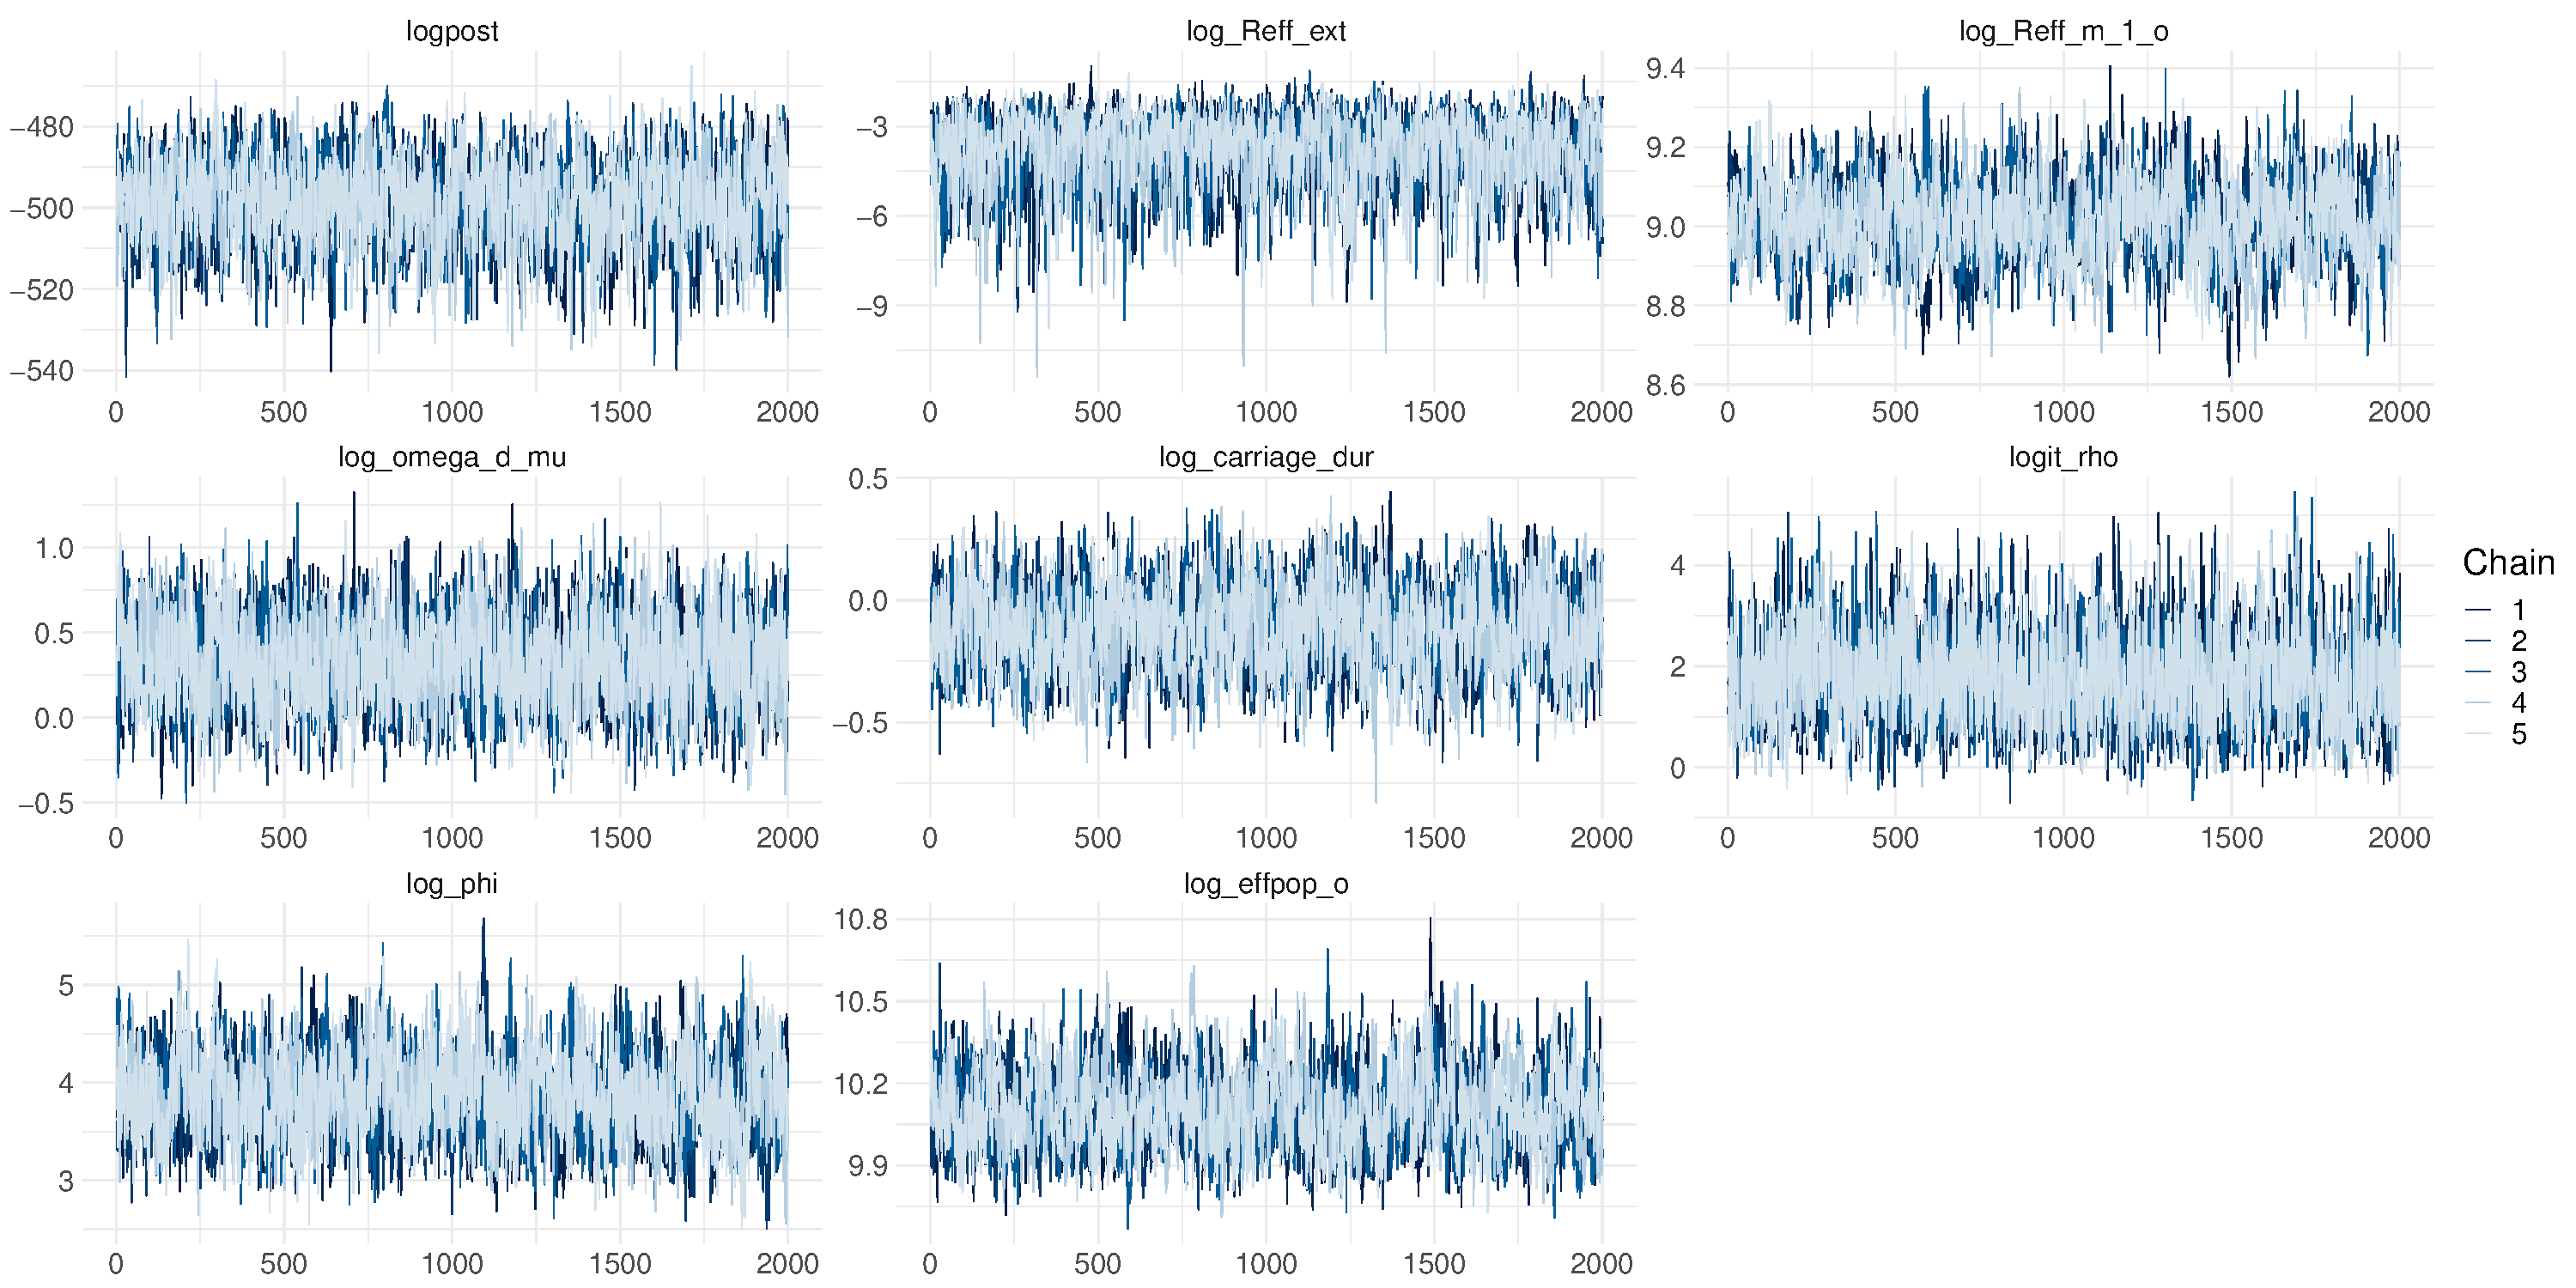
\includegraphics[width=\linewidth]{figures/sln_tight_traces}
	\caption{Posterior traceplots for the SEIR model fit to data from the Ebola outbreak in Sierra Leone.}
	\label{fig:sierraleonetraces}
\end{sidewaysfigure}

\begin{figure}[htbp]
	\centering
	\includegraphics[width=\linewidth]{figures/sln_tight_pairs}
	\caption{Scatterplots of parameters for the SEIR model fit to data from the Ebola outbreak in Sierra Leone.}
	\label{fig:sierraleonepairs}
\end{figure}

\begin{figure}[htbp]
	\begin{fullpage}
		\centering
		\includegraphics[width=0.8\linewidth]{figures/ebola_single_pacfs}
		\caption[Posterior predictive distributions of partial autocorrelations for the main country--specific SEIR models fit to data from the West Africa Ebola outbreak.]{Distributions of partial autocorrelations at lags 1, 2, and 3 for datasets generated under the full and partial posterior predictive distributions for the main country--specific SEIR models fit to data from the West Africa Ebola outbreak. Vertical red lines are the partial autocorrelations for the observed incidence data at the respective lags.}
		\label{fig:ebola_single_pacfs}
	\end{fullpage}
\end{figure}

\begin{sidewaysfigure}[htbp]
	\begin{fullpage}
		\centering
		\includegraphics[width=\linewidth]{figures/ebola_single_drawplots}
		\caption[Posterior distributions of LNA draws for the main country--specific SEIR models fit to data from the West Africa Ebola outbreak.]{Posterior distributions of the LNA draws for exposures, infections, and recoveries (blue boxplots) in the main country--specific SEIR models fit data from the Ebola outbreak in Guinea, Liberia, and Sierra Leone. The lower and upper whisker tips correspond to the $ 2.5^\mr{th} $ and $ 97.5^\mr{th} $ posterior quantiles, the lower and upper hinges to the $ 25^\mr{th} $ and $ 75^\mr{th} $ quantiles, and the middle hash mark to the posterior median. The solid red lines are the theoretical quantiles of the posterior predictive distribution (or equivalently, the prior distribution) of the LNA draws, drawn at the quantiles of a standard normal distribution corresponding to the boxplot quantiles. The green ticks are the estimated quantiles of the posterior predictive distributions of the LNA draws, accounting for boundary conditions on the state space of the latent process and obtained by simulating LNA paths from the posterior predictive distribution.  The posterior distributions of LNA draws are shaded according to the level of posterior shrinkage, computed as one minus the ratio of standard deviations of LNA draws in the posterior and prior.}
		\label{fig:ebola_single_drawplots}
	\end{fullpage}
\end{sidewaysfigure}

\newpage
\subsection{Details and Supplementary Results for Multi--Country Models}
\label{subsec:ebola_joint_supplement}

\subsubsection{Priors and MCMC details}
\label{subsubsec:ebola_joint_mcmc}

We fit stratified SEIR models to the Ebola incidence data from Guinea, Liberia, and Sierra Leone under two prior regimes given in Tables \ref{tab:ebola_priors_joint_tight} and \ref{tab:ebola_priors_joint_diffuse}. Cross--border transmission was incorporated into the rate of infection via virtual migration, as explained in Section \ref{subsec:ebola_synth}.  The model fitting procedure and priors were the same for both models, and were also the same for models fit via the LNA and ODE. We ran five chains for each model, initialized at random parameter values, for 200,000 iterations per chain. The model parameters, not including the initial compartment volumes, were jointly updated via MVNSS (see Section \ref{subsubsec:mvn_slice_sampling}). The empirical covariance for the MVNSS algorithm was adapted over the first 100,000 iterations using the gain factor sequence, $\gamma_n = 0.5(1 + 0.01n)^{-0.9}$. The contribution of isotropic Gaussian noise to the proposal was initialized at 0.001 and reduced throughout the adaptation phase according to the sequence $ \iota_n = 0.001(1 + 0.01n)^{-0.99} $. The covariance matrix was blocked by country with covariances for parameters belonging to different countries set to zero. Thus, country specific parameters were proposed jointly but were independent in the proposal. Migration parameters were blocked with parameters corresponding to the destination country. The initial compartment volumes were updated jointly with the LNA paths in an EllipSS step. The MCMC alternated between three ElliptSS and two MVNSS updates per MCMC iteration. The ElliptSS bracket width was reset after the first 5,000 MCMC iterations to $ \omega = 2\sqrt{2\log(10)}\sigma_{ElliptSS}$, where $ \sigma_{ElliptSS} $ was the standard deviation of the accepted angles over the initial iterations. The MCMC estimation scales for each country were parameterized as in Table \ref{tab:seir_params_est3} with the one addition being the log ratio of effective reproductive numbers, subtract one, for Guinea, $ \log\left ((R_{eff,G}^{(2)}-1)/(R_{eff,G}^{(1)}-1)\right ) $. Convergence was assessed visually by inspection of traceplots of posterior samples, and via potential scale reduction factors (PSRFs) \cite{brooks1998general} computed via the \texttt{coda} R package \cite{codapackage}. The models each took roughly three days to run. 

\begin{table}[htbp]
	\caption[Priors for initial compartment volumes for a stratified SEIR model fit to data from the Ebola outbreak in West Africa.]{Priors for the initial compartment volumes at the times when transmission commenced in each country for single country models fit to data from the Ebola outbreak in West Africa. The initial compartment volumes for each country are assigned independent truncated multivariate normal priors that respect the boundary conditions on the state space of compartment volumes for that country (explained in Section \ref{sec:lna_init_volumes}). If the population size for country A is $ N_A $, and the initial state probability is denoted $ \bp_{0,A} = \bX_{0,A}/N_A  = (S_{0,A}, E_{0,A}, I_{0,A}, R_{0,A})/N_A$, the prior is a truncated multivariate normal approximation of a multinomial distribution with mean $ N_A\bp_{0,A}$ and covariance $ N_A(\bP_{0,A} - \bp_{0,A}\bp_{0,A}^T) $.} 
	\label{tab:ebola_joint_initdist_priors}
	\centering
	\begin{tabular}{lc}
		\hline \textbf{Country} & \textbf{Prior mean initial volumes} ($ \bX_0 $) \\
		\hline
		Guinea & ($ 11.8\times10^6 -7.1$, 4, 3, 0.1) \\
		Liberia & ($ 4.4\times10^6 -5.1$, 3, 2, 0.1) \\
		Sierra Leone & ($ 7.1\times10^6 -5.1$, 3, 2, 0.1) \\
		\hline
	\end{tabular}
\end{table}

\begin{sidewaystable}[htbp]
	\begin{fullpage}
		\caption[Parameters and priors for a country--stratified SEIR model fit to the West Africa Ebola outbreak.]{Parameters for a country--stratified SEIR model fit to the West Africa Ebola outbreak, prior distributions, 95\% prior intervals, and references that informed the choice of priors. Subscripts, $ G,L,S, $ indicate specific countries, or generic countries $ A,B $ if a prior is shared. Effective reproduction numbers are defined with respect to the effective population size as $ R_{eff} = \beta N_{eff} /\mu $.}
		\label{tab:ebola_priors_joint_tight}
		\scriptsize
		\centering
		\begin{tabular}{lllrr}
			\hline
			\textbf{Parameter} &  \textbf{Interpretation} & \textbf{Prior} & \textbf{Median (95\% Interval)} & \textbf{References} \\ \hline
			$ R_{eff,G}^{(2)} / R_{eff,G}^{(1)} $ & Ratio of effective reproduction \#s &  LogNormal(0, 0.5$ ^2 $) & $ R_{eff,G}^{(2)} / R_{eff,G}^{(1)} = $ 1.00 (0.38, 2.66) & \cite{chowell2014transmission,chretien2015mathematical,coltart2017ebola,king2015avoidable} \\
			$ R_{eff,G}^{(2)}(t)-1 $ & Effective reproduction \# - 1, $ t\geq33 $ & LogNormal(log(0.5), $ 0.75^2 $) & $ \implies R_{eff,G}^{(2)} = 1.50 (1.11, 3.17)$ &  \cite{chowell2014transmission,chretien2015mathematical,coltart2017ebola,king2015avoidable} \\
			$ R_{eff,L} -1 $ & Effective reproduction \#-1 &  LogNormal(log(0.5), $ 0.75^2 $) & $ \implies R_{eff,L} = 1.50 (1.11, 3.17)$ &  \cite{chowell2014transmission,chretien2015mathematical,coltart2017ebola,king2015avoidable} \\
			$ R_{eff,S}-1 $ & Effective reproduction \#-1 & LogNormal(log(0.5), 0.75$ ^2 $) & $ \implies R_{eff,S} = 1.50 (1.11, 3.17)$ &  \cite{chowell2014transmission,chretien2015mathematical,coltart2017ebola,king2015avoidable}\\
			\makecell[l]{$ \alpha_{GS},\alpha_{GL}, \alpha_{LG},$\\
			$ \alpha_{LS},\alpha_{SG}, \alpha_{SL} $} & \makecell[l]{Infectious migration rate \\ from country A to B} & $ 1000\alpha_{AB} \sim$ Exponential(0.25) & \makecell[r]{\# migrations per 1000 infected \\ = 2.78 (0.10, 14.76)} & \cite{dudas2017virus}\\ 
			$ \omega_G/\omega_G $ & Rate from $ E_G\rightarrow I_G $ & LogNormal(0.0, 0.3$ ^2 $) & $ (1/\mu_G)\big/(1/\omega_G) $ = 1.00 (0.56, 1.80) & \cite{chowell2014transmission,velasquez2015time,glynn2017variability} \\
			$ \omega_L/\omega_L $ & Rate from $ E_L\rightarrow I_L $ & LogNormal(0.0, 0.3$ ^2 $) & $ (1/\mu_L)\big/(1/\omega_L) $ = 1.00 (0.56, 1.80) & \cite{chowell2014transmission,velasquez2015time,glynn2017variability} \\
			$ \omega_S/\omega_S $ & Rate from $ E_S\rightarrow I_S $ & LogNormal(0.0, 0.3$ ^2 $) & $ (1/\mu_S)\big/(1/\omega_S) $ = 1.00 (0.56, 1.80) & \cite{chowell2014transmission,velasquez2015time,glynn2017variability} \\
			$ 1/\mu_G $ & Rate from $ E_G\rightarrow I_G $ &  LogNormal(0.3, 0.2$ ^2 $) & $ 7/\mu_G = $ 9.45 (6.38, 13.98) & \cite{chowell2014transmission,velasquez2015time,glynn2017variability} \\
			$ 1/\mu_L $ & Rate from $ E_L\rightarrow I_L $ &  LogNormal(0.3, 0.2$ ^2 $) & $ 7/\mu_L = $ 9.45 (6.38, 13.98) & \cite{chowell2014transmission,velasquez2015time,glynn2017variability} \\
			$ 1/\mu_S $ & Rate from $ E_S\rightarrow I_S $ &  LogNormal(0.3, 0.2$ ^2 $) & $ 7/\mu_S = $ 9.45 (6.38, 13.98) & \cite{chowell2014transmission,velasquez2015time,glynn2017variability} \\
			$ N_{eff,G} $ & Effective population size & $\mr{Unif}(\sum_{\ell=1}^{L}Y_\ell^G, N_G/4) $& $ N_{eff,G} \in (3627,\ 2.95\times10^6) $ & Scale of counts \\
			$ N_{eff,L} $ & Effective population size & $\mr{Unif}(\sum_{\ell=1}^{L}Y_\ell^L, N_L/4) $& $ N_{eff,L} \in (4994,\ 1.1\times10^6) $ & Scale of counts \\
			$ N_{eff,S} $ & Effective population size & $\mr{Unif}(\sum_{\ell=1}^{L}Y_\ell^S, N_S/4) $& $ N_{eff,S} \in (11317,\ 1.775\times10^6) $ & Scale of counts \\
			$ \rho_G $ &  Mean case detection prob. & LogitNormal(0, 1.4$ ^2 $) & $ \implies \rho_G = 0.5, (0.06, 0.94)$ & Very high and very low $ \rho $ unlikely. \\
			$ \rho_L $ &  Mean case detection prob. & LogitNormal(0, 1.4$ ^2 $) & $ \implies \rho_L = 0.5, (0.06, 0.94)$ & Very high and very low $ \rho $ unlikely. \\
			$ \rho_S $ & Mean case detection prob. & LogitNormal(0, 1.4$ ^2 $) & $ \implies \rho_S = 0.5, (0.06, 0.94)$ & Very high and very low $ \rho $ unlikely. \\
			$ \phi_G,\ \phi_L, \phi_S $ &  Neg.Binomial overdispersion & LogNormal(0, 5$ ^2 $) & $ \implies \ = 1, (5.5\times 10^-5, 1.8\times10^4)$ & Diffuse. \\
			\hline
		\end{tabular}
	\end{fullpage}
\end{sidewaystable}

\begin{sidewaystable}[htbp]
	\begin{fullpage}
		\caption[Loose priors used in a sensitivity analysis for a stratified SEIR model for Ebola in West Africa.]{Priors for a sensitivity analysis for the country--stratified SEIR model fit to the West Africa Ebola outbreak. Priors were less informative priors for the effective reproductive numbers, cross--border transmission, and infectious period duration vis--a--vis the main model. Subscripts, $ G,L,S, $ indicate specific countries, or generic countries $ A,B $ if a prior is shared. Effective reproduction numbers are defined with respect to the effective population size as $ R_{eff} = \beta N_{eff} /\mu $.}
		\label{tab:ebola_priors_joint_diffuse}
		\scriptsize
		\centering
		\begin{tabular}{lllrr}
			\hline
			\textbf{Parameter} &  \textbf{Interpretation} & \textbf{Prior} & \textbf{Median (95\% Interval)} & \textbf{References} \\ \hline
			$ R_{eff,G}^{(2)} / R_{eff,G}^{(1)} $ & Ratio of effective reproduction \#s &  LogNormal(0, 0.5$ ^2 $) & $ R_{eff,G}^{(2)} / R_{eff,G}^{(1)} = $ 1.00 (0.38, 2.66) & \cite{chowell2014transmission,chretien2015mathematical,coltart2017ebola,king2015avoidable} \\
			$ R_{eff,G}^{(2)}(t)-1 $ & Effective reproduction \# - 1, $ t\geq33 $ & LogNormal(log(0.5), $ 1.5^2 $) & $ \implies R_{eff,G}^{(2)} = 1.50 (1.02, 10.46)$ &  \cite{chowell2014transmission,chretien2015mathematical,coltart2017ebola,king2015avoidable} \\
			$ R_{eff,L} -1 $ & Effective reproduction \#-1 &  LogNormal(log(0.5), $ 1.5^2 $) & $ \implies R_{eff,L} = 1.50 (1.02, 10.46)$ &  \cite{chowell2014transmission,chretien2015mathematical,coltart2017ebola,king2015avoidable} \\
			$ R_{eff,S}-1 $ & Effective reproduction \#-1 & LogNormal(log(0.5), 1.5$ ^2 $) & $ \implies R_{eff,S} = 1.50 (1.02, 10.46)$ &  \cite{chowell2014transmission,chretien2015mathematical,coltart2017ebola,king2015avoidable}\\
			\makecell[l]{$ \alpha_{GS},\alpha_{GL}, \alpha_{LG},$\\
				$ \alpha_{LS},\alpha_{SG}, \alpha_{SL} $} & \makecell[l]{Infectious migration rate \\ from country A to B} & $ 1000\alpha_{AB} \sim$ Exponential(0.125) & \makecell[r]{\# migrations per 1000 infected \\ = 5.55 (0.20, 29.51)} & \cite{dudas2017virus}\\ 
			$ \omega_G/\omega_G $ & Rate from $ E_G\rightarrow I_G $ & LogNormal(0.0, 0.3$ ^2 $) & $ (1/\mu_G)\big/(1/\omega_G) $ = 1.00 (0.56, 1.80) & \cite{chowell2014transmission,velasquez2015time,glynn2017variability} \\
			$ \omega_L/\omega_L $ & Rate from $ E_L\rightarrow I_L $ & LogNormal(0.0, 0.3$ ^2 $) & $ (1/\mu_L)\big/(1/\omega_L) $ = 1.00 (0.56, 1.80) & \cite{chowell2014transmission,velasquez2015time,glynn2017variability} \\
			$ \omega_S/\omega_S $ & Rate from $ E_S\rightarrow I_S $ & LogNormal(0.0, 0.3$ ^2 $) & $ (1/\mu_S)\big/(1/\omega_S) $ = 1.00 (0.56, 1.80) & \cite{chowell2014transmission,velasquez2015time,glynn2017variability} \\
			$ 1/\mu_G $ & Rate from $ E_G\rightarrow I_G $ &  LogNormal(0.3, 0.35$ ^2 $) & $ 7/\mu_G = $ 9.45 (4.76, 18.76) & \cite{chowell2014transmission,velasquez2015time,glynn2017variability} \\
			$ 1/\mu_L $ & Rate from $ E_L\rightarrow I_L $ &  LogNormal(0.3, 0.35$ ^2 $) & $ 7/\mu_L = $ 9.45 (4.76, 18.76) & \cite{chowell2014transmission,velasquez2015time,glynn2017variability} \\
			$ 1/\mu_S $ & Rate from $ E_S\rightarrow I_S $ &  LogNormal(0.3, 0.35$ ^2 $) & $ 7/\mu_S = $ 9.45 (4.76, 18.76) & \cite{chowell2014transmission,velasquez2015time,glynn2017variability} \\
			$ N_{eff,G} $ & Effective population size & $\mr{Unif}(\sum_{\ell=1}^{L}Y_\ell^G, N_G/4) $& $ N_{eff,G} \in (3627,\ 2.95\times10^6) $ & Scale of counts \\
			$ N_{eff,L} $ & Effective population size & $\mr{Unif}(\sum_{\ell=1}^{L}Y_\ell^L, N_L/4) $& $ N_{eff,L} \in (4994,\ 1.1\times10^6) $ & Scale of counts \\
			$ N_{eff,S} $ & Effective population size & $\mr{Unif}(\sum_{\ell=1}^{L}Y_\ell^S, N_S/4) $& $ N_{eff,S} \in (11317,\ 1.775\times10^6) $ & Scale of counts \\
			$ \rho_G $ &  Mean case detection prob. & LogitNormal(0, 1.4$ ^2 $) & $ \implies \rho_G = 0.5, (0.06, 0.94)$ & Very high and very low $ \rho $ unlikely. \\
			$ \rho_L $ &  Mean case detection prob. & LogitNormal(0, 1.4$ ^2 $) & $ \implies \rho_L = 0.5, (0.06, 0.94)$ & Very high and very low $ \rho $ unlikely. \\
			$ \rho_S $ & Mean case detection prob. & LogitNormal(0, 1.4$ ^2 $) & $ \implies \rho_S = 0.5, (0.06, 0.94)$ & Very high and very low $ \rho $ unlikely. \\
			$ \phi_G,\ \phi_L, \phi_S $ &  Neg.Binomial overdispersion & LogNormal(0, 5$ ^2 $) & $ \implies \ = 1, (5.5\times 10^-5, 1.8\times10^4)$ & Diffuse. \\
			\hline
		\end{tabular}
	\end{fullpage}
\end{sidewaystable}

\subsubsection{Additional results}
\label{subsubsec:ebola_joint_supp_res}

\begin{table}[htbp]
	\caption[Posterior estimates of initial numbers of exposed, infected, and recovered individuals for a stratified SEIR model fit to Ebola outbreak data.]{Posterior estimates of initial numbers of exposed, infected, and recovered individuals for the main stratified approximate SEIR model with virtual migration of infecteds fit to Ebola data from the West Africa outbreak under tight priors. The effective number of susceptibles is equal to the effective population size, reported in Table \ref{tab:ebola_joint_ests}, minus the numbers of exposed, infected, and recovered individuals, but is not reported since the effective population size is not marginally identifiable.}
	\label{tab:ebola_joint_initdist_res}
	\centering
	\begin{tabular}{ll}
		\hline
		\textbf{Parameter} & \textbf{Estimate }\\ 
		\hline
		$ E_{0,G} $&  4.3 (1.1, 7.8) \\ 
		$ E_{0,L} $&  3.4 (0.59, 6.6) \\ 
		$ E_{0,S} $&  2.3 (0.23, 5.5) \\ 
		$ I_{0,G} $& 3.4 (0.59, 6.6) \\ 
		$ I_{0,L} $&  2.6 (0.47, 5.1) \\ 
		$ I_{0,S} $& 2.4 (0.37, 4.8) \\ 
		$ R_{0,G} $& 0.1 (0.07, 0.2) \\ 
		$ R_{0,L} $&  0.1 (0.07, 0.2) \\ 
		$ R_{0,S} $&  0.1 (0.06, 0.2) \\ 
		\hline
	\end{tabular}
\end{table}

\begin{table}[htbp]
	\caption[Posterior parameter estimates for stratified SEIR models fit Ebola outbreak data.]{Posterior medians (95\% Bayesian credible intervals) for parameters of the approximate (Figure \ref{fig:stratified_seir_approx_diag}) stratified SEIR models fit to Ebola outbreak data. Subscripts, $ G,L,S, $ indicate specific countries, or generic countries $ A,B $. Effective reproduction numbers are defined with respect to the effective population size as $ R_{eff} = \beta N_{eff} /\mu $. Parameter interpretations and priors are given in Tables \ref{tab:ebola_priors_joint_tight} and \ref{tab:ebola_priors_joint_diffuse}. The more informative of the two prior regimes was presented as the main model in Section \ref{subsubsec:ebola_joint_model}.}
	\label{tab:ebola_joint_ests}
	\centering\footnotesize
	\begin{tabular}{crr}
		\hline
		& \multicolumn{2}{c}{\textbf{Posterior median (95\% BCI)}}\\\cline{2-3}
		\textbf{Parameter} & \textit{Tight Priors} & \textit{Loose Priors} \\ 
		\hline
		$ R_{eff,G}^{(1)} $& 1.1 (1, 1.3) & 1.1 (1, 1.2) \\ 
		$ R_{eff,G}^{(2)} $& 1.2 (1.1, 1.4) & 1.1 (1, 1.3) \\ 
		$ R_{eff,L} $& 2.1 (1.6, 3.3) & 1.8 (1.3, 3.4) \\ 
		$ R_{eff,S} $& 1.3 (1.1, 1.4) & 1.1 (1, 1.3) \\ 
		$ 7/\omega_G $& 7.5 (3.9, 13.6) & 5.6 (2.6, 11.4) \\ 
		$ 7/\omega_L $& 9 (4.1, 19.9) & 7.2 (2.5, 19.3) \\ 
		$ 7/\omega_S $& 4.1 (2.4, 6.6) & 3 (1.5, 5.4) \\ 
		$ 7/\mu_G $& 8.4 (5.9, 11.8) & 6.4 (3.6, 10.8) \\ 
		$ 7/\mu_L $& 9 (6, 13.2) & 7.5 (3.4, 15.5) \\ 
		$ 7/\mu_S $& 6.1 (4.4, 8.2) & 3.9 (2.4, 6.2) \\ 
		$ 1000\alpha_{GL} $& 3.0 (0.1, 15.5) & 6.3 (0.3, 29.8) \\ 
		$ 1000\alpha_{GS} $& 2.6 (0.1, 13.5) & 4.4 (0.2, 23.5) \\ 
		$ 1000\alpha_{LG} $& 3.9 (0.5, 14.2) & 6.5 (1, 20.5) \\ 
		$ 1000\alpha_{LS} $& 1.4 (0.1, 7.2) & 3 (0.2, 13.3) \\ 
		$ 1000\alpha_{SG} $& 2.6 (0.1, 13.4) & 4.7 (0.3, 25) \\ 
		$ 1000\alpha_{SL} $& 3.0 (0.1, 16.7) & 6.8 (0.2, 37.8) \\ 
		$ \rho_GN_{eff,G} $& 9900 (6600, 15600) & 14600 (7800, 29100) \\ 
		$ \rho_{L}N_{eff,L} $& 5900 (4800, 7900) & 6400 (4800, 11100) \\ 
		$ \rho_SN_{eff,S} $& 26800 (20600, 38700) & 39400 (24800, 85800) \\ 
		$ \phi_G $& 5.7 (3.4, 10.6) & 6.3 (3.6, 12.9) \\ 
		$ \phi_L $& 8.8 (4.1, 19.3) & 10.2 (4.7, 27.2) \\ 
		$ \phi_S $& 48 (22, 118) & 56 (25, 140) \\ 
		\hline
	\end{tabular}
\end{table}

\begin{table}[htbp]
	\caption{Effective sample sizes and potential scale reduction factors for the main stratified SEIR model with virtual migration of infecteds fit to data from the West Africa Ebola outbreak under tight priors.}
	\centering\footnotesize
	\begin{tabular}{lrr}
		\hline
		\textbf{Parameter} & \textbf{ESS} & \textbf{PSRF} \\ 
		\hline
		$ \log(R_{eff,G}^{(2)}/R_{eff,G}^{(1)}) $& 647 & 1.00 \\ 
		$ \log(R_{eff,G}^{(2)}) $& 626 & 1.01 \\ 
		$ \log(R_{eff,L}) $& 347 & 1.02 \\ 
		$ \log(R_{eff,S}) $& 459 & 1.08 \\ 
		$ \log(\omega_G/\mu_G) $& 1161 & 1.01 \\ 
		$ \log(\omega_L/\mu_L) $& 409 & 1.02 \\ 
		$ \log(\omega_S/\mu_S) $& 1217 & 1.01 \\ 
		$ \log(1/\mu_G) $& 1141 & 1.01 \\ 
		$ \log(1/\mu_L) $& 743 & 1.00 \\ 
		$ \log(1/\mu_S) $& 874 & 1.00 \\ 
		$ \log(1000\alpha_{GL}) $& 1583 & 1.00 \\ 
		$ \log(1000\alpha_{GS}) $& 972 & 1.02 \\ 
		$ \log(1000\alpha_{LG}) $& 292 & 1.04 \\ 
		$ \log(1000\alpha_{LS}) $& 478 & 1.02 \\ 
		$ \log(1000\alpha_{SG}) $& 1238 & 1.00 \\ 
		$ \log(1000\alpha_{SL}) $& 1198 & 1.06 \\ 
		$ \log(\rho_GN_{eff,G}) $& 725 & 1.00 \\ 
		$ \log(\rho_LN_{eff,L}) $& 521 & 1.01 \\ 
		$ \log(\rho_SN_{eff,S}) $& 479 & 1.04 \\ 
		$ \logit(\rho_G) $& 631 & 1.01 \\ 
		$ \logit(\rho_L) $& 217 & 1.04 \\ 
		$ \logit(\rho_S) $& 1414 & 1.01 \\ 
		$ \log(\phi_G) $& 596 & 1.03 \\ 
		$ \log(\phi_L) $& 1098 & 1.01 \\ 
		$ \log(\phi_S) $& 489 & 1.00 \\ 
		\hline
	\end{tabular}
\end{table}

\begin{sidewaysfigure}[htbp]
	\begin{fullpage}
		\centering
		\includegraphics[width=\linewidth]{figures/ebola_joint_posts}
		\caption[Posterior distributions of parameters of the main stratified SEIR model fit to data from the West Africa Ebola outbreak.]{Posterior distributions of parameters of the main stratified SEIR model fit to data from the West Africa Ebola outbreak under tight priors. We show posterior medians (solid gray lines), 95\% Bayesian credible intervals (light gray areas under the posterior densities), prior densities (induced priors for the reporting rate and latent period durations) over the posterior ranges (dashed green curves). $ R_{eff} = \beta N_{eff}/\mu $ is the effective reproductive number, where $ \beta $ is the per--contact infection rate, $ N_{eff} $ is the effective population size, and $ \mu $ is the recovery rate. The latent and infectious period durations, $ 7/\omega $ and $ 7/\mu $, respectively, are given in days. The effective number of cross--border infectious contacts in country $ B $ per 1000 infected individuals in country $ A $ is $ 1000\alpha_{AB} $. The effective reporting rate is $ \rho N_{eff} $, and $ \phi $ is the negative binomial over--dispersion parameter. Subscripts indicate countries.}
		\label{fig:ebola_joint_posts}
	\end{fullpage}
\end{sidewaysfigure}

\begin{sidewaysfigure}[htbp]
	\centering
	\includegraphics[width=\linewidth]{figures/ebola_joint_traces}
	\caption{Posterior traceplots for a stratified SEIR model fit to a simulated Ebola outbreak.}
	\label{fig:ebolajointtraces}
\end{sidewaysfigure}

\begin{figure}[htbp]
	\centering
	\includegraphics[width=\linewidth]{figures/ebola_joint_pairs_guin}
	\caption{Scatterplots of Guinea--specific parameters in a stratified SEIR model fit to data from the West Africa Ebola outbreak.}
\end{figure}

\begin{figure}[htbp]
	\centering
	\includegraphics[width=\linewidth]{figures/ebola_joint_pairs_lib}
	\caption{Scatterplots of Liberia--specific parameters in a stratified SEIR model fit to data from the West Africa Ebola outbreak.}
\end{figure}

\begin{figure}[htbp]
	\centering
	\includegraphics[width=\linewidth]{figures/ebola_joint_pairs_sln}
	\caption{Scatterplots of Sierra Leone--specific parameters in a stratified SEIR model fit to data from the West Africa Ebola outbreak.}
\end{figure}

\begin{figure}[htbp]
	\begin{fullpage}
		\centering
		\includegraphics[width=0.8\linewidth]{figures/ebola_joint_pacfs}
		\caption[Posterior predictive distributions of partial autocorrelations for a stratified SEIR model fit to data from the West Africa Ebola outbreak.]{Distributions of partial autocorrelations at lags 1, 2, and 3 for datasets generated under the full and partial posterior predictive distributions for the main stratified SEIR model fit to data from the West Africa Ebola outbreak. Vertical red lines are the partial autocorrelations for the observed incidence data at the respective lags.}
		\label{fig:ebola_joint_pacfs}
	\end{fullpage}
\end{figure}

\begin{sidewaysfigure}[htbp]
	\begin{fullpage}
		\centering
		\includegraphics[width=\linewidth]{figures/ebola_joint_drawplots}
		\caption[Posterior distributions of LNA draws for the main stratified SEIR model fit to data from the West Africa Ebola outbreak.]{Posterior distributions of the LNA draws for exposures, infections, and recoveries (blue boxplots) in the main stratified SEIR model fit data from the Ebola outbreak in Guinea, Liberia, and Sierra Leone. The lower and upper whisker tips correspond to the $ 2.5^\mr{th} $ and $ 97.5^\mr{th} $ posterior quantiles, the lower and upper hinges to the $ 25^\mr{th} $ and $ 75^\mr{th} $ quantiles, and the middle hash mark to the posterior median. The solid red lines are the theoretical quantiles of the posterior predictive distribution (or equivalently, the prior distribution) of the LNA draws, drawn at the quantiles of a standard normal distribution corresponding to the boxplot quantiles. The green ticks are the estimated quantiles of the posterior predictive distributions of the LNA draws, accounting for boundary conditions on the state space of the latent process and obtained by simulating LNA paths from the posterior predictive distribution. The posterior distributions of LNA draws are shaded according to the level of posterior shrinkage, computed as one minus the ratio of standard deviations of LNA draws in the posterior and prior.}
		\label{fig:ebola_joint_drawplots}
	\end{fullpage}
\end{sidewaysfigure}

\newpage
\section{LNA Implementation Details and LNA Model Vignettes}
\label{sec:lna_implementation_vignettes} % LNA methods appendix 
\chapter{Appendix to Chapter 5}
\label{chap:appendix_ch5}

\section{Simulation Details for Results in Section \ref{subsec:tparam_motivation}}
\label{sec:tparam_motiv_details}

\subsection{Simulation setup}
\label{subsec:tparam_motiv_setup}

We simulated an outbreak with SIRS dynamics in a population of $ N= 100,000$ individuals, ten of whom were initially infected, spanning two wave of the outbreak over thirty weeks. The mean infectious period duration was one week, and the mean duration of immunity was four weeks. The basic reproduction numbers of the outbreak, and hence the per--contact infectivity rates, varied sinusoidally with additive noise, over the course of the outbreak:
\begin{equation}
\label{eqn:sinfoi_true_R0t}
R0(t) = \beta(t) N / \mu = 2 + 0.35(\sin(t / 3.5) + 0.1Z_t),
\end{equation} 
where $ Z_t \sim N(0,1)$. The per--contact infection rates were then obtained as $ \beta(t) = R0(t) \mu / N $ The observed incidence was a negative binomial sample of the true incidence with mean case detection rate $ \rho $ and overdispersion parameter $ \phi $: 
\begin{equation}
Y_\ell \sim \mr{Neg.Binom.}\left (\mu  = \rho(N_{SI}(t_\ell) - N_{SI}(t_{\ell-1})), \sigma^2 = \mu(1 + \mu /\phi) \right ).
\end{equation}

\begin{table}[htbp]
	\caption[Parameters and priors for models fit two SIRS models to data from a simulated outbreak with sinusoidal FOI.]{Parameters and priors used in fitting two SIRS models, one with constant FOI and another with time--varying FOI, to data from an outbreak with SIRS dynamics where the per--contact infection rate varied sinusoidally over time.}
	\label{tab:tparam_sim_priors}
	\scriptsize\centering
	\begin{tabular}{clllr}
		\hline
		\textbf{Parameter} & \textbf{Interpretation} & \textbf{Truth} & \textbf{Prior} & \textbf{Median (95\% Interval)} \\ \hline
		$ R0-1 $ & Basic reproduction \#-1 & Eqn. \ref{eqn:sinfoi_true_R0t} & LogNormal(0, 0.5) & $ \implies R0(t_0) = $ 2.00 (1.14, 8.10) \\ 
		$ 1/\mu $ & Mean infectious period & 1&  LogNormal(0.05, 0.5)& 1.05 (0.39, 2.80) \\
		$ \rho/(1-\rho)  $ & Odds of case detection  &0.25&  LogNormal(-0.847, 0.5) & $ \implies \rho =$ 0.3 (0.14, 0.53) \\
		$ 1/\sqrt{\phi} $ & Neg.Binom. overdispersion & 50 & Exponential(5)& $ \implies \phi = 52 (1.84, 39000) $.  \\
		\hline
	\end{tabular}
\end{table}

We fit two models, one where the force of infection was constant over the course of the outbreak and another where the rates of infectious contact were time varying, with log--differences in the basic reproduction numbers penalized using a first order Gaussian Markov random field (GMRF) shrinkage prior where the standard deviation of the log--differences is given by $ \sigma_{RW1} $ (analogous to the models in Section \ref{sec:flu_tparam_models}). We employed non--centered parameterizations for both the LNA and the GMRF. The models were fit under informative priors, summarized in Table \ref{tab:tparam_sim_priors}. We ran five MCMC chains per model for 100,000 iterations per chain, alternating between five elliptical slice sampling (EllipSS) updates and one multivariate normal slice sampling (MVNSS) updates per MCMC iteration. The estimation scale on which the MCMC explored the parameter space was given by $\lbrace \log(R0(t_0)), \log(1/mu), \logit(\rho), 1/\sqrt(\phi) \rbrace$. The MVNSS proposal covariance matrix was adapted throughout the first 50,000 iterations, samples from which were subsequently discarded, using the gain factor sequence: the gain factor sequence, $\gamma_n = 0.5(1 + 0.01n)^{-0.99}$. The contribution of isotropic Gaussian noise to the MVNSS proposal was initialized at 0.001 and reduced throughout the adaptation phase according to the sequence $ \iota_n = 0.001(1 + 0.01n)^{-0.99} $. Convergence was assessed visually by inspection of traceplots of posterior samples, and via potential scale reduction factors (PSRFs) \cite{brooks1998general} computed via the \texttt{coda} R package \cite{codapackage}.

\newpage
\subsection{Additional results}
\label{subsec:sinfoi_supp_res}

\begin{figure}[htbp]
	\centering
	\includegraphics[width=\linewidth]{figures/sinfoi_rw1_traces}
	\caption{Posterior traceplots for SIRS model parameters with time--varying force of infection.}
	\label{fig:sinfoirw1traces}
\end{figure}

\begin{figure}[htbp]
	\centering
	\includegraphics[width=\linewidth]{figures/sinfoi_rw1_pairs}
	\caption{Posterior histograms and pairwise hexplots for SIRS model parameters with time--varying force of infection.}
	\label{fig:sinfoirw1pairs}
\end{figure}

\begin{figure}[htbp]
	\centering
	\includegraphics[width=\linewidth]{figures/sinfoi_const_traces}
	\caption{Posterior traceplots for SIRS model parameters with time--homogeneous force of infection.}
	\label{fig:sinfoiconsttraces}
\end{figure}

\begin{figure}[htbp]
	\centering
	\includegraphics[width=\linewidth]{figures/sinfoi_const_pairs}
	\caption{Posterior histograms and pairwise hexplots for SIRS model parameters with time--homogeneous force of infection.}
	\label{fig:sinfoiconstpairs}
\end{figure}

\begin{figure}[htbp]
	\centering
	\includegraphics[width=\linewidth]{figures/sinfoi_lna_drawplots}
	\caption[Posterior distributions of LNA draws for SIRS models with time--varying and constant force of infection.]{Posterior distributions of the LNA draws for infection, recovery, and loss of immunity in SIRS models with time--varying and constant force of infection (blue boxplots). The lower and upper whisker tips correspond to the $ 2.5^\mr{th} $ and $ 97.5^\mr{th} $ posterior quantiles, the lower and upper hinges to the $ 25^\mr{th} $ and $ 75^\mr{th} $ quantiles, and the middle hash mark to the posterior median. The solid red lines are the theoretical quantiles of the posterior predictive distribution (or equivalently, the prior distribution) of the LNA draws, drawn at the quantiles of a standard normal distribution corresponding to the boxplot quantiles. The green ticks are the estimated quantiles of the posterior predictive distributions of the LNA draws, accounting for boundary conditions on the state space of the latent process and obtained by simulating LNA paths from the posterior predictive distribution. The posterior distributions of LNA draws are shaded according to the level of posterior shrinkage, computed as one minus the ratio of standard deviations of LNA draws in the posterior and prior.}
	\label{fig:sinfoidrawplots}
\end{figure}

\newpage
\section{Specification of Contact Rates}
\label{sec:flu_contact_rates}

Contact rates within and between age--strata were obtained from the Finnish arm of the POLYMOD survey \cite{mossong2008social,polymod}, and were accessed via the \texttt{socialmixr R} package \cite{funk2018socialmixr}. The survey was a population--based, prospective survey that recorded contact rates by sex, age, location, duration, and frequency. We queried the symmetric form of the estimated mean contact matrix aggregated age--strata in our analysis (0--19 years and 20+ years), which based on a sample of 1,006 individuals. A contact matrix is said to be symmetric if the total number of contacts between two groups is equal. In particular, if $ c_{ij} $ is the mean number of contacts an individual in group $ i $ has with members of group $ j $, and group $ i $ is of size $ N_i $, then symmetry requires that $ c_{ij}N_i = c_{ji}N_j $. Due to the vagaries of sampling variability, this relation does not always hold. The symmetric contact matrix is obtained by taking $ c_{ij}^{\prime} = (c_{ij}N_i + c_{ji}N_j) / 2N_i $. 

The estimated mean contact rates are
\[ \bC_{tot} = 
\kbordermatrix{
	 & 0-19 & 20+ \\
	 0-19 & 7.44 & 5.05 \\
	 20+ & 1.55 & 8.56
}. \]
Following \cite{meyer2017incorporating}, we row--normalize the matrix, thus removing differences in absolute contact rates. This is helpful in parameterizing and assigning sensible priors to other aspects of the model, such as basic reproduction numbers. The normalized contact rates are
\[ \bC = 
\kbordermatrix{
	& 0-19 & 20+ \\
	0-19 & 0.60 & 0.40 \\
	20+ & 0.15 & 0.85
}. \]

\newpage
\section{Mapping Standard Normal Draws to LNA Sample Paths with Forcings}
\label{sec:dolna_forcings}
\begin{algorithm}[htbp]
	\caption{Mapping standard normal draws onto LNA sample paths with forcings.}
	\label{alg:doLNA2}
	\begin{algorithmic}[1]
		\Procedure{doLNA2}{$ \bZ,\btheta,\mcI,\bxi $}
		\State \textbf{initialize: }$ \bX(t_0) \gets \bX_0,\ \bN(t_0) \gets \bs{0},\ \bNtil(t_0) \gets \bs{0},\ \bmu(t_0) \gets \bs{0},\ \bSigma(t_0) \gets \bs{0} $
		\For{$ \ell = 1,\dots,L $}
		\State $ \bmu(t_\ell),\ \bSigma(t_\ell) \gets $ solutions to (\ref{eqn:lna_ode_drift}) and (\ref{eqn:lna_ode_diffusion}) over $ (t_{\ell-1}, t_\ell] $
		\State $ \bNtil(t_\ell)\gets \bmu(t_\ell) + \bSigma(t_\ell)^{1/2}\bZ(t_\ell) $ \Comment{non--centered parameterization}
		\State $ \bN(t_\ell)\gets \bN(t_{\ell-1}) + \exp(\bNtil(t_\ell)) - \bs{1} $
		\State \textbf{restart initial conditions:} 
		  \vspace{-0.15in}\hspace{0.2in} \begin{align*}
			\bX(t_\ell) &\gets \bX(t_{\ell-1}) + \bA^T(\bN(t_\ell)-\bN(t_{\ell-1})) \\
			\bX(t_\ell^+) &\gets \bX(t_\ell) + \bxi(t_\ell)\\
			\bNtil(t_\ell) &\gets \bs{0},\ \bmu(t_\ell)\gets\bs{0},\ \bSigma(t_\ell)\gets\bs{0}
			\end{align*}\vspace{-0.35in}
		\EndFor
		\State \hspace{-0.25in}\Return \Comment{return incidence and/or prevalence sample paths}
		\State$\bN = \left \lbrace\bN(t_0),\bN(t_1),\dots,\bN(t_L)\right \rbrace,\ \bX = \left \lbrace \bX(t_0),\ \bX(t_1),\dots,\bX(t_\ell) \right \rbrace $
		\EndProcedure
	\end{algorithmic}
\end{algorithm}

\newpage
\section{Joint Sampling of LNA Paths and Gaussian Markov Random Fields}
\label{sec:lna_ess_gmrf}

Jointly sampling the LNA draws and the values of a GMRF, $ \bF $, in addition to possibly any other latent Gaussian parameters including the initial compartment volumes as in Section \ref{sec:lna_init_volumes}, requires trivially modifying Algorithm \ref{alg:elliptss_lna_initvols} to include the additional parameters. We implement the same computational strategy used throughout Chapters \ref{chap:lna_for_sems} and \ref{chap:lna_extensions} of using non--centered parameterizations for the parameters of interest and the LNA path. As we have noted, this has the advantage of breaking the autocorrelation that would otherwise lead to poor MCMC mixing when using a centered parameterization and alternating between updates to different parameters in the model. We will denote by $ \bZ = (\bZ^X,\ \bZ^{X_0},\ \bZ^F,\ \bZ^{\btheta_F}) $ the multivariate standard normal draws for the latent LNA process, the initial compartment volumes, the draws to be mapped to the GMRF, and $ \bZ^{\btheta_F} $ the draws that are mapped to the GMRF hyper--parameters that are to be updated along with the GMRF. Unless otherwise stated (and we never do so state), we will at the very least update the precision or standard deviation of the GMRF increments jointly with the field to avoid poor MCMC mixing. We will assume that non--centered parameterizations for the GMRF and the hyper--parameters are linear transformations and thus do not require Jacobian terms to be included in the ElliptSS acceptance probability. We will denote by $ \bm_0 $, $ \bm_\theta $, $ \bV_0 $, and $ \bV_\theta $ the means and covariance matrices of the initial volumes and hyper--parameters, and by $ \doGMRF $ the linear operator for mapping $ \bZ^F $ to a GMRF sample, i.e., the GMRF values are obtained by $ \doGMRF(\bZ^F; \btheta_F) $. 

\begin{algorithm}[htbp]
	\caption{Sampling LNA draws, initial volumes, GMRF values, and GMRF hyper--parameters via elliptical slice sampling.}
	\label{alg:elliptss_lna_gmrf}
	\begin{algorithmic}[1]
		\Procedure{\doElliptSS3}{$ \bZ = (\bZ^X_{cur}, \bZ^{X_0}_{cur},\bZ^{F},\bZ^{\btheta_F}),\btheta,\bY,\mcI,\omega = 2\pi $}
		\State Sample ellipse: $ \bZ_{prop} \sim N(\bs{0}, \mb{I})$
		\State Sample threshold: $ u|\bx \sim \mr{Unif}(0, L(\bY|\doLNA(\bZ_{cur},\btheta,\mcI))) $
		\State Position the bracket: \vspace{-0.15in}
		\begin{align*}
		\psi &\sim \mr{Unif}(0,\omega)\\
		L_\psi &\leftarrow -\psi;\ R_\psi \leftarrow L_\psi + \psi\\
		\phi &\sim \mr{Unif}(L_\psi,R_\psi)
		\end{align*}
		\State Compute the proposal: \vspace{-0.1in}\begin{align*}
		\bZ^\prime &\leftarrow \bZ_{cur}\cos(\phi) + \bZ_{prop}\sin(\phi) \\
		&\implies \bX_0^\prime = \bm_0 + \bV_0^{1/2}\bZ^{X_0^\prime}\\
		&\implies\btheta_F^\prime = \bm_\theta + \bV_\theta^{1/2}\bZ^{\theta_F^\prime} \\
		&\implies\bF^\prime = \doGMRF(\bZ^F;\btheta_F)
		\end{align*}
		\If{$ L(\bY|\doLNA(\bZ^{X\prime},\bX_0^\prime,\bF^\prime,\btheta_F^\prime,\btheta,\mcI)) > u $}{ accept $ \bZ^\prime $}
		\State\Return{ $ \bZ' $}
		\Else
		\State Shrink bracket and try a new angle:
		\State{\textbf{If:} $ \phi < 0 $}{ \textbf{then: }$ L_\phi \leftarrow\phi $ }{ \textbf{else: }$ R_\phi \leftarrow \phi $}
		\State $ \phi \sim \mr{Unif}(L_\phi, R_\phi) $
		\State \textbf{GoTo:} 5
		\EndIf
		\EndProcedure
	\end{algorithmic}
\end{algorithm}

\section{Modeling Pandemic A(H1N1) Influenza in Finland --- Additional Details and Supplementary Results}
\label{sec:flu_supplement}

\subsection{MCMC Details}
\label{subsec:flu_mcmc_details}
We fit age--vaccination stratified SIRS ODE models with time varying dynamics to pandemic A(H1N1) influenza incidence data. The vaccination adjusted reproduction numbers were modeled using either a GMRF or as piecewise homogeneous within three epochs. The models were fit using the same prior regimes, given in Table \ref{tab:flu_priors}. We ran five chains for each model, initialized at random parameter values, for 100,000 iterations per chain. Model parameters (excluding noncentered GMRF draws and hyperparameters, as described in Section \ref{subsec:flu_mcmc}) were jointly updated via MVNSS (see Section \ref{subsubsec:mvn_slice_sampling}). The empirical covariance for the MVNSS algorithm was adapted over the first 50,000 iterations using the gain factor sequence, $\gamma_n = 0.5(1 + 0.01n)^{-0.9}$. The contribution of isotropic Gaussian noise to the proposal was initialized at 0.001 and reduced throughout the adaptation phase according to the sequence $ \iota_n = 0.001(1 + 0.01n)^{-0.99} $. In the GMRF model, the non--centered GMRF draws were updated via ElliptSS along with their hyperparameters, hence MCMC alternated between one ElliptSS and one MVNSS update per MCMC iteration. The ElliptSS bracket width was reset after the first 5,000 MCMC iterations to $ \omega = 2\sqrt{2\log(10)}\sigma_{ElliptSS}$, where $ \sigma_{ElliptSS} $ was the standard deviation of the accepted angles over the initial iterations. The MCMC estimation scales for the non--GMRF parameters were parameterized as in Table \ref{tab:flu_params_est}, and the GMRF was parameterized using the NCP given in Section \ref{subsec:flu_gmrf}. Convergence was assessed visually by inspection of traceplots of posterior samples. The models took between roughly one hour to run.

\subsection{Prior Specification}
\label{subsec:flu_priors}

\subsubsection{Priors for effective population sizes}
\label{subsubsec:flu_effpop_priors}

\subsubsection{Priors for time--homogeneous parameters}
\label{subsubsec:flu_param_priors_homog}

\begin{sidewaystable}[htbp]
	\begin{fullpage}
		\caption[Parameters and priors for age--vaccination stratified SIRS ODE models fit to the A(H1N1)pdm09 influenza outbreak in Finland.]{Parameters and priors for age--vaccination stratified SIRS ODE models fit to the A(H1N1)pdm09 influenza outbreak in Finland, prior distributions used in the main analysis. Vaccination adjusted intrinsic reproduction numbers are defined as in equation \ref{eqn:R0t_vacc}.}
		\label{tab:flu_priors}
		\scriptsize
		\centering
		\begin{tabular}{lllrr}
			\hline
			\textbf{Parameter} &  \textbf{Interpretation} & \textbf{Prior} & \textbf{Median (95\% Interval)} & \textbf{References} \\ \hline
			\hline
		\end{tabular}
	\end{fullpage}
\end{sidewaystable}

\subsubsection{Priors for GMRFs}
\label{subsubsec:flu_gmrf_priors}

\begin{figure}
	\centering
	\includegraphics[width=\linewidth]{figures/flu_RW1_prior}
	\caption{Induced prior distribution of for vaccination adjusted basic reproduction numbers A(H1N1)pdm09 influenza in Finland.}
	\label{fig:flurw1prior}
\end{figure}


\subsection{Additional Results}
\label{subsec:flu_additional_results}

\subsubsection{Stratified SIRS model with time--varying dynamics}
\label{subsubsec:flu_additional_res_rw1}

\begin{sidewaysfigure}[htbp]
	\centering
	\includegraphics[width=\linewidth]{figures/flu_traces_rw_ode}
	\caption{Posterior traceplots for a stratified SIRS ODE model with time--varying dynamics fit to data from the A(H1N1) influenza pandemic in Finland.}
	\label{fig:flutracesrwode}
\end{sidewaysfigure}

\begin{sidewaysfigure}[htbp]
	\centering
	\includegraphics[width=\linewidth]{figures/flu_rw_pairs}
	\caption{Histograms and pairwise scatterplots of posterior samples for the parameters of a stratified SIRS ODE model with time varying dynamics that were sampled via MVNSS. The model was fit to data from the A(H1N1) influenza pandemic in Finland.}
	\label{fig:flurwpairs}
\end{sidewaysfigure}

\newpage

\subsubsection{Stratified SIRS model with piecewise--homogeneous dynamics}
\label{subsubsec:flu_additional_res_const}

\begin{sidewaystable}[htbp]
	\begin{fullpage}
		\caption[Parameters and priors for age--vaccination stratified SIRS ODE models fit to the A(H1N1)pdm09 influenza outbreak in Finland.]{Parameters and priors for age--vaccination stratified SIRS ODE models fit to the A(H1N1)pdm09 influenza outbreak in Finland, prior distributions used in the main analysis. Vaccination adjusted intrinsic reproduction numbers are defined as in equation \ref{eqn:R0t_vacc}.}
		\label{tab:flu_priors_const}
		\scriptsize
		\centering
		\begin{tabular}{lllrr}
			\hline
			\textbf{Parameter} &  \textbf{Interpretation} & \textbf{Prior} & \textbf{Median (95\% Interval)} & \textbf{References} \\ \hline
			\hline
		\end{tabular}
	\end{fullpage}
\end{sidewaystable}

\begin{sidewaysfigure}[htbp]
	\centering
	\includegraphics[width=\linewidth]{figures/flu_traces_const_ode}
	\caption{Posterior traceplots for a stratified SIRS ODE model with piecewise--homogeneous dynamics fit to data from the A(H1N1) influenza pandemic in Finland.}
	\label{fig:fluconstodetraces}
\end{sidewaysfigure}


\begin{sidewaysfigure}[htbp]
	\centering
	\includegraphics[width=\linewidth]{figures/flu_const_pairs}
	\caption{Histograms and pairwise scatterplots of posterior samples for the parameters of a stratified SIRS ODE model with piecewise homogeneous dynamics that were sampled via MVNSS. The model was fit to data from the A(H1N1) influenza pandemic in Finland.}
	\label{fig:fluconstpairs}
\end{sidewaysfigure}

\subsection{Sensitivity to Distribution of Initial Numbers of Susceptibles}
\label{subsec:flu_highsusc_sensitivity} % Flu analysis appendix

\end{document}
